\documentclass[12pt, a4paper, oneside]{extbook}

%\fontsize{14}{1.25}
\usepackage[T1]{fontenc}
\usepackage[utf8]{inputenc}
\usepackage[russian]{babel}

% margins
%\setlength{\textwidth}{360pt}
%\setlength{\oddsidemargin}{22pt}
%\setlength{\evensidemargin}{70pt}
%\setlength{\marginparwidth}{106pt}

% page margin
%\usepackage[top=2cm, bottom=2cm, left=2cm, right=2cm]{geometry}
\usepackage[left=2cm,right=2cm,top=2cm,bottom=2cm,bindingoffset=0cm]{geometry}

% AMS packages
\usepackage{amsmath}
\usepackage{amssymb}
\usepackage{amsfonts}
\usepackage{amsthm}

% floating option for figures
\usepackage{float}

\usepackage{xcolor}

\usepackage{bbm}

\usepackage{fancyhdr}
\pagestyle{fancy}
% modifying page layout using fancyhdr
\fancyhf{}
\renewcommand{\sectionmark}[1]{\markright{\thesection\ #1}}
\renewcommand{\subsectionmark}[1]{\markright{\thesubsection\ #1}}

\rhead{\fancyplain{}{\rightmark }}
\cfoot{\fancyplain{}{\thepage }}

\usepackage{array}
\usepackage{braket}

\makeatletter
\def\env@dmatrix{\hskip -\arraycolsep
  \let\@ifnextchar\new@ifnextchar
  \extrarowheight=2ex
  \array{*\c@MaxMatrixCols{>{\displaystyle}c}}}

\newenvironment{dmatrix}
  {\env@dmatrix}
  {\endarray\hskip-\arraycolsep}

\newenvironment{bdmatrix}
  {\left[\env@dmatrix}
  {\endmatrix\right]}
\makeatother

\newcommand{\mf}{\mathbf}

\newcommand{\lb}{\left(}
\newcommand{\rb}{\right)}
\newcommand{\lsq}{\left[}
\newcommand{\rsq}{\right]}
\newcommand{\lc}{\left\{}
\newcommand{\rc}{\right\}}

\newcommand{\bbI}{\mathbb{I}}
\newcommand{\bba}{\mathbbm{a}}
\newcommand{\bbA}{\mathbb{A}}
\newcommand{\bbB}{\mathbb{B}}
\newcommand{\bbG}{\mathbb{G}}
\newcommand{\bbM}{\mathbb{M}}
\newcommand{\bbV}{\mathbb{V}}
\newcommand{\bbW}{\mathbb{W}}
\newcommand{\EOmega}{\boldsymbol{\Omega}_{\rm \textbf{e}}}
\newcommand{\mfpe}{\mf{p_e}}
\newcommand{\mfpet}{\mf{p_e^+}}
\newcommand{\mfq}{\mf{q}}
\newcommand{\mfp}{\mf{p}}
\newcommand{\mfJ}{\mf{J}}

\DeclareMathAlphabet{\mymathbb}{U}{BOONDOX-ds}{m}{n}
\newcommand{\bbzero}{\mymathbb{0}}
\newcommand{\bbone}{\mymathbb{1}}

\def\hh{_{\rm H}}

\usepackage[toc]{appendix}

\usepackage{chngcntr}
\usepackage{etoolbox}
\AtBeginEnvironment{subappendices}{%
\chapter*{Appendix}
\addcontentsline{toc}{chapter}{Appendices}
\counterwithin{figure}{section}
\counterwithin{table}{section}
}

\usepackage{mathtools}

\DeclarePairedDelimiter\abs{\lvert}{\rvert}%
\DeclarePairedDelimiter\norm{\lVert}{\rVert}%

% Swap the definition of \abs* and \norm*, so that \abs
% and \norm resizes the size of the brackets, and the 
% starred version does not.
\makeatletter
\let\oldabs\abs
\def\abs{\@ifstar{\oldabs}{\oldabs*}}
%
\let\oldnorm\norm
\def\norm{\@ifstar{\oldnorm}{\oldnorm*}}
\makeatother

\newcommand{\bnp}[1]{b_n^{(#1)}}

% hyperlinks for eqref and cite
\usepackage{hyperref}

% indentation in the first paragraph of section or paragraph
\usepackage{indentfirst}

\newcommand{\boltz}{k_\text{b}}
\newcommand{\kb}{k_\text{b}}
\newcommand{\intty}{\int\limits_{-\infty}^\infty}
\newcommand{\mean}[1]{\langle #1 \rangle}
\newcommand{\bs}{\boldsymbol}
\newcommand{\mL}{\mathcal{L}}
\newcommand{\mH}{\mathcal{H}}
\newcommand{\mN}{\mathcal{N}}
\newcommand{\mHplane}{\mathcal{H}_\text{plane}}
\newcommand{\bbS}{\mathbb{S}}
\newcommand{\bxi}{\boldsymbol{\xi}}
\newcommand{\rfixed}{r_\text{fixed}}

\usepackage[raggedright]{titlesec}
\usepackage{fourier, erewhon}
\usepackage{microtype}
 \SetTracking[no ligatures={f}]{encoding=*}{100}
% changing fontsize of chapter titles
 \titleformat{\chapter}[display]
 {\bfseries\Large\lsstyle\SetTracking[no ligatures = {f}]{encoding = *}{50}\filleft}
 {\MakeUppercase{\chaptername}\enspace\thechapter}
 {2ex}
 {\titlerule[1pt]\vspace{2ex}\MakeUppercase}%
\titlespacing*{\chapter}{0pt}{-60pt}{10ex}

% changing fontsize of section titles
\titleformat{\section}
 {\normalfont\fontsize{16}{15}\bfseries}{\thesection}{1em}{}


\begin{document}

\tableofcontents

\chapter{Введение}
\iffalse
Homonuclear diatomic molecules, which includes several astrophysically and atmo-
spherically relevant species, have zero electric dipole moment due to their inversion
symmetry. This means that these molecules are in principle infrared inactive. How-
ever, gases of apolar molecules exhibit collision-induced absorption, as was first shown
experimentally for a gas of oxygen molecules.[10] This absorption originates from col-
lision complexes present in the gas. The collision complex can be considered to be a
short-lived species, which may have a lower symmetry than the individual molecules
and hence an electric dipole moment. Since these collision complexes are short-lived,
the resulting absorption spectra are typically broad in frequency.

Поглощение света описывается законом Бугера-Ламберта-Бера 
\begin{gather}
    I = I_0 \exp \lb - \alpha l \rb. 
\end{gather}
По закону Бера коэффицициент поглощения $\alpha$ связан линейно с плотностью поглощающего газа $n$
\begin{gather}
    \alpha = \sigma n,
\end{gather}
где через $\sigma$ обозначено сечение поглощения. Зависимость предполагает, что поглощение происходит индивидуальными молекулами. В общем случае, для описания этой зависимости может быть использовано вириальное разложение
\begin{gather}
    \alpha = \sigma n + \alpha_\text{binary} n^2 + \alpha_\text{ternary} n^3 + O(n^4), 
\end{gather}
в котором квадратичное слагаемое описывает столкновительно-индуцированное поглощение бинарными комплексами, кубическое слагаемое -- тройными комплексами, и т.д. Стоит отметить, что сечение поглощения мономера $\sigma$ зависит от давления (проявляется это, например, в сдвигах и уширениях линий), поэтому при каждой фиксированной частоте поглощение мономера не является линейным по плотности $n$, однако интегральная интенсивность линейна по плотности. \par
Таким образом, для моделирования суммарного профиля поглощения необходимо знать сечение поглощения $\sigma$, коэффициент бинарного поглощения $\alpha_\text{binary}$, и т.д., и как эти эти величины зависят от атмосферных характеристик, таких как температура. Данная работа посвящена расчет коэффициентов бинарного поглощения $\alpha_\text{binary}$ для различных систем, имеющих практическую значимость в атмосферных приложениях. \par
Спектры плотных газов и газовых смесей существенно отличаются от спектров, зарегистрированных при низких плотностях. По мере увеличения плотности, наблюдается линейное увеличение интенсивностей разрешенных колебательно-вращательных и электронных полос. При промежуточных значениях плотности могут возникнуть новые полосы поглощения, которые не наблюдались при более низких плотностях, причем интенсивность этих полос (по крайней мере в первом приближении) может быть описана квадратичным или кубическим законом. За появление этих полос отвественны ван дер Ваальсовы комплексы двух или большего количества молекул. Подобные полосы поглощения найдены во многих молекулярных газах, даже молекулы которых не обладают постоянным дипольным моментом.  

Состояния ван дер Ваальсовых комплексов классифицируют на связанные, полная колебательно-вращательная энергия меньше энергии диссоциации, и свободные. 

Впервые квадратичную зависимость коэффициента поглощения от плотности наблюдал Йенсен (Janssen) в 1885 году на полосах поглощениях кислорода \cite{janssen1885}.
\fi


\chapter{Теоретическое введение}
\section{Взаимодействие электромагнитного излучения с молекулярными системами}
Рассмотрим систему из $N$ взаимодействующих частиц (молекул) в квантовом состоянии $\ket{j}$. Обозначим гамильтониан системы через $\hat{H}_0$. Пусть система подвергается воздействию электрического поля частоты $\omega$, которое индуцирует переходы в другие состояния системы $\ket{k}$ при условии, что частота поля близка к частотам Бора системы
%
\begin{gather}
    \omega_{jk} = (E_j - E_k) / \hbar.
\end{gather}

Будем считать, что длина волны рассматриваемого поля $\lambda$ много больше размеров молекул в системе, поэтому в локальной окрестности молекул поле можно считать однородным в пространстве.  Электрическая составляющая электромагнитной волны может быть записана в виде суммы
%
\begin{gather}
    \mf{E}(t) = E_0 \boldsymbol{\varepsilon} \cos \omega t = \frac{E_0 \boldsymbol{\varepsilon}}{2} \lb e^{i \omega t} + e^{- \omega t} \rb,
\end{gather}
%
где $E_0$ -- амплитуда волны, а $\boldsymbol{\varepsilon}$ -- единичный вектор, направленный вдоль направления распространения волны. Энергия взаимодействия молекулярной системы с электрическим полем в дипольном приближении равна
%
\begin{gather}
    W(t) = - (\boldsymbol{\mu} \cdot \mf{E}) = - \frac{E_0}{2} \lb \boldsymbol{\mu} \cdot \boldsymbol{\varepsilon} \rb \lsq e^{i \omega t} + e^{-i \omega t} \rsq, \label{part1-dipole-approximation} 
\end{gather}
%
где через $\boldsymbol{\mu}$ обозначен полный дипольный момент системы. Взаимодействие молекулярных систем с электромагнитным полем часто рассматривают в этом приближении, считая поле классическим объектом. Уравнение \eqref{part1-dipole-approximation} подразумевает, что взаимодействие между полем и молекулярной системой исчезает, когда напряженность поля $\mf{E}$ равна 0. Однако это не так, иначе бы не наблюдалось явления спонтанного излучения. Связь между электромагнитным полем и системой должна быть двухсторонней, наличие поля может вызывать изменения в состоянии системы, но и наличие системы может изменять состояние поля. \par  
Взаимодействие молекулярных систем с электрическим полем традиционно рассматривается в рамках временной теории возмущений \cite{cohentanuji, greiner}. Согласно приложению А, вероятность индуцированного возмущением $W(t)$ перехода между состояниями невозмущенной системы $\ket{j} \rightarrow \ket{k}$ в первом порядке временной теории возмущения равна
%
\begin{gather}
    \mathcal{P}_{jk}(t) = \frac{1}{\hbar^2} \abs{ \int\limits_0^t W_{jk}(t^\prime) e^{i \omega_{jk} t^\prime} dt^\prime }^2,
\end{gather}
%
где через $W_{jk}(t)$ обозначен матричный элемент возмущения на состояниях невозмущенной системы, равный в данном случае
%
\begin{gather}
    W_{jk} = -\frac{E_0}{2} \bra{j} \boldsymbol{\mu} \cdot \boldsymbol{\varepsilon} \ket{k} \lsq e^{i \omega t} + e^{-i \omega t} \rsq.
\end{gather}

Коэффициенты разложения первого порядка $b_n^{(1)}(t)$ возмущенной волновой функции $\ket{\psi(t)}$ в базисе собственных функций невозмущенного гамильтониана равны (см. соотношение \eqref{app-expansion})
\begin{gather}
    b_{n}^{(1)}(t; \omega) = -\frac{E_0}{2 \hbar} \bra{j} \boldsymbol{\mu} \cdot \boldsymbol{\varepsilon} \ket{k} \lsq \frac{e^{i (\omega_{jk} + \omega) t} - 1}{\omega_{jk} + \omega} + \frac{e^{i (\omega_{jk} - \omega) t} - 1}{\omega_{jk} - \omega} \rsq. \label{part1-bn-expression}
\end{gather}
%
Квадрат модуля коэффициента $b_{n}^{(1)}$ определяет вероятность перехода в $n$-ое стационарное состояние невозмущенного гамильтониана. Возводя в квадрат выражение \eqref{part1-bn-expression}, после алгебраических преобразований приходим к
%
\begin{gather}
    \hspace*{-0.5cm}
    \abs{b_{n}^{(1)}(t)}^2 = \frac{E_0}{\hbar^2} \lsq \frac{\sin^2 \lb \frac{1}{2} \lb \omega_{jk} + \omega \rb t \rb}{\lb \omega_{jk} + \omega \rb^2} + \frac{\sin^2 \lb \frac{1}{2} \lb \omega_{jk} - \omega \rb t \rb}{\lb \omega_{jk} - \omega \rb^2} + \frac{ 8 \cos \lb \omega t \rb \sin \lb \frac{1}{2} \lb \omega_{jk} + \omega \rb t \rb \sin \lb \frac{1}{2} \lb \omega_{jk} - \omega \rb t \rb}{\lb \omega_{jk} + \omega \rb \lb \omega_{jk} - \omega \rb} \rsq. \label{part1-bn-expression2}
\end{gather}
 
В данном контексте нас интересуют не вероятности переходов, а скорости переходов $\Gamma_{jk}$ (иными словами, вероятности $P_{jk}$, отнесенные к единице времени) при больших значениях $t$
%
\begin{gather}
    \Gamma_{jk} = \lim_{t \rightarrow \infty} \frac{P_{jk}}{t}.
\end{gather}
%
При предельном переходе в \eqref{part1-bn-expression2} первые два слагаемые преобразуются к дельта-функционалам, в то время как последнее слагаемое оказывается нулевым \cite{baym-quantum-mechanics}. Итак, выражение для скорости переходов оказывается следующим \cite{mcquarrie-statistical-mechanics}  
%
\begin{gather}
    \Gamma_{jk} = \frac{\pi E_0^2}{2 \hbar^2} \abs{ \bra{j} \boldsymbol{\mu} \cdot \boldsymbol{\varepsilon} \ket{k} }^2 \Big[ \delta \lb \omega_{jk} - \omega \rb + \delta \lb \omega_{jk} + \omega \rb \Big]. \label{part1-transition-rate} 
\end{gather}

Выражение \eqref{part1-transition-rate} определяет скорость переходов между конкретными состояниями невозмущенной системы $\ket{j}$ и $\ket{k}$. Скорость поглощения энергии в ходе переходов между этими состояниями равна $\hbar \omega_{jk} \Gamma_{jk}$, т.к. в ходе одно акта поглощения, система поглощает энергию, равную $\hbar \omega_{jk}$. Скорость поглощения энергии в ходе переходов с заданного уровня $\ket{j}$ может быть получена при суммировании по всем состояниям $\ket{k}$, которые доступны системе для перехода. Наконец, суммарная скорость поглощения излучения системой $-\dot{E}_\text{rad}$ получается в результате суммирования по всем возможным начальным состояниям $\ket{j}$ с соответствующими заселенностями $\rho_j$
\begin{gather}
    -\dot{E}_\text{rad} = \sum_j \sum_k \rho_j \hbar \omega_{jk} \Gamma_{jk} = \frac{\pi E_0^2}{2 \hbar} \sum_{j, k} \omega_{jk} \rho_j \abs{ \bra{j} \boldsymbol{\mu} \cdot \boldsymbol{\varepsilon} \ket{k} }^2 \Big[ \delta \lb \omega_{jk} - \omega \rb + \delta \lb \omega_{jk} + \omega \rb \Big]. \label{part1-energy-absorption-rate}
\end{gather}

Для получения более симметричной формы уравнения \eqref{part1-energy-absorption-rate} осуществим алгебраические преобразования. Рассмотрим отдельно вторую сумму, получающуюся при раскрытии скобок в уравнении \eqref{part1-energy-absorption-rate}. Поменяем местами индексы $j \leftrightarrow k$, что обосновывается тем, что оба индекса пробегают по всем квантовым состояниям системы,
\begin{gather}
    \frac{\pi E_0^2}{2 \hbar} \sum_{j, k} \omega_{jk} \rho_j \abs{ \bra{j} \boldsymbol{\mu} \cdot \boldsymbol{\varepsilon} \ket{k} }^2 \delta \lb \omega_{jk} + \omega \rb = -\frac{\pi E_0^2}{2 \hbar} \sum_{j, k} \omega_{jk} \rho_j \abs{ \bra{j} \boldsymbol{\mu} \cdot \boldsymbol{\varepsilon} \ket{k} }^2 \delta \lb \omega_{jk} - \omega \rb. \label{part1-index-change}
\end{gather}

Подстановка \eqref{part1-index-change} в \eqref{part1-energy-absorption-rate} приводит к выражению, в котором индексы $j$ и $k$ входят симметричным образом 
%
\begin{gather}
    -\dot{E}_\text{rad} = \frac{\pi E_0^2}{2 \hbar} \sum_{j, k} \omega_{j k} \lb \rho_j - \rho_k \rb \abs{ \bra{j} \boldsymbol{\mu} \cdot \boldsymbol{\varepsilon} \ket{k} }^2 \delta \lb \omega_{jk} - \omega \rb.
\end{gather}

Предположим, что возмущение достаточно слабо и действует на протяжении малого промежутка времени, таким образом, что в любой момент система находится в состоянии теплового равновесия при температуре $T$. Используя это предположение, выразим заселенность $k$-ого состояния через заселенность $j$-го состояния (понятно, что можно воспользоваться и обратной связью, т.к. мы специально привели формулу к симметричному виду относительно замены индексов)
%
\begin{gather}
    \rho_k = \rho_j \exp \lb - \beta \hbar \omega_{jk} \rb,
\end{gather}
%
где $\beta = \boltz T$ и $\boltz$ -- постоянная Больцмана. Кроме того, вследствие того, что внутри суммы находятся дельта-функционалы, центрированные на $\omega_{jk}$ , функции от $\omega$, вычисленные при частоте $\omega_{jk}$, могут быть вынесены из под знака суммы: 
\begin{align}
    -\dot{E}_\text{rad} &= \frac{\pi E_0^2}{2 \hbar} \sum_{j, k} \omega_{jk} \rho_j \lb 1 - \exp \lb - \beta \hbar \omega_{jk} \rb \rb \abs{ \bra{j} \boldsymbol{\mu} \cdot \boldsymbol{\varepsilon} \ket{k} }^2 \delta \lb \omega_{jk} - \omega \rb = \\
    &= \frac{\pi E_0^2}{2 \hbar} \omega \lb 1 - \exp \lb - \beta \hbar \omega \rb \rb \sum_{j, k} \rho_j \abs{ \bra{j} \boldsymbol{\mu} \cdot \boldsymbol{\varepsilon} \ket{k} }^2 \delta \lb \omega_{jk} - \omega \rb. 
\end{align}

Суммарный поток энергии $I$, переносимой электромагнитной волной через среду с показателем преломления $n$, равен усредненному по времени модулю вектора Пойнтинга $\langle S \rangle$ и равен \cite{landau-volume2}
\begin{gather}
    I = \langle S \rangle = \frac{c}{8 \pi} n E_0^2,
\end{gather}
%
где $c$ -- скорость света в вакууме. Показатель поглощения среды $\alpha(\omega)$ определяют как отношение энергии, поглощаемой средой в единицу времени при частоте $\omega$, к энергии, переносимой электромагнитной волной в единицу времени \cite{mcquarrie-statistical-mechanics}
\begin{gather}
    \alpha(\omega) = \frac{-\dot{E}_\text{rad}}{I} = \frac{4 \pi^2}{\hbar c n} \omega \lb 1 - e^{- \beta \hbar \omega} \rb \sum_{j, k} \rho_j \abs{ \bra{j} \boldsymbol{\mu} \cdot \boldsymbol{\varepsilon} \ket{k}}^2 \delta \lb \omega_{jk} - \omega \rb. \label{part1-absorption-coefficient-definition}
\end{gather}

На основании выражения \eqref{part1-absorption-coefficient-definition} определяют \textit{спектральную функцию} $J(\omega)$ \cite{gordon1968}
\begin{gather}
    J(\omega) = \frac{3 \hbar c n \alpha(\omega)}{4 \pi^2 V \omega \lb 1 - e^{-\beta \hbar \omega} \rb} = 3 \sum_{j, k} \rho_j \abs{ \bra{j} \boldsymbol{\mu} \cdot \boldsymbol{\varepsilon} \ket{k} }^2 \delta \lb \omega_{jk} - \omega \rb. \label{part1-spectral-function-definition}
\end{gather}

Отметим, что обычно спектральную функцию определяют таким образом, чтобы ее интеграл по частотному диапазону был равен единице. Здесь принято несколько иное определение, эта функция не нормирована. \par
Альтернативную форму выражения \eqref{part1-spectral-function-definition} получают осуществляя смену Шредингеровского представления квантовой механики на представление Гейзенберга. Состояния в представлении Гейзенберга не зависят от времени -- временная эволюция заложена в операторах. Эволюция оператора $\hat{A}(t)$ описывается оперетором эволюции $U(t)$
\begin{gather}
    \hat{A}(t) = U^{+}(t) A(0) U(t) = e^{\frac{i}{\hbar} H t} \hat{A}(0) e^{-\frac{i}{\hbar} H t}. 
\end{gather}

Удобно перейти в выражении \eqref{part1-spectral-function-definition} к представлению Гейзенберга, представив дельта-функционал как Фурье-образ мнимой экспоненты
\begin{gather}
    \delta (\omega) = \frac{1}{2\pi} \int\limits_{-\infty}^\infty e^{i \omega t} dt,
\end{gather}
получаем
\begin{gather}
    J(\omega) = \frac{3}{2\pi} \sum_{j,k} \rho_j \bra{j} \boldsymbol{\mu} \cdot \varepsilon \ket{k} \bra{k} \boldsymbol{\mu} \cdot \boldsymbol{\varepsilon} \ket{j} \int\limits_{-\infty}^\infty \exp \lsq \lb \frac{E_j - E_k}{\hbar} - \omega \rb t \rsq dt. \label{part1-spectral-function-2}
\end{gather}

Т.к. состояния $\ket{k}$ и $\ket{j}$ являются собственными состояниями гамильтониана $\hat{H}_0$, то
\begin{gather}
    \exp \lb -\frac{i}{\hbar} E_j t \rb \ket{j} = \exp \lb -\frac{i}{\hbar} \hat{H}_0 t \rb \ket{j}, \quad \exp \lb \frac{i}{\hbar} E_k t \rb \bra{k} = \exp \lb \frac{i}{\hbar} \hat{H}_0 t \rb \bra{k}. 
\end{gather}

Произведение матричного элемента и экспоненты с Боровской частотой, получаемое при внесении матричного элемента под интеграл в \eqref{part1-spectral-function-2}, легко переводится в представление Гейзенберга
\begin{gather}
    \exp \lb \frac{i}{\hbar} \lb E_k - E_j \rb t \rb \bra{k} \boldsymbol{\mu} \cdot \boldsymbol{\varepsilon} \ket{j} = \bra{k} \exp \lb \frac{i}{\hbar} \hat{H}_0 t \rb \boldsymbol{\mu} \cdot \boldsymbol{\varepsilon} \exp \lb -\frac{i}{\hbar} \hat{H}_0 t \rb \ket{j} = \bra{k} \boldsymbol{\mu}(t) \cdot \boldsymbol{\varepsilon} \ket{j}. \label{part1-matrix-element}
\end{gather}

Подставляя \eqref{part1-matrix-element} в \eqref{part1-spectral-function-2}, приходим к
\begin{gather}
    J(\omega) = \frac{3}{2\pi} \int\limits_{-\infty}^\infty \sum_{j,k} \rho_j \bra{j} \boldsymbol{\mu} \cdot \boldsymbol{\varepsilon} \ket{k} \bra{k} \boldsymbol{\mu}(t) \cdot \boldsymbol{\varepsilon} \ket{j} e^{-i \omega t} dt.
\end{gather}

Заметим, что суммирование по состояниям $\ket{k}$ может быть устранено, так как его можно выделить как соотношение замкнутости \eqref{app-completeness}. 
\begin{gather}
    J(\omega) = \frac{3}{2\pi} \int\limits_{-\infty}^\infty \sum_j  \rho_{j} \bra{j} \boldsymbol{\mu}(0) \cdot \boldsymbol{\varepsilon} \cdot \boldsymbol{\mu}(t) \cdot \boldsymbol{\varepsilon} \ket{j} e^{-i\omega t} dt.
\end{gather}

Сумма в подынтегральном выражении является квантово-механическим средним по ансамблю значением оператора, которое в дальнейшем будем обозначать через $\langle \cdots \rangle$. Считая среду изотропной, проинтегрируем по всем возможным ориентациям $\boldsymbol{\varepsilon}$:
\begin{gather}
    J(\omega) = \frac{1}{2\pi} \intty \mean{ \bs{\mu}(0) \cdot \bs{\mu}(t) } e^{-i \omega t} dt. \label{litreview-spectral-function}
\end{gather}

Итак, спектральная функция является Фурье-образом автокорреляционной функции оператора дипольного момента поглощающих молекул \cite{gordon1968}. \par
Следует подчеркнуть, что никаких приближений, касающихся характера движения диполей в этом рассмотрении сделано не было. Движение системы полностью обусловлено уравнениями движения, определяемыми гамильтонианом системы $\hat{H}_0$. 

\section{Теория временных функций корреляции и спектральных моментов} \label{section:correlation_functions}

Теория корреляционных функций получила широкое развитие для описания неравновесных систем \cite{zwanzig1965}, однако ее применение к равновесным систем также является очень продуктивным. В системах, находящихся в термодинамическом равновесии, макроскопические параметры не претерпевают эволюции во времени, таким образом для них не имеет смысла вводить какой-то точки отсчета времени. Однако, часто рассматривают условные вероятности, такие как $P(B, t_2 \vert A, t_1) dB$ -- вероятность того, что динамическая переменная $B$ примет значение в диапазоне $(B, \dots, B + dB)$ в момент времени $t_2$ при условии, что другая динамическая переменная имела значение $A$ в момент времени $t_1$ \cite{nitzan2006}. Также можно рассмотреть совместную вероятность $P(B, t_2; A, t_1) dB dA$ -- вероятность того, что переменная $A$ примет значение в диапазоне $(A, \dots, A+dA)$ в момент времени $t_1$ и переменная $B$ примет значение в диапазоне $(B, \dots B+dB)$ в момент времени $t_2$. Эти две вероятности связаны соотношением (формулой полной вероятности)
\begin{gather}
    P(B, t_2; A, t_1) = P(B, t_2 \vert A, t_1) P(A, t_1), 
\end{gather}
где $P(A, t_1) dA$ --вероятность того, что переменная $A$ примет значение в диапазоне $(A, \dots, A+dA)$ в момент времени $t_1$. В стационарных системах последняя вероятность, очевидно, не зависит от времени $P(A, t_1) = P(A)$; условная и совместная вероятности зависят только от разности времени
\begin{gather}
    P(B, t_2; A, t_1) = P(B, t_2 - t_1; A, 0); \quad P(B, t_2 \vert A, t_1) = P(B, t_2 - t_1 \vert A, 0),
\end{gather}
%
где $t = 0$ было положено произвольным образом.\par
Временную корреляционную функцию двух динамических переменных $A$ и $B$ определяют, как интеграл следующего вида 
\begin{gather}
    C_{AB}(t_1, t_2) = \mean{ A(t_1) B(t_2) } = \iint dA dB AB P(B, t_2; A, t_1). \label{part1-correlation-function-definition}
\end{gather}

В стационарных системах функция корреляции суть функция разности времен
\begin{gather}
    \mean{ A(t_1) B(t_2) } = \mean{ A(0) B(t) } = \mean{ A(-t) B(0) }, \quad t = t_2 - t_1.
\end{gather}

С точки зрения классической механики динамические переменные $A$, $B$ являются функциями координат $\mf{r}(t)$ и импульсов $\mf{p}(t)$ всех частиц системы
\begin{gather}
    A(t) = A \lb \mf{r}(t), \mf{p}(t) \rb, \quad B(t) = B \lb \mf{r}(t), \mf{p}(t) \rb.
\end{gather}

Фазовая траектория $\mf{r}(t)$, $\mf{p}(t)$ однозначно определена начальными условиями $\mf{r}(0)$, $\mf{p}(0)$. Таким образом, совместная вероятность в \eqref{part1-correlation-function-definition} определяется функцией распределения $f(\mf{r}, \mf{p})$ начальных условий для фазовых траекторий
\begin{gather}
    C_{AB}(t_1, t_2) = \int d\mf{r} \, d\mf{p} \, f \lb \mf{r}, \mf{p} \rb A\lb t_1; \mf{r}, \mf{p}, t = 0 \rb B \lb t_2; \mf{r}, \mf{p}, t = 0 \rb;
\end{gather}
%
обозначение $A(t_1; \mf{r}, \mf{p}, t = 0)$ означает, что динамическая переменная $A$ в момент времени $t_1$ вычисляется как функция координат и импульсов $A(\mf{r}(t_1), \mf{p}(t_1)$, вычисленных в момент времени $t_1$. \par
    При $t \rightarrow 0$ корреляционная функция $C_{AB}(t)$ становится средним значением произведения динамических переменных $A$ и $B$
\begin{gather}
    C_{AB}(0) = \mean{AB}.
\end{gather}
%
В другом пределе $t \rightarrow \infty$ можно предположить, что корреляция между переменными исчезает, то есть
\begin{gather}
    \lim_{t \rightarrow \infty} C_{AB}(t) = \mean{A} \mean{B}.
\end{gather}

Часто, обьем системы, появляющийся в формуле \eqref{part1-absorption-coefficient-definition}, рассматривают как часть спектральной функции $J(\omega)$ или рассматривают их произведение совместно. Поэтому в соответствии с обозначениями, используемыми в \cite{frommhold}, определим автокорреляционную функцию дипольного момента $C(t)$ как
\begin{gather}
    C(t) = \frac{V}{2\pi} \mean{\bs{\mu}(0) \cdot \bs{\mu}(t)}.
\end{gather}

Спектральная функция \eqref{litreview-spectral-function} принимает действительные значения, следовательно
\begin{gather}
    J(\omega) = J^+(\omega) = \intty C(t)^+ e^{i \omega t} dt = \intty C(-t)^+ e^{-i\omega t} dt, \label{litreview-time-inversion}
\end{gather}
%
где была сделана замена переменной $t \rightarrow -t$, а индекс $+$ обозначает комплексное сопряжение. Сранивая \eqref{litreview-time-inversion} с \eqref{litreview-spectral-function}, получаем
\begin{gather}
    C(t) = C(-t)^+.
\end{gather}

Если мы разложим корреляционную функцию на действительную и мнимую часть, то получим следующие соотношения 
\begin{gather}
    \text{Re} \, C(t) = \text{Re} \, C(-t), \quad \text{Im} \, C(t) = -\text{Im} \, C(t).
\end{gather}

То есть, действительная часть корреляционной функции является четной функции времени, а мнимая часть -- нечетной. Так как классические корреляционные функции являются действительными функциями, то они должны быть четными функциями времени. Квантово-механические же корреляционные функции, как правило, являются комплексными функциями, мнимая часть является исключительно квантово-механическим вкладом, отсутствующим при классическом рассмотрении.


Как уже отмечалось, корреляционные функции в равновесных системах зависят только от разности времени $t_1 - t_2$. Следовательно,
\begin{gather}
    0 = \frac{d}{ds} \mean{ A(t+s) B(s) } = \mean{ \dot{A}(t+s) B(s) } + \mean{ A(t+s) \dot{B}(s) } = \mean{ \dot{A}(t) B(0) } + \mean{ A(t) \dot{B}(0) }.
\end{gather}

Получаем следующее соотношение 
\begin{gather}
    \mean{\dot{A}(t)B(0)} = -\mean{A(t)\dot{B}(0)}, 
\end{gather}
которое для автокорреляционных функций переходит в 
\begin{gather}
    \mean{A \dot{A}} = 0. \label{litreview-temp1}
\end{gather}

Разложим автокорреляционную функцию в ряд по степеням времени $t$
\begin{gather}
    \mean{A(0) A(t)} = \Bigg\langle A(0) \lsq A(0) + t \dot{A}(0) + \frac{t^2}{2!} \ddot{A}(0) + \dots \rsq \Bigg\rangle = \mean{A(0) A(0)} + t \mean{A(0) \dot{A}(0)} + \frac{t^2}{2!} \mean{A(0) \ddot{A}(0)} + \dots \label{litreview-correlation-function-series}
\end{gather}

Отметим, что коэффициенты перед степенями $t^n$ не требуют знания динамики $A(t)$, а являются средними по ансамблю, т.к. временные производные могут быть записаны через скобку Пуассона
\begin{gather}
    \frac{dA}{dt} = \lsq A, H \rsq = \sum_k \lsq \frac{\partial A}{\partial x_k} \frac{\partial H}{\partial p_k} - \frac{\partial A}{\partial p_k} \frac{\partial H}{\partial x_k} \rsq. \label{litreview-poisson-bracket}.
\end{gather}

Соотношение \eqref{litreview-temp1} соотносится с тем, что корреляционная функция является четной функцией. Из четности функции следует, что все коэффициенты перед нечетными степенями $t$ в \eqref{litreview-correlation-function-series} обращаются в ноль. В квантово-механической корреляционной функции нечетные степени не исчезают и, более того, именно за счет них корреляционная функция обладает мнимой частью. \par
Коэффициенты в ряду по степеням времени \eqref{litreview-correlation-function-series} имеют физический смысл моментов соответствующего частотного спектра. Разрешим соотношение \eqref{litreview-spectral-function} относительно автокорреляционной функции дипольного момента и разложим комплексную экспоненту в подынтегральной функции в ряд
\begin{gather}
    C(t) = \frac{1}{2\pi} \intty J(\omega) e^{i \omega t} d \omega = \sum_{n = 0}^\infty \frac{\lb i t\rb^n}{n!} \intty \omega^n J(\omega) d\omega. 
\end{gather}
%
Величины
\begin{gather}
    M_n = \intty \omega^n J(\omega) d\omega \label{litreview-spectral-function-moments}
\end{gather}
%
называют $n$-ыми спектральными моментами. Теоретически, знание всех спектральных моментов эквивалентно знанию спектральной функции (так называемая проблема моментов), однако на практике моменты выше второго находят редко. \par
Итак, спектральные моменты являются моментами спектральной функции и производными автокорреляционной функции дипольного момента в точке $t = 0$
\begin{gather}
    \frac{d^n C}{dt^n} \Bigg\vert_{t = 0} = i^n M_n,
\end{gather}
%
что позволяет вычислить их как средние значения по фазовому пространству. Подробно рассматривать вопрос вычисления спектральных моментов рассматривать не будем, приведем лишь выражения, по которым они могут быть рассчитаны:
\begin{gather}
    M_0 = \frac{\displaystyle \int \bs{\mu}^2 \exp \lsq -H(\mf{q}, \mf{p}) / \kb T \rsq d\mf{q} \, d\mf{p}}{\displaystyle \int \exp \lsq -H(\mf{q}, \mf{p}) / \kb T \rsq d\mf{q} \, d\mf{p}}, \\ 
    M_2 = \frac{\displaystyle \int \dot{\bs{\mu}}^2 \exp \lsq -H(\mf{q}, \mf{p}) / \kb T \rsq d\mf{q} \, d\mf{p}}{\displaystyle \int \exp \lsq -H(\mf{q}, \mf{p}) / \kb T \rsq d\mf{q} \, d\mf{p}},
\end{gather}
%
где производную по времени дипольного момента $\dot{\bs{\mu}}$ в выражении для второго спектрального момента следует преобразовать в скобку Пуассона \eqref{litreview-poisson-bracket}. \par
В данной работе мы вычисляем спектральные моменты по фазовому пространству для контроля сходимости траекторного расчета. В траекторном расчете мы получаем спектральную функцию $J(\omega)$, моменты которой \eqref{litreview-spectral-function-moments}, должны совпасть с моментами по фазовому пространству (конечно, если бы использованы одинаковые поверхности потенциальной энергии и индуцированного дипольного момента). 
\begin{subappendices}
\section{Временная теория возмущений.}

Представленное ниже изложение основано на \cite{cohentanuji}. Рассмотрим физическую систему, описываемую гамильтонианом $\hat{H}_0$; пусть $E_n$ и $\ket{\varphi_n}$ -- собственные значения и собственные векторы гамильтониана $\hat{H}_0$:
\begin{gather}
    \hat{H}_0 \ket{\varphi_n} = E_n \ket{\varphi_n}.
\end{gather}

Для простоты будем считать, что спектр гамильтониана $\hat{H}_0$ является дискретным и невырожденным. Дополнительно будем считать, что $\hat{H}_0$ не зависит явно от времени, и его собственные состояния являются стационарными. \par
В течении конечного интервала времени от $t = 0$ до $t = T$ к физической системе прикладывается возмущение, зависящее явно от времени, и гамильтониан принимает вид
\begin{gather}
    \hat{H}(t) = \hat{H}_0 + \lambda \hat{W}(t),
\end{gather}
где $\lambda$ -- малый вещественный безразмерный параметр, а $\hat{W}(t)$ -- наблюдаемая, равная нулю при $t < 0$. \par
Предполагаем, что в начальный момент времени система находится в стационарном состоянии $\ket{\varphi_i}$, являющемся собственным состоянием оператора $\hat{H}_0$ с собственным значением $E_i$. В момент времени $t = 0$ приложения возмущения система начинает испытывать эволюцию, т.к. состояние $\ket{\varphi_i}$ в общем случае уже не будет собственным состоянием возмущенного гамильтониана. Нашей целью является вычисление вероятности $\mathcal{P}_{if}(t)$ найти систему в момент времени $t$ в другом собственном состоянии $\ket{\varphi_f}$ гамильтониана $\hat{H_0}$. \par
Между моментами времени $0$ и $t$ система эволюционирует в соответствии с временным уравнением Шредингера:
\begin{gather}
    i \hbar \frac{d}{dt} \ket{\psi(t)} = \lsq \hat{H}_0 + \lambda \hat{W}(t) \rsq \ket{\psi(t)}, \quad \ket{\psi(t = 0)} = \ket{\varphi_i}. \label{app-time-schroedinger}
\end{gather}

Искомая вероятность может быть записана в форме:
\begin{gather}
    \mathcal{P}_{if}(t) = \abs{ \braket{\varphi_f | \, \psi(t)} }^2. \label{app-probability-definition} 
\end{gather}

Пусть $c_n(t)$ -- компоненты кет-вектора $\ket{\psi(t)}$ в базисе $\lc \ket{\varphi_n} \rc$:
\begin{gather}
    \ket{\psi(t)} = \sum_n c_n(t) \ket{\varphi_n(t)}, \quad c_n(t) = \braket{\varphi_n | \psi(t) }, \label{app-expansion}
\end{gather}
и $W_{nk}(t)$ -- матричные элементы наблюдаемой $\hat{W}(t)$ в том же базисе
\begin{gather}
    W_{nk}(t) \equiv \bra{\varphi_n} \hat{W}(t) \ket{\varphi_k}.
\end{gather}

Введем соотношение замкнутости по базису функций $\lc \ket{\varphi_n} \rc$
\begin{gather}
    \sum_k \ket{\varphi_k} \bra{\varphi_k} = 1 \label{app-completeness}
\end{gather}
и используем его, чтобы спроектировать обе части временного уравнения Шредингера \eqref{app-time-schroedinger} на вектор состояния $\ket{\varphi_n}$, после чего получим:
\begin{gather}
    i \hbar \frac{d}{dt} c_n(t) = E_n c_n(t) + \sum_k \lambda W_{nk}(t) c_k(t). \label{app-time-dependent-eq1} 
\end{gather}

Уравнения \eqref{app-time-dependent-eq1}, записанные для разных $n$, образуют систему связанных дифференциальных уравнений, позволяющую определить компоненты $c_n(t)$ вектора $\ket{\psi(t)}$. \par
Если возмущение $\lambda \hat{W}(t)$ равно нулю, то уравнения \eqref{app-time-dependent-eq1} не связаны друг с другом, и их решение имеет форму
\begin{gather}
    c_n(t) = b_n e^{-i E_n t / \hbar}, \label{app-time-dependent-sol-nonperturb}
\end{gather}
где $b_n$ -- постоянные, зависящие от начальных условий. Это решение традиционно называют адиабатическим решением. \par
Если теперь рассмотреть систему с малым возмущением $\lambda \hat{W}(t) \neq 0$, то можно ожидать, что решение $c_n(t)$ уравнений \eqref{app-time-dependent-eq1} будет близким к решению \eqref{app-time-dependent-sol-nonperturb}. Таким образом, если выполнить замену функций
\begin{gather}
    c_n(t) = b_n(t) e^{-i E_n t / \hbar}, \label{app-function-change}
\end{gather}
то в случае малого возмущения мы ожидаем, что $b_n(t)$ будут медленно меняющимися функциями времени. Подставим \eqref{app-function-change} в уравнение \eqref{app-time-dependent-eq1} и получим
\begin{gather}
    i \hbar \frac{d}{dt} b_n(t) = \lambda \sum_k e^{i \omega_{nk} t} W_{nk}(t) b_k(t), \label{app-time-dependent-eq2} 
\end{gather}
где через $\omega_{nk}$ обозначены частоты Бора
\begin{gather}
    \omega_{nk} = \frac{E_n - E_k}{\hbar}.
\end{gather}

Система уравнений \eqref{app-time-dependent-eq2} абсолютно эквивалентна уравнению Шредингера \eqref{app-time-schroedinger}. Применим теорию возмущений для решения системы \eqref{app-time-dependent-eq2}. Будем искать решение в форме ряда по степеням $\lambda$
\begin{gather}
    b_n(t) = \bnp{0}(t) + \lambda \bnp{1}(t) + \lambda^2 \bnp{2}(t) + O(\lambda^3). \label{app-series}
\end{gather}

Подставив разложение \eqref{app-series} в \eqref{app-time-dependent-eq2} и приравняв коэффициенты при $\lambda^r$, находим
\begin{gather}
    \begin{aligned}
        i \hbar \frac{d}{dt} \bnp{0}(t) &= 0, \hspace{4.82cm} r = 0,  \\
        i \hbar \frac{d}{dt} \bnp{r}(t) &= \sum_k e^{i \omega_{nk} t} W_{nk}(t) b_k^{(r-1)}(t), \qquad r \neq 0.
    \end{aligned} \label{app-equations-for-coefficients}
\end{gather}

При $t < 0$, в соответствии с предположением, система находится в состоянии $\ket{\varphi_i}$, следовательно, среди коэффициентов 
$b_n(t)$ отличен от нуля только $b_i(t)$. В момент $t = 0$ возмущение $\lambda \hat{W}(t)$ испытывает разрыв, переходя от нулевого значения к значению $\lambda \hat{W}(0)$; однако решение уравнения Шредингера остается непрерывным при $t = 0$. Следовательно, 
\begin{gather}
    b_n(t = 0) = \delta_{ni},
\end{gather}
и это равенство должно оставаться справедливым при любых значениях $\lambda$. Коэффициенты разложения \eqref{app-series} должны удовлетворять условиям:
\begin{gather}
    \begin{aligned}
        \bnp{0}(t = 0) &= \delta_{ni}, \\
        \bnp{r}(t = 0) &= 0, \quad r \geq 1.
    \end{aligned}  \label{app-initial-conditions-for-coefficients}
\end{gather}

Таким образом, решение нулевого порядка получается при $t > 0$:
\begin{gather}
    \bnp{0}(t) = \delta_{ni}.
\end{gather}

Этот результат позволяет переписать уравнение \eqref{app-equations-for-coefficients} для $r = 1$
\begin{gather}
    i \hbar \frac{d}{dt} \bnp{1}(t) = \sum_k e^{i \omega_{nk} t} W_{nk}(t) \delta_{ki} = W_{ni}(t) e^{i \omega_{ni} t}.
\end{gather}

С учетом начального условия \eqref{app-initial-conditions-for-coefficients} находим коэффициенты разложения первого порядка
\begin{gather}
    \bnp{1}(t) = \frac{1}{i \hbar} \int\limits_0^t W_{ni}(t^\prime) e^{i \omega_{ni} t^\prime} d t^\prime.
\end{gather}

Согласно выражению \eqref{app-probability-definition} вероятность перехода $\mathcal{P}_{if}(t)$ равна 
\begin{gather}
    \mathcal{P}_{if}(t) = \abs{ c_f(t) }^2 = \abs{ b_f(t) }^2.
\end{gather}

Допустим теперь, что состояния $\ket{\varphi_i}$ и $\ket{\varphi_f}$ являются различными, то есть, будем интересоваться переходами, индуцированными возмущениями $\lambda \hat{W}(t)$, между двумя различными стационарными состояниями гамильтониана $\hat{H}_0$. Тогда $b_f^{(0)}(t) = 0$ и получим окончательно выражение для вероятности перехода (выполнена подстановка $\lambda = 1$) 
\begin{gather}
    \mathcal{P}_{if}(t) = \lambda^2 \abs{ b_f^{(1)}(t) }^2 = \frac{1}{\hbar^2} \abs{ \int\limits_0^t e^{i \omega_{fi} t^\prime} W_{fi}(t^\prime) dt^\prime }^2. \label{app-probability-general}
\end{gather}

Выражение \eqref{app-probability-general} показывает, что вероятность $\mathcal{P}_{if}(t)$ пропорциональна квадрату модуля преобразования Фурье матричного элемента возмущения $W_{fi}(t)$, взятого на частоте Бора, соответствующей рассматриваемому переходу. Т.к. возмущение действует в течение конечного интервала времени до $t = T$, то при $t \geq T$ коэффициент $b_m^{(1)}(t)$ становится постоянным:
\begin{gather}
    b_m^{(1)}(t) = \frac{1}{i \hbar} \int\limits_0^T W_{if}(t^\prime) e^{i \omega_{if} t^\prime} dt^\prime = \frac{1}{i \hbar} \int\limits_{-\infty}^\infty W_{if}(t^\prime) e^{i \omega_{if} t^\prime} dt^\prime.
\end{gather}

Используя Фурье преобразование матричного элемента $W_{if}(t)$
\begin{gather}
    W_{if}(\omega) = \frac{1}{2 \pi} \int\limits_{-\infty}^\infty W_{if}(t) e^{i \omega t} dt,
\end{gather}
приходим к следующему выражениям для коэффициента
\begin{gather}
    b_m^{(1)}(t) = \frac{2 \pi}{i \hbar} W_{if}(\omega_{if})
\end{gather}
и вероятности перехода
\begin{gather}
    \mathcal{P}_{if}(t) = \frac{4 \pi^2}{\hbar^2} \abs{ W_{if}(\omega_{if}) }^2, \quad t \geq T.
\end{gather}

В данном параграфе мы предполагали, что переход происходит между состояниями дискретного спектра невозмущенного оператора $\hat{H}_0$. Более того, мы предполагали, что невозмущенный оператор $\hat{H}_0$ обладает исключительно дискретным спектром. Если оператор $\hat{H}_0$ обладает и непрерывным спектром, то полный набор собственных функций состоит из
\begin{gather}
    \hat{H}_0 \ket{\varphi_n} = E_n \ket{\varphi_n}, \quad \hat{H}_0 \ket{\varphi, \alpha} = E(\alpha) \ket{\varphi, \alpha},
\end{gather}
где $\alpha$ -- непрерывный индекс, нумерующий состояния непрерывного спектра $\ket{\varphi, \alpha}$. Решение возмущенной задачи $\ket{\psi(t)}$ разложимо по полному набору собственных функций -- как дискретного, так и непрерывного спектра:
\begin{gather}
    \ket{\psi(t)} = \sum_n c_n(t) \ket{\varphi_n(t)} + \int c_\alpha(t) \ket{\varphi(t), \alpha} d\alpha.
\end{gather}

Изложенное выше рассмотрение может быть дополнено для учета непрерывной составляющей спектра невозмущенного оператора $\hat{H}_0$ \cite{greiner}. 

\end{subappendices}

\iffalse
Рассмотрим гамильтониан $\hat{H}$, представимый в виде суммы разрешимого, независящего от времени гамильтониана $\hat{H}_0$ и возмущения $\hat{V}(t)$. В Шредингеровском представлении эволюция вектора состояния во времени определяется уравнением Шредингера
\begin{gather}
    i \hbar \frac{d}{dt} \ket{\alpha, t}_S = \hat{H} \ket{\alpha, t}_S,
\end{gather}
в то время как наблюдаемы стационарны во времени 
\begin{gather}
    i \hbar \frac{d}{dt} \hat{O} = 0.
\end{gather}

Исключим эволюцию состояния во времени, связанную с невозмущенным гамильтонианом $\hat{H}_0$, определив вектор состояния в \textit{представлении взаимодействия} 
\begin{gather}
    \ket{\alpha, t}_I = \exp \lb \frac{i \hat{H}_0 t}{\hbar} \rb \ket{\alpha, t}_S. 
\end{gather}

Рассморим временную эволюцию введенного состояния
\begin{gather}
    i \hbar \frac{d}{dt} \ket{\alpha, t}_I = i \hbar \frac{d}{dt} \exp \lb \frac{i \hat{H_0} t}{\hbar} \rb \ket{\alpha, t}_S = \lb i \hbar \frac{d}{dt} \exp \lb \frac{i \hat{H}_0 t}{\hbar}  \rb \rb \ket{\alpha, t}_S + \exp \lb \frac{i \hat{H}_0 t}{\hbar} \rb \lb i \hbar \frac{d}{dt} \ket{\alpha, t}_S \rb = \notag \\
    = -\hat{H}_0 \exp \lb \frac{i \hat{H}_0 t}{\hbar} \rb \ket{\alpha, t}_S + \exp \lb \frac{i \hat{H}_0 t}{\hbar} \rb \lb \hat{H}_0 + \hat{V} \rb \ket{\alpha, t}_S = \exp \lb \frac{i \hat{H_0} t}{\hbar} \rb \hat{V} \ket{\alpha, t}_S = \hat{V}_I \ket{\alpha, t}_I, \label{app1-time-evolution} 
\end{gather}
где было введено обозначение
\begin{gather}
    \hat{V}_I \equiv \exp \lb \frac{i \hat{H}_0 t}{\hbar} \rb \hat{V} \exp \lb - \frac{i \hat{H}_0 t}{\hbar} \rb.
\end{gather}

В отсутствие возмущения состояние в представлении взаимодействия является стационарным. В присутствии возмущения динамика состояния определяется уравнением \eqref{app1-time-evolution}, причем оператором временной эволюции становится $\hat{V}_I(t)$.
\fi


\chapter{Моделирование трансляционного столкновительно-индуцированного спектра смеси благородных газов} \label{chapter:two-atom}
    Наиболее простым видом столкновительно-индуцированных спектров являются трансляционные спектры, порождаемые смесью двух благородных газов при давлениях, при которых доминируют бинарные столкновения. При более высоких давлениях будут случаться столкновения с участием трех и более атомов, которые будут видоизменять форму спектра поглощения. На рис. (\ref{fig:pic-two-atom-experiment}) приведены примеры экспериментальных столкновительно-индуцированных спектров поглощения в дальней ИК области систем He$-$Ar, Ne$-$Ar и Ar$-$Kr \cite{frommhold}. Было экспериментально подтверждено, что интенсивность поглощения линейно зависит от произведения плотностей газов $\rho_1 \rho_2$, что говорит о том, что спектр порождается парами разных атомов. Отклонение от линейной зависимости будет говорить о том, что при данных концентрациях существенный вклад вносят многочастичные столкновения. Спектры, изображенные на рис. (\ref{fig:pic-two-atom-experiment}), сняты при разных концентрациях от 60 Амага (He$-$Ar) до 200 Амага (Ar$-$Kr).  

\setcounter{figure}{0}
\begin{figure}[H]
    \centering
    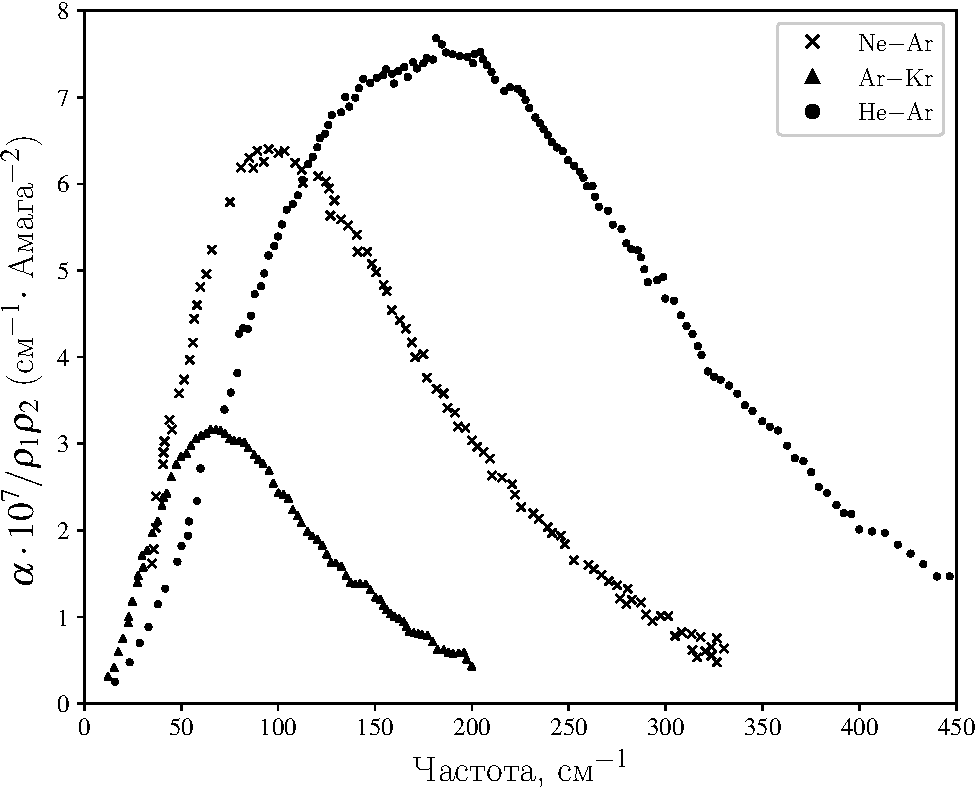
\includegraphics[width=0.7\linewidth]{./pictures/twoatom_experiment/experiment_diatom_spectra-crop.pdf}
    \caption{Экспериментальные спектры бинарного поглощения систем гелий$-$аргон, неон$-$аргон и аргон$-$криптон при комнатной температуре \cite{frommhold}}
    \label{fig:pic-two-atom-experiment}
\end{figure}

В работе \cite{kranendonk1973} авторы разрабатывают формализм расчета столкновительно-индуци\-рован\-ного спектра в приближении бинарных столкновений. Авторы рассматривают систему, состояющую из молекулы H$_2$, взаимодействующей с атомами Ar. Вращательное движение молекулы H$_2$ исключено из рассмотрения -- обе сталкивающихся молекулы рассматриваются как бесструктурные сферически-симметричные частицы. \par
Спектральная функция, определяющая профиль спектра поглощения, связана с функцией автокорреляции суммарного дипольного момента системы преобразованием Фурье \eqref{litreview-spectral-function}. В приближении бинарных столкновений корреляционная функция суммарного дипольного момента принимает вид 
\begin{gather}
    \mean{ \bs{\mu}(0) \bs{\mu}(t) } = N \mean{ \bs{\mu}_1(0) \bs{\mu}_1(t) },
\end{gather} 
%
где через $\bs{\mu_1}(t)$ обозначен дипольный момент, индуцированный квадрупольным полем молекулы H$_2$ на атоме Ar, а $N$ -- количество рассматриваемых пар. Приведенную массу системы авторы обозначают через $\mu$; вектор, соединяющий центр масс молекулы H$_2$ c атомом Ar, -- через $\mathbf{R}$; потенциал взаимодействия -- через $V(R)$ (т.к. вращательное движение молекулы водорода не рассматривается, потенциал зависит только от расстояния между центрами масс $R$). Автокорреляционную функцию дипольного момента приводят к виду 
\begin{gather}
    C(\tau) = \frac{1}{2 \pi} \frac{N}{4 \pi \varepsilon_0} \lb \frac{\mu}{2 \pi k T} \rb^{3/2} \iint \bs{\mu}_1(\mathbf{R}(0)) \cdot \bs{\mu}_1(\mathbf{R}(\tau)) \exp \lb -\frac{\mu \dot{\mf{R}}^2}{2 k T} \rb \zeta(R) \, d \mathbf{R} \, d \dot{\mathbf{R}}, \label{kranendonk-correlation-function}
\end{gather}
%
где $\mathbf{R}(\tau)$ -- значение $\mathbf{R}$, вычисленное в момент времени $\tau$ путем расчета классической траектории, начальными условиями для которой взяты $\mf{R}(0)$ и $\dot{\mf{R}}(0)$, и $\zeta(R)$ -- парная функция распределения 
\begin{gather}
    \zeta(R) = \exp \lb -\frac{V(R)}{kT} \rb.
\end{gather}

Выражение \eqref{kranendonk-correlation-function} неудобно для численного расчета из-за наличия $R(\tau)$ для произвольного момента времени $\tau$. Для более эффективной вычислительной схемы авторы \cite{kranendonk1973} представляют интегральное выражение \eqref{kranendonk-correlation-function} в виде интеграла по полным столкновительным траекториям. При этом будут рассматриваться только траектории рассеяния, связанные состояния исключаются из рассмотрения. В лабораторной системе отсчета энергия система может быть записана в виде
\begin{gather}
    E = \frac{1}{2} \mu \dot{\mf{R}}^2 + V(R).
\end{gather}
Траектория рассеяния, имеющая в момент времени $t$ радиус-вектор $\mf{R}$ и скорость $\dot{\mf{R}}$, однозначно определена относительной скоростью $\mf{g}$ в момент времени $t = -\infty$, прицельным параметром $b$, углом $\varepsilon$, определяющим ориентацию плоскости столковения, и моментом времени $t_0$, в который произошло столкновение. Применяя теорему Лиувилля
\begin{gather}
    d \mf{R} \, d\dot{\mf{R}} = d(t - t_0) b db \, d\varepsilon \, g d\mf{g},
\end{gather}
%
выражение \eqref{kranendonk-correlation-function} преобразуют к виду
\begin{gather}
    C(\tau) = \frac{1}{2 \pi} \frac{N}{4 \pi \varepsilon_0} \lb \frac{\mu}{2 \pi k T} \rb^{3/2} \idotsint \bs{\mu}_1(t) \cdot \bs{\mu}_1(t + \tau) \, \exp \lb - \frac{\mu \mf{g}^2}{2 k T} \rb b \, db \, d\varepsilon \, g d \mf{g} \, dt, \label{correlation-function-kranendonk}
\end{gather}
%
где через $g$ обозначен модуль вектора относительной скорости $\mf{g}$. Используя теорему Винера-Хинчина \cite{frommhold}, авторы \cite{kranendonk1973} получают следующее выражение для спектральной функции 
\begin{gather}
    VJ(\omega) = \frac{1}{2 \pi} \frac{N}{4\pi \varepsilon_0} \lb \frac{\mu}{2 \pi k T} \rb^{3/2} \idotsint \Bigg\vert \intty \bs{\mu}_1(t) e^{-i \omega t} dt \Bigg\vert^2 \, \exp \lb -\frac{\mu g^2}{2 k T} \rb b \, db \, d \varepsilon \, 4 \pi g^3 dg. \label{spectral-function-kranendonk}
\end{gather}

Рассмотрим переход от \eqref{correlation-function-kranendonk} к \eqref{spectral-function-kranendonk} подробно, т.к. мы произведем аналогичное преобразование при выводе альтернативного выражения для спектральной функции в пункте (\ref{section:spectral_function_in_plane}). \par
Корреляцией двух функций $f(z)$ и $g(z)$, определенных на комплексной плоскости $\mathbb{C}$, называют функцию, определенную следующим интегралом
\begin{gather}
    K(z) = \intty f^*(s) g(z + s) ds,
\end{gather}
% 
где $*$ обозначает комплексное сопряжение. Здесь происходит неудачное совпадение названий, т.к. два разных, но близких объекта носят название корреляции. \enquote{Математическую} корреляционную функцию будем обозначать через $K$, а за физическим объектом сохраним обозначение $C$. Обозначим через $F(\omega)$, $G(\omega)$ Фурье-образы функций $f(z)$, $g(z)$. Перепишем выражение для \enquote{математической} корреляции, представив функции через обратное преобразование Фурье от $F(\omega)$, $G(\omega)$, соответственно
\begin{gather}
    K(z) = \intty \lsq \, \intty F^*(\omega) e^{-i \omega s} \frac{d \omega}{2 \pi} \rsq \lsq \, \intty G(\omega^\prime) e^{i \omega^\prime (z + s)} \frac{d\omega^\prime}{2 \pi} \rsq ds.
\end{gather}

Осуществляя перестановку внутри интегрального выражения, приходим к следующему выражению 
\begin{gather}
    K(z) = \frac{1}{2\pi} \intty \intty F^*(\omega) G(\omega^\prime) e^{i \omega^\prime z} \lsq \, \intty e^{i (\omega^\prime - \omega) s} \frac{ds}{2 \pi} \rsq d\omega d\omega^\prime = \notag \\
    = \frac{1}{2\pi} \intty \intty F^*(\omega) G(\omega^\prime) e^{i \omega^\prime z} \delta \lb \omega^\prime - \omega \rb d\omega d\omega^\prime = \hat{F}^{-1} \Big[ F^*(\omega) G(\omega) \Big],
\end{gather}
%
где через $\hat{F}$ обозначен оператор преобразования Фурье. Полученное соотношение, записанное в отношении автокорреляционной функции действительной функции $f$, носит название теоремы Винера-Хинчина \cite{frommhold}
\begin{gather}
    \hat{F} \Big[ K(z) \Big] = \Bigg\vert \hat{F}\Big[ f \Big](\omega) \Bigg\vert^2. 
\end{gather}

Автокорреляционная функция дипольного момента $K(t)$ в подынтегральном выражении \eqref{correlation-function-kranendonk} распадается на сумму автокорреляционных функций $K_\alpha(t)$ компонент дипольного момента 
\begin{gather}
    K(\tau) = \intty \bs{\mu}_1(t) \bs{\mu}_1(t + \tau) dt = \sum_{\alpha = x, y, z} \intty \mu_1^\alpha(t) \mu_1^\alpha(t + \tau) dt = K_x(\tau) + K_y(\tau) + K_z(\tau).
\end{gather}

Следовательно, согласно теореме Винера-Хинчина преобразование Фурье от автокорреляционной функции $K(\tau)$ представляет собой сумму квадратов преобразований Фурье от компонент дипольного момента 
\begin{gather}
    \hat{F}\Big[ K(\tau) \Big] = \sum_{\alpha = x,y,z} \hat{F} \Big[ K_\alpha(\tau) \Big] = \sum_{\alpha=x,y,z} \Bigg\vert \intty \mu_1^\alpha(t) e^{-i\omega t} dt \Bigg\vert^2,
\end{gather}
% 
что для краткости записывают в виде 
\begin{gather}
    \hat{F} \Big[ K(\tau) \Big] = \Bigg\vert \intty \bs{\mu}_1(t) e^{-i\omega t} dt \Bigg\vert^2. \label{correlation-theorem}
\end{gather}

Выражение \eqref{spectral-function-kranendonk} используют при моделировании спектров столкновительно-инду\-ци\-рованного поглощения систем двух атомов методом классических траекторий \cite{levine1967, mcquarrie1968, buryak2014}. Также это выражение можно обобщить на системы, содержащие вращательные степени свободы \cite{oparin2017}. Однако использовать это выражение затруднительно при рассмотрении динамики столкновения в молекулярной системе отсчета, поэтому, используя похожие соображения, мы выведем несколькое иное выражение для спектральной функции для системы двух атомов.

\section{Cистемы координат для описания движения двух атомов} \label{section:two-atom-coordinate-systems}

Рассмотрим движение двух атомов с массами $m_1$, $m_2$ и радиус-векторами $\mf{r}_1$, $\mf{r}_2$ в поле межатомного потенциала $U(\vert \mf{r}_1 - \mf{r}_2 \vert)$. После отделения центра масс задача о движении двух взаимодействующих атомов сводится к задаче о движении виртуальной частицы с приведенной массой $\mu$,  равной 
\begin{gather}
    \mu = \frac{m_1 m_2}{m_1 + m_2}, 
\end{gather}
%
в заданном потенциальном поле $U$ \cite{landau-volume1}. Для описания движения виртуальной частицы введем несколько систем координат. Системой I будем называть декартову систему координат -- положение частицы задается вектором $\mf{r} = \mf{r}_1 - \mf{r}_2$. В этой системе координат лагранжиан и гамильтониан системы записываются как 
\begin{gather}
    \mL_\text{cartesian} = \frac{\mu \dot{\mf{r}}^2}{2} - U( \vert \mf{r} \vert ), \label{two-atom-cartesian-lagrangian} \\
    \mH_\text{cartesian} = \frac{\mf{p}^2}{2\mu} + U( \vert \mf{r} \vert ), \label{two-atom-cartesian-hamiltonian}
\end{gather}
%
где вектор импульса $\mf{p}$ равен
\begin{gather}
    \mf{p} = \frac{\partial \mL_\text{cartesian}}{\partial \dot{\mf{r}}} = \mu \, \dot{\mf{r}}. \label{two-atom-cartesian-momenta}
\end{gather}

Вектор $\mf{r}$ можно представить в сферической системе координат -- длину вектора обозначим через $r$, зенитный и азимутальный углы через $\theta$ и $\varphi$, соответственно ($\theta \in [0, \pi], \varphi \in [0, 2 \pi]$). Будем называть эту координатную систему системой II. Декартовы координаты виртуальной частицы связаны со сферическими координатами следующими соотношениями
\begin{gather}
    \lc
    \begin{aligned}
        x &= r \cos \varphi \sin \theta \\
        y &= r \sin \varphi \sin \theta \\
        z &= r \cos \theta
    \end{aligned}
    \right. \label{two-atom-spherical-coordinates}
\end{gather}

Лагранжиан и гамильтониан в системе координат II записываются как
\begin{gather}
    \mL_\text{spherical} = \frac{1}{2} \mu \dot{r}^2 + \frac{1}{2} \mu r^2 \dot{\theta}^2 + \frac{1}{2} \mu r^2 \dot{\varphi}^2 \sin^2 \theta - U(r),  \label{two-atom-spherical-lagrangian} \\
    \mH_\text{spherical} = \frac{p_r^2}{2 \mu} + \frac{p_\theta^2}{2 \mu r^2} + \frac{p_\varphi^2}{2 \mu r^2 \sin^2 \theta} + U(r), \label{two-atom-spherical-hamiltonian}
\end{gather}
%
где обобщенные импульсы $p_r$, $p_\theta$, $p_\varphi$ связаны с обобщенными скоростями соотношениями
\begin{gather}
    p_r = \frac{\partial \mL_\text{spherical}}{\partial \dot{r}} = \mu \dot{r} \quad \Longrightarrow \quad \dot{r} = \frac{p_r}{\mu}, \label{two-atom-spherical-momenta1} \\
    p_\theta = \frac{\partial \mL_\text{spherical}}{\partial \dot{\theta}} = \mu r^2 \dot{\theta} \quad \Longrightarrow \quad \dot{\theta} = \frac{p_\theta}{\mu r^2}, \label{two-atom-spherical-momenta2} \\
    p_\varphi = \frac{\partial \mL_\text{spherical}}{\partial \dot{\varphi}} = \mu r^2 \dot{\varphi} \sin^2 \theta \quad \Longrightarrow \quad \dot{\varphi} = \frac{p_\varphi}{\mu r^2 \sin^2 \theta}. \label{two-atom-spherical-momenta3}
\end{gather}

Рассмотрим, как связаны декартовы импульсы $\mf{p}$ с импульсами $p_r$, $p_\theta$, $p_\varphi$, сопряженными сферическим координатам. Для этого продифференцируем соотношения \eqref{two-atom-spherical-coordinates} по времени и умножим обе части на приведенную массу $\mu$. Получим в левой части компоненты вектора $\mf{p}$ (согласно \eqref{two-atom-cartesian-momenta}), а в правой части подставим выражения обобщенных скоростей $\dot{r}$, $\dot{\theta}$, $\dot{\varphi}$ через соответствующие импульсы \eqref{two-atom-spherical-momenta1}, \eqref{two-atom-spherical-momenta2}, \eqref{two-atom-spherical-momenta3}
\begin{gather}
    \lc 
    \begin{aligned}
        p_x &= p_r \cos \varphi \sin \theta + \frac{p_\theta}{r} \cos \varphi \cos \theta - \frac{p_\varphi}{r} \frac{\sin \varphi}{\sin \theta}, \\ 
        p_y &= p_r \sin \varphi \sin \theta + \frac{p_\theta}{r} \sin \varphi \cos \theta + \frac{p_\varphi}{r} \frac{\cos \varphi}{\sin \theta}, \\ 
        p_z &= p_r \cos \theta - \frac{p_\theta}{r} \sin \theta.
    \end{aligned}
    \right. \label{two-atom-cartesian-spherical-momenta}
\end{gather}

Разрешая линейные соотношения \eqref{two-atom-cartesian-spherical-momenta} относительно импульсов $p_r$, $p_\theta$, $p_\varphi$, находим соотношения, выражающие обратную связь импульсов
\begin{gather}
    \lc
    \begin{aligned}
        p_r &= r \lb p_x \cos \varphi \sin \theta + p_y \sin \varphi \sin \theta + p_z \cos \theta \rb, \\
        p_\varphi &= r \sin \theta \lb p_y \cos \varphi - p_x \sin \varphi \rb, \\
        p_\theta &= r \lb p_x \cos \varphi \cos \theta + p_y \sin \varphi \cos \theta - p_z \sin \theta \rb.  
    \end{aligned}
    \right.
\end{gather}

Выразим компоненты углового момента через координаты и импульсы системы II, пользуясь соотношениями \eqref{two-atom-cartesian-spherical-momenta}
\begin{gather}
    \mf{J} = \lsq \mf{r} \times \mf{p} \rsq = 
    \begin{bmatrix}
        -p_\theta \sin \varphi - p_\varphi \cos \varphi \cot \theta \\
        -p_\varphi \sin \varphi \cot \theta + p_\theta \cos \varphi \\
        p_\varphi
    \end{bmatrix}. \label{two-atom-angular-momenta-spherical} 
\end{gather}

Известно, что в отсутствии внешнего момента сил угловой момент является векторным интегралом движения, следовательно движение двух атомов происходит в перпендикулярной ему плоскости \cite{goldstein}. Для описания динамики системы введем полярные координаты $r, \psi$ и соответствующие обобщенные скорости $\dot{r}$, $\dot{\psi}$. Ориентацию плоскости будем задавать при помощи пары сферических углов $\Phi$, $\Theta$, описывающих направление вектора углового момента. Определим систему координат таким образом, чтобы координатная плоскость $OXY$ совпадала с плоскостью движения, а ось $OZ$ была сонаправлена с вектором углового момента $\mf{J}$. Будет называть эту координатную систему системой III; лагранжиан и гамильтониан в ней равны 
\begin{gather}
    \mL_\text{plane} = \frac{1}{2} \mu \dot{r}^2 + \frac{1}{2} \mu r^2 \dot{\psi}^2 - U(r), \label{two-atom-plane-lagrangian} \\
    \mH_\text{plane} = \frac{p_r^2}{2\mu} + \frac{p_\psi^2}{2 \mu r^2} + U(r), \label{two-atom-plane-hamiltonian} 
\end{gather}
%
где обобщенные импульсы $p_r$, $p_\psi$ связаны с обобщенными скоростями следующими соотношениями
\begin{gather}
    p_r = \frac{\partial \mL_\text{plane}}{\partial \dot{r}} = \mu \dot{r} \quad \Longrightarrow \quad \dot{r} = \frac{p_r}{\mu}, \label{two-atom-plane-momenta1} \\
    p_\psi = \frac{\partial \mL_\text{plane}}{\partial \dot{\psi}} = \mu r^2 \dot{\psi} \quad \Longrightarrow \quad \dot{\psi} = \frac{p_\psi}{\mu r^2}.  \label{two-atom-plane-momenta2}
\end{gather}

Перевод полярных координат $r$, $\psi$ системы III в декартовы координаты $\mf{r} = \lc x, y, z \rc$ системы I можно осуществить при помощи ортогональной матрицы вращения $\bbS$, параметризованной углами $\Phi$, $\Theta$ \cite{goldstein} 
\begin{gather}
    \begin{bmatrix}
        x \\ y \\ z
    \end{bmatrix} 
    = \bbS_\Phi^{-1} \bbS_\Theta^{-1} 
    \begin{bmatrix}
        r \cos \psi \\ r \sin \psi \\ 0
    \end{bmatrix}, \label{two-atoms-coordinate-transformation}
\end{gather}
% 
где матрицы поворота $\bbS_\Phi$, $\bbS_\Theta$ равны
\begin{gather}
    \bbS_\Phi = 
    \begin{bmatrix}
       -\sin \Phi & \cos \Phi & 0 \\
       -\cos \Phi & -\sin \Phi & 0 \\
      0 & 0 & 1
    \end{bmatrix}, \quad
    \bbS_\Theta = 
    \begin{bmatrix}
        1 & 0 & 0 \\
        0 & \cos \Theta & \sin \Theta \\
        0 & -\sin \Theta & \cos \Theta
    \end{bmatrix}.
\end{gather}

Раскрывая матричное выражение \eqref{two-atoms-coordinate-transformation}, получаем 
\begin{gather}
    \left\{
        \begin{aligned}
            x &= -r \cos \psi \sin \Phi - r \sin \psi \cos \Phi \cos \Theta \\
            y &= r \cos \psi \cos \Phi - r \sin \psi \sin \Phi \cos \Theta \\
            z &= r \sin \psi \sin \Theta
        \end{aligned}
    \right. \label{two-atoms-coordinates-transformation2}
\end{gather}

Продифференцируем соотношения \eqref{two-atoms-coordinates-transformation2} по времени, учитывая, что углы $\Phi$, $\Theta$ от времени не зависят.
\begin{gather}
    \begin{bmatrix} \dot{x} \\ \dot{y} \\ \dot{z} \end{bmatrix} = 
    \bbS_\Phi^{-1} \bbS_\Theta^{-1}
    \begin{bmatrix} 
        \dot{r} \cos \psi - r \dot{\psi} \sin \psi \\
        \dot{r} \sin \psi + r \dot{\psi} \cos \psi \\
        0 
    \end{bmatrix} \\
    \lc
    \begin{aligned}
        \dot{x} &= - \dot{r} \lb \cos \psi \sin \Phi + \sin \psi \cos \Phi \cos \Theta \rb + r \dot{\psi} \lb \sin \psi \sin \Phi - \cos \psi \cos \Phi \cos \Theta \rb \\ 
        \dot{y} &= \dot{r} \lb \cos \psi \cos \Phi - \sin \psi \sin \Phi \sin \Theta \rb - r \dot{\psi} \lb \sin \psi \cos \Phi - \cos \psi \sin \Phi \cos \Theta \rb \\
        \dot{z} &= \dot{r} \sin \psi \sin \Theta + r \dot{\psi} \cos \psi \sin \Theta
    \end{aligned}
\right. \label{two-atoms-coordinates-transformation3}
\end{gather}

При рассмотрении средних значений функций по фазовому пространству нам понадобятся выражения импульсов $\mf{p}$ через импульсы $p_r$, $p_\psi$. При умножении левых частей соотношений \eqref{two-atoms-coordinates-transformation3} на приведенную массу $\mu$ мы получим компоненты вектора $\mf{p}$ (согласно \eqref{two-atom-cartesian-momenta}). Подставив выражения обобщенных скоростей $\dot{r}$, $\dot{\psi}$ через импульсы $p_r$, $p_\psi$ (\eqref{two-atom-plane-momenta1}, \eqref{two-atom-plane-momenta2}), получаем
\begin{gather}
    \lc
    \begin{aligned}
        p_x &= -p_r \lb \sin \psi \cos \Phi \cos \Theta + \cos \psi \sin \Phi \rb + \frac{p_\psi}{r} \lb \sin \psi \sin \Phi - \cos \psi \cos \Phi \cos \Theta \rb \\
        p_y &= p_r \lb \cos \psi \cos \Phi - \sin \psi \sin \Phi \cos \Theta \rb - \frac{p_\psi}{r} \lb \sin \psi \cos \Phi + \cos \psi \sin \Phi \cos \Theta \rb \\
        p_z &= p_r \sin \psi \sin \Theta + \frac{p_\psi}{r} \cos \psi \sin \Theta 
    \end{aligned}
\right. \label{two-atom-momenta-transformation}
\end{gather}

Выразим компоненты углового момента через координаты системы III, исходя из определения вектора углового момента 
\begin{gather}
    \mf{J} = \mu \lsq \mf{r} \times \dot{\mf{r}} \rsq = 
    \begin{bmatrix}
        \mu r^2 \dot{\psi} \cos \Phi \sin \Theta \\ 
        \mu r^2 \dot{\psi} \sin \Phi \sin \Theta \\
        \mu r^2 \dot{\psi} \cos \Theta
    \end{bmatrix},
\end{gather}
или, пользуясь соотношением между скоростью $\dot{\psi}$ и импульсом $p_\psi$ \eqref{two-atom-plane-momenta2}, 
\begin{gather}
    \mf{J} = 
    \begin{bmatrix}
        p_\psi \cos \Phi \sin \Theta \\
        p_\psi \sin \Phi \sin \Theta \\
        p_\psi \cos \Theta
    \end{bmatrix}. \label{two-atom-plane-angular-momenta}
\end{gather}

Выражение \eqref{two-atom-plane-angular-momenta} показывает, что углы $\Phi$, $\Theta$ являются сферическими углами для вектора углового момента. Кроме того, замечаем, что импульс $p_\psi$ имеет физический смысл модуля вектора углового момента. 

\section{Усреднение функций по фазовому пространству в разных системах координат} \label{section:averaging}

Рассмотрим усреднение некоторой функции $f(\mf{r}, \mf{p})$ по фазовому пространству двухатомной системы, где $\mf{r}$, $\mf{p}$ -- векторы декартовых координат и сопряженных импульсов (система I): 
\begin{gather}
    \mean{f} = \idotsint f(\mf{r}, \mf{p}) \exp \lb -\frac{\mH(\mf{r},\mf{p})}{kT} \rb d \mf{r} \, d\mf{p}. \label{two-atom-mean}
\end{gather}

Целью нашего рассмотрения будет отыскание выражений, позволяющих производить усреднение функции $f$ по фазовому пространству, пользуясь координатами систем II и III. \par
Рассмотрим совокупную систему уравнений \eqref{two-atoms-coordinates-transformation2}, \eqref{two-atom-momenta-transformation} и найдем якобиан замены переменных $\lc x, y, z, p_x, p_y, p_z \rc$ $\rightarrow$ $\lc r, p_r, \psi, p_\psi, \Phi, \Theta \rc$. Ввиду громоздкости выкладки приводить не будем, выражение для якобиана получается следующее:
\begin{gather}
    \text{Jac} = \Bigg\vert \frac{\partial \lsq x, y, z, p_x, p_y, p_z \rsq}{\partial \lsq r, p_r, \psi, p_\psi, \Phi, \Theta \rsq} \Bigg\vert = p_\psi \sin \Theta. \label{two-atom-planar-jacobian}
\end{gather}

Итак, среднее значение \eqref{two-atom-mean} в системе координат III записывается как
\begin{gather}
    \mean{ f } = \int\limits_{0}^{\infty} dr \intty dp_r \int\limits_0^{2\pi} d\psi \int\limits_0^\infty p_\psi dp_\psi \int\limits_0^\pi \sin \Theta d\Theta \int\limits_0^{2\pi} d\Phi f(r, \psi, p_r, p_\psi, \Theta, \Phi) \exp \lb -\frac{\mH_\text{plane}}{k T} \rb. \label{two-atom-mean-plane1} 
\end{gather}

Если усредняемая функция $f(r, \psi, p_r, p_\psi, \Theta, \Phi)$ не зависит от углов $\Theta$, $\Phi$, то среднее значение  \eqref{two-atom-mean-plane1} принимает вид 
\begin{gather}
    \mean{ f } = 4 \pi \int\limits_{0}^{\infty} dr \intty dp_r \int\limits_0^{2\pi} d\psi \int\limits_0^\infty p_\psi dp_\psi f(r, \psi, p_r, p_\psi, \Theta, \Phi) \exp \lb -\frac{\mH_\text{plane}}{k T} \rb. \label{two-atom-mean-plane2} 
\end{gather}

Как уже отмечалось ранее, импульс $p_\psi$ имеет физический смысл модуля углового момента, поэтому область интегрирования этого импульса составляет полуось $(0, +\infty)$, в то время как для радиального импульса -- вся прямая $(-\infty, +\infty)$. \par
Аналогично, рассмотрим совокупную систему уравнений \eqref{two-atom-spherical-coordinates}, \eqref{two-atom-cartesian-spherical-momenta} и найдем якобиан замены переменных $\lc x, y, z, p_x, p_y, p_z \rc$ $\rightarrow$ $\lc r, p_r, \varphi, p_\varphi, \theta, p_\theta \rc$. Якобиан оказывается единичным: 
\begin{gather}
    \text{Jac} = \Bigg\vert \frac{\partial \lsq x, y, z, p_x, p_y, p_z \rsq}{\partial \lsq r, p_r, \varphi, p_\varphi, \theta, p_\theta \rsq} \Bigg\vert = 1. 
\end{gather}

Таким образом, среднее значение \eqref{two-atom-mean} в системе координат II записывается как
\begin{gather}
    \mean{f} = \int\limits_0^\infty dr \intty dp_r \int\limits_0^{2\pi} d\varphi \intty dp_\varphi \int\limits_0^\pi d\theta \intty dp_\theta f(r, p_r, \varphi, p_\varphi, \theta, p_\theta) \exp \lb -\frac{\mH_\text{spherical}}{k T} \rb. \label{two-atom-mean-spherical}
\end{gather}

\section{Распределения координат и импульсов в фазовом пространстве в разных системах координат} \label{section:two-atom-distributions} 

Рассмотрим вопрос распределения координат и импульсов в фазовом пространстве в системах координат II и III в условиях канонического ансамбля. Функция распределения в фазовом пространстве в условиях канонического ансамбля задана гамильтонианом системы $\mH$ \cite{hill} 
\begin{gather}
    \rho \lb \mf{q}, \mf{p} \rb = \Gamma_0 \exp \lb -\frac{\mH \lb \mf{q}, \mf{p} \rb}{\kb T} \rb,
\end{gather}
% 
где постоянная $\Gamma_0$ определяется из условия нормировки функции распределения
\begin{gather}
    \int \rho \lb \mf{q}, \mf{p} \rb d \mf{q} \, d\mf{p} = 1.
\end{gather}

Рассмотрим распределения угловых координат $\theta, \varphi$ и импульсов $p_r$, $p_\theta$, $p_\varphi$ системы II при фиксированном большом значении межатомного расстояния $r_\text{fixed} \gg 1$. Пренебрежем значением потенциала $U(r_\text{fixed}) \approx 0$ на расстоянии $r_\text{fixed}$ (для системы He$-$Ar было использовано фиксированное межатомное расстояние, равное $\rfixed = 40 a_0$, где через $a_0$ обозначен Боровский радиус). Удобно представить отношение $\mH / \kb T$ в виде трех квадратичных членов $\lc \frac{1}{2} x_j^2 \rc_{j = 1 \dots 3}$
\begin{gather}
    \frac{\mH_\text{spherical}}{\kb T} = \frac{p_r^2}{2 \mu \kb T} + \frac{p_\theta^2}{2 \mu r_\text{fixed}^2 \kb T} + \frac{p_\varphi^2}{2 \mu r_\text{fixed}^2 \kb T \sin^2 \theta} = \frac{1}{2} x_1^2 + \frac{1}{2} x_2^2 + \frac{1}{2} x_3^2, \label{two-atom-spherical-hamiltonian-xs} 
\end{gather}
%
где переменные $x_j$ выражены как
\begin{gather}
    \lc
    \begin{aligned}
        x_1 &= \frac{p_r}{\sqrt{\mu \kb T}}, \\
        x_2 &= \frac{p_\theta}{\sqrt{\mu r_\text{fixed}^2 \kb T}}, \\
        x_3 &= \frac{p_\varphi}{\sqrt{\mu r_\text{fixed}^2 \kb T \sin^2 \theta}}.
    \end{aligned}
\right. \label{two-atom-xs}
\end{gather}

Переписав гамильтониан в виде \eqref{two-atom-spherical-hamiltonian-xs}, мы видим, что вероятность нахождения системы в элементе фазового объема $d\theta d\varphi dx_1 dx_2 dx_3$ пропорциональна произведению 
\begin{gather}
    \rho \lb \theta, \varphi, x_1, x_2, x_3 \rb \propto \rho_1(x_1) \rho_1(x_2) \rho_1(x_3) \sin \theta, \label{two-atom-xs-phase-element}
\end{gather}
%
где случайные величины $x_j$ распределены по нормальному закону
\begin{gather}
    \rho_1 (x_j) = \frac{1}{\sqrt{2 \pi}} \exp \lb -\frac{x_j^2}{2} \rb. 
\end{gather}

Соотношения \eqref{two-atom-xs} позволяют установить следующие функции распределения для двух импульсов
\begin{gather}
    \lc
    \begin{aligned}
        p_r &\sim \mN \lb 0, \mu \kb T \rb, \\
        p_\theta &\sim \mN \lb 0, \mu r_\text{fixed}^2 \kb T \rb, 
    \end{aligned}
    \right.
\end{gather}
%
где через $\mN \lb \mu, \sigma^2 \rb$ обозначено нормальное распределение с математическим ожиданием $\mu$ и дисперсией $\sigma^2$. Импульс $p_\varphi$ представляет собой произведение двух случайных величин
\begin{gather}
    p_\varphi = x_3 \cdot \sin \Theta, \label{two-atom-pvarphi-generation}
\end{gather}
% 
где величина $x_3$ распределена по нормальному закону $\mN \lb 0, \mu r_\text{fixed}^2 \kb T \rb$, а плотность распределения случайной величины $\Theta$ в силу \eqref{two-atom-xs-phase-element} равна
\begin{gather}
    \rho(\Theta) = \frac{1}{2} \sin \Theta.
\end{gather}

Численная генерация случайных величин $p_\varphi$ легко осуществляется по выражению \eqref{two-atom-pvarphi-generation}, однако интересно получить аналитическое выражение для плотности распределения, так как такие же распределения возникают при рассмотрении импульсов в многоатомных комплексах. Сначала получим плотность распределения величины $\sin \Theta$, используя то, что $\cos \Theta$ распределен равномерно на отрезке $\lsq -1, 1\rsq$. Очевидно, что в области определения зенитного угла $\lsq 0, \pi \rsq$ знак $\sin \Theta$ определен однозначно, следовательно выбираем положительный знак корня 
\begin{gather}
    \sin \Theta = \sqrt{ 1 - \cos^2 \Theta}.
\end{gather}
Далее воспользуемся формулой преобразования случайной величины $Y = g(X)$
\begin{gather}
    \rho_Y(y) = \Big\vert \frac{d}{dy} g^{-1}(y) \Big\vert \cdot \rho_X(g^{-1}(y)), \label{distribution-change}
\end{gather}
%
где через $\rho_X(x)$, $\rho_Y(y)$ обозначены плотности случайных величин $X$, $Y$, соответственно. В данном случае преобразование осуществляется функцией $g(x) = \sqrt{1 - x^2}$, подстановка которой в \eqref{distribution-change} приводит к следующей плотности распределения для $\sin \Theta$ 
\begin{gather}
    \rho_{\sin \Theta}(x) = \frac{x}{\sqrt{1 - x^2}} \cdot \bbI\lsq 0, 1\rsq,
\end{gather}
% 
где через $\bbI\lsq 0, 1 \rsq$ обозначена индикаторная функция, ограничивающая носитель функции отрезком $\lsq 0, 1 \rsq$. Отметим, что полученное распределение является частным случаем распределения Кумарасвами с параметрами $a = 2$, $b = 1/2$ \cite{kumaraswamy1980}. \par
Плотность распределения $\rho_{p_\varphi}$ может быть получена по стандартной формуле плотности случайной величины, являющейся произведением двух других случайных величин
\begin{gather}
    \rho_{p_\varphi}(z) = \intty \rho_{x_3}(z/x) \rho_{\sin \Theta}(x) \frac{dx}{\vert x \vert}.
\end{gather}
Подставив явные выражения для плотностей распределения, получаем следующий интеграл
\begin{gather}
    \rho_{p_\varphi}(z) = \frac{1}{\sqrt{2 \pi}} \int\limits_0^1 \frac{\displaystyle \exp \lb -\frac{z^2}{2x^2} \rb}{\sqrt{1 - x^2}} dx,
\end{gather}
%
разрешив который приходим к
\begin{gather}
    \rho_{p_\varphi}(z) = \frac{\pi}{8} \lb 1 - \text{sgn}(z) \text{erf} \lb \frac{z}{\sqrt{2}} \rb \rb.
\end{gather}
Так как угол $\varphi$ не входит в гамильтониан $\mH_\text{spherical}$, то он распределен с равномерной плотностью на отрезке $\lsq 0, 2 \pi \rsq$.

\setcounter{figure}{1}
\begin{figure}[H]
    \centering
    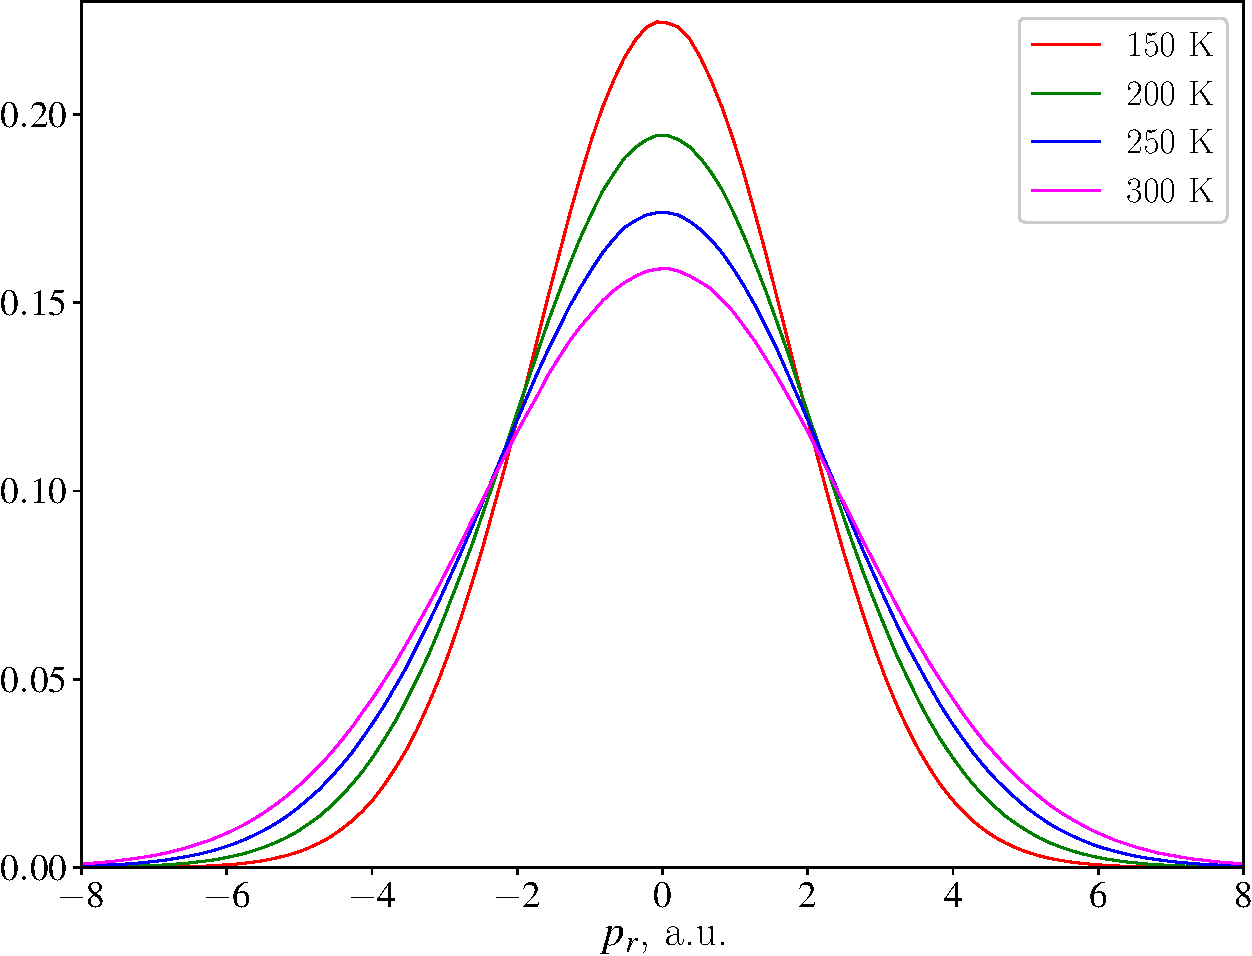
\includegraphics[width=0.75\linewidth]{./pictures/two_atom_distributions/pR-crop.pdf} \\
    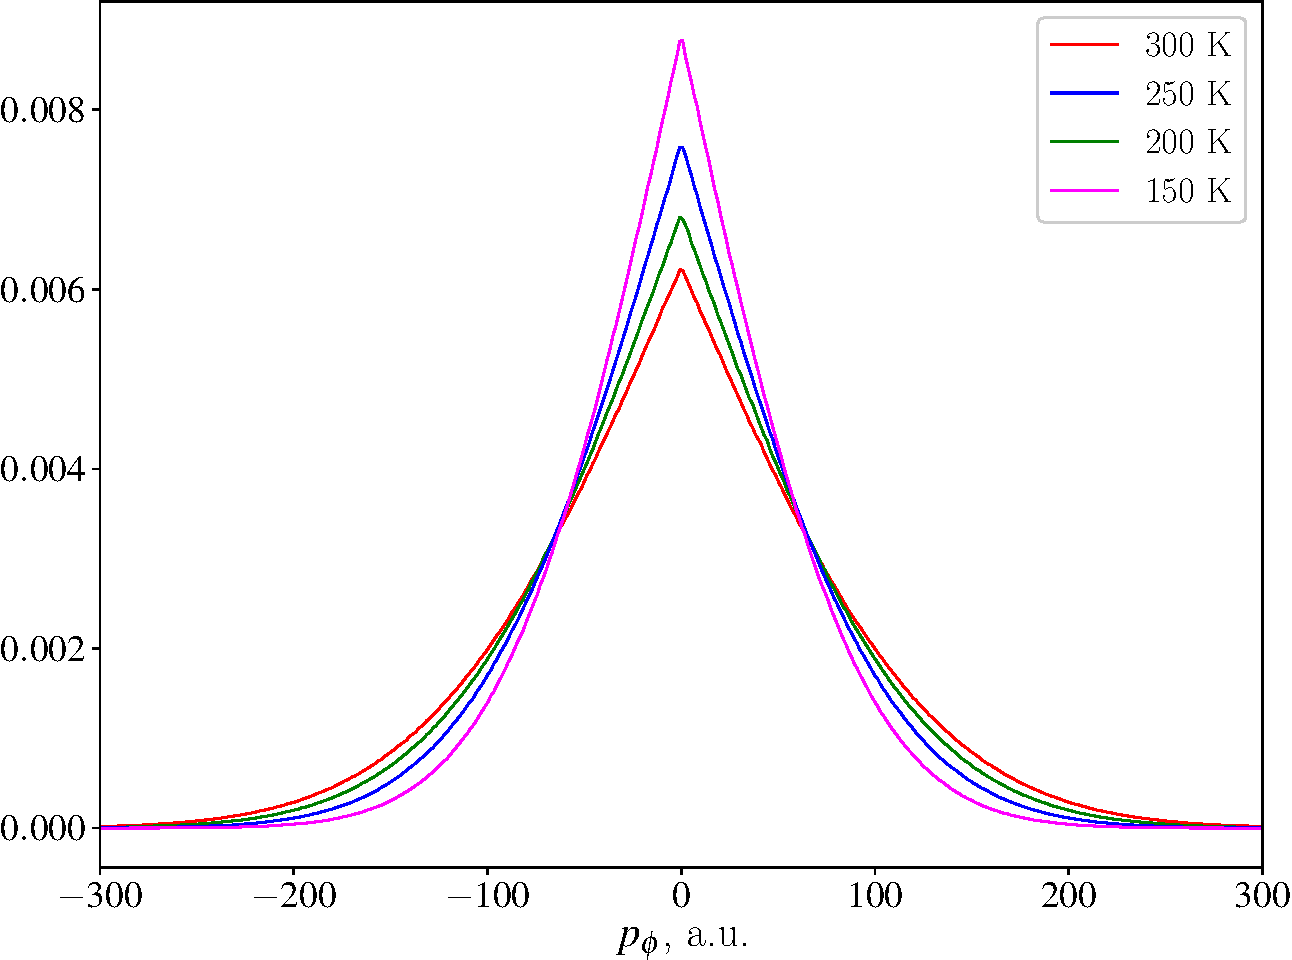
\includegraphics[width=0.75\linewidth]{./pictures/two_atom_distributions/pPhi-crop.pdf}
    \caption{Плотности распределений импульсов $p_r$ и $p_\varphi$ при температурах от 150K до 300K с шагом 50K для системы He$-$Ar. Максимумы плотностей распределений убывают с увеличением температуры. Межатомное расстояние $r_\text{fixed}$ взято равным $40 a_0$. Количество сгенерированных точек при каждой температуре -- $N = 5 \cdot 10^7$.}
    \label{fig:pr-pphi-distributions}
\end{figure}

Если переходить теперь к переменным системы координат III, то легко заметить, что плотность распределения импульса $p_r$ совпадает с той, что была получена в системе координат II. Угол $\psi$ не входит в гамильтониан, следовательно распределен с равномерной плотностью. Так как якобиан замены декартовых координат и импульсов на координаты и импульсы системы III равен $p_\psi \sin \Theta$ (соотношение \eqref{two-atom-planar-jacobian}), то получаем, что плотность распределения импульса $p_\psi$ пропорциональна
\begin{gather}
    \rho(p_\psi) \propto p_\psi \exp \lb -\frac{p_\psi^2}{2 \mu r_\text{fixed}^2 \kb T} \rb, \label{two-atom-ppsi-distribution}
\end{gather}
где коэффициент пропорциональности устанавливается из условия нормировки и оказывается равным $1/(\mu r_\text{fixed}^2 \kb T)$. Из вида якобиана \eqref{two-atom-planar-jacobian} вытекает, что угол $\Theta$ распределен равномерно с косинусом. \par
Распределение для импульса $p_\psi$ может быть установлено и из других соображений. Как уже отмечалось, $p_\psi$ имеет физический смысл модуля углового момента $\mf{J}$. Исходя из выражения \eqref{two-atom-angular-momenta-spherical}, получаем, что квадрат модуля углового момента $J^2$ связан с импульсами $p_\varphi$, $p_\theta$ соотношением
\begin{gather}
    J^2 = p_\psi^2 = p_\theta^2 + \frac{p_\varphi^2}{\sin^2 \theta}. \label{two-atom-angular-momenta-connection} 
\end{gather}
Мы уже установили, что величины $p_\theta$ и $p_\varphi / \sin \theta$ распределены согласно нормальному закону. Квадраты нормально распределенных случайных величин распределены согласно хи-квадрат распределению с одной степенью свободы $\chi_1^2$ \cite{castaneda}. А сумма двух одномерных хи-квадрат распределений $\chi_1^2$ дает двумерное хи-квадрат распределение $\chi_2^2$. Наконец, для того чтобы получить распределение величины $p_\psi$, извлекаем корень из двумерного хи-квадрат распределения $\chi_2^2$ и получаем двумерное хи-распределение $\chi_2$, известное как распределение Рэлея, плотность которого задается  
\begin{gather}
    \rho(x; \sigma) = \frac{x}{\sigma^2} \exp \lb -\frac{x^2}{2 \sigma^2} \rb. \label{rayleigh-density}
\end{gather}

Выражение \eqref{two-atom-ppsi-distribution} является частным случаем распределением Рэлея с параметром $\sigma^2 = \mu r_\text{fixed}^2 \kb T$.

\setcounter{figure}{2}
\begin{figure}[H]
    \centering
    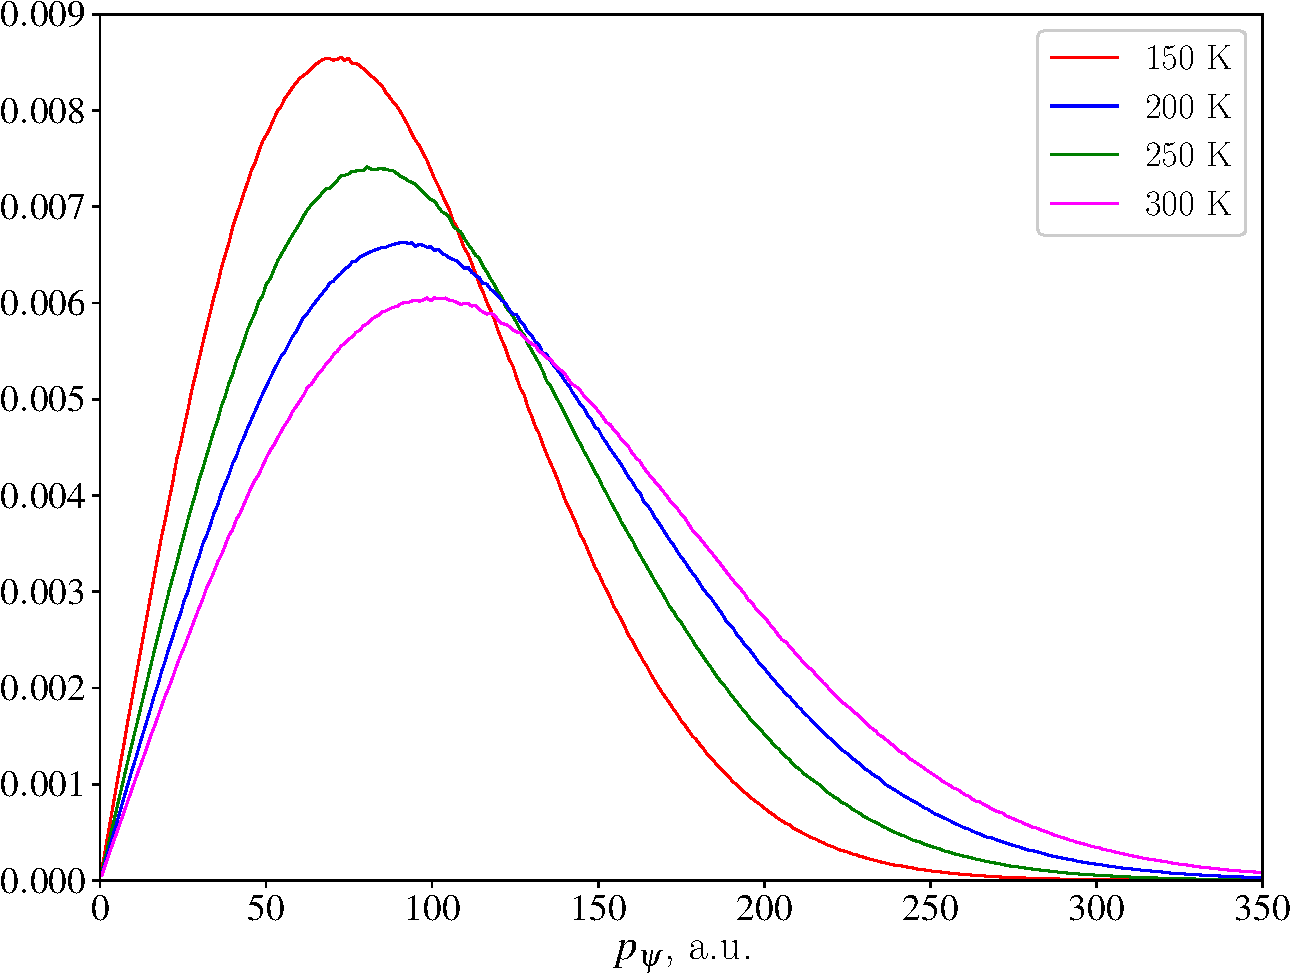
\includegraphics[width=0.75\linewidth]{./pictures/two_atom_distributions/pPsi-crop.pdf}
    \caption{Плотности распределений импульса $p_\psi$ при температурах от 150К до 300К с шагом 50К для системы He$-$Ar. Максимумы распределений уменьшаются и сдвигаются вправо с уменьшением температуры. Межатомное расстояние $r_\text{fixed}$ было взято равным $40a_0$. Количество сгенерированных точек при каждой температуре -- $N = 5 \cdot 10^7$.}
    \label{fig:ppsi-distributions}
\end{figure}

\section{Спектральная функция при рассмотрении динамики столкновения в плоскости} \label{section:spectral_function_in_plane}

Рассмотрим произведение спектральной функции на объем, являющееся преобразованием Фурье от автокорреляционной функции дипольного момента согласно \eqref{litreview-autocorrelation-function-definition}   
\begin{gather}
    VJ(\omega) = \frac{1}{2 \pi} \frac{V}{4 \pi \varepsilon_0} \intty \mean{ \bs{\mu}(0) \bs{\mu}(t) } e^{-i \omega t} dt.
\end{gather}

Мы будем пользоваться приближением бинарных столкновений, то есть будем предполагать, что суммарная автокорреляционная функция распадается на сумму автокорреляционных функций индуцированных диполей пар. Для индуцированного дипольного момента пары мы сохраним для простоты  обозначение $\bs{\mu}$. Итак, мы будем работать со следующим выражением для спектральной функции с трактовкой интеграла как интеграла по начальным условиям классических динамических траекторий, как обсуждалось в пункте \ref{section:correlation_functions} 
\begin{gather}
    VJ(\omega) = \frac{1}{2\pi} \frac{V}{4 \pi \varepsilon_0} \intty \frac{\displaystyle \idotsint \bs{\mu}(0) \bs{\mu}(t) \, \exp \lb -\frac{\mH}{kT} \rb d\mf{q} \, d\mf{p}}{\displaystyle \idotsint \exp \lb -\frac{\mH}{kT} \rb d\mf{q} \, d\mf{p}} e^{-i \omega t} dt. \label{two-atom-spectral-function1}
\end{gather}

Вектор координат при рассмотрении в плоскости столкновений равен $\mf{q} = \lc r, \psi, \Phi, \Theta \rc$, а вектор импульсов -- $\mf{p} = \lc p_r, p_\psi \rc$. Кроме того, согласно пункту \ref{section:averaging} в интеграле появляется дополнительный весовой множитель, равный $\text{Jac} = p_\psi \sin \Theta$. Следовательно, полное интегральное выражение в этой системе координат выглядит следующим образом
\begin{gather}
    VJ(\omega) = \frac{1}{2\pi} \frac{V}{4 \pi \varepsilon_0} \intty e^{-i\omega t} dt \frac{\displaystyle \int\limits_0^\infty dr \intty dp_r \int\limits_0^{2\pi} d\psi \int\limits_0^\infty p_\psi dp_\psi \int\limits_0^\pi \sin \Theta d\Theta \int\limits_0^{2\pi} d\Phi \bs{\mu}(0) \bs{\mu}(t) \exp \lb -\frac{\mH_\text{plane}}{kT} \rb}{\displaystyle \int\limits_0^\infty dr \intty dp_r \int\limits_0^{2\pi} d\psi \int\limits_0^\infty p_\psi dp_\psi \int\limits_0^\pi \sin \Theta d\Theta \int\limits_0^{2\pi} d\Phi \exp \lb -\frac{\mH_\text{plane}}{kT} \rb}. \label{two-atom-spectral-function2}
\end{gather}

Заметим, что скалярное произведение дипольных моментов $\bs{\mu}(0) \bs{\mu}(t)$ и гамильтониан $\mH$ не зависят от углов $\Phi$, $\Theta$. Проинтегрировав по ним, мы получаем множитель $4 \pi$ как в числителе, так и знаменателе, поэтому суммарно никаких дополнительных множителей не возникает.
\begin{gather}
    VJ(\omega) = \frac{1}{2 \pi} \frac{V}{4 \pi \varepsilon_0} \intty e^{-i\omega t} dt \frac{\displaystyle \int\limits_0^\infty dr \intty dp_r \int\limits_0^{2\pi} d\psi \int\limits_0^\infty p_\psi dp_\psi \bs{\mu}(0) \bs{\mu}(t) \exp \lb -\frac{\mH_\text{plane}}{kT} \rb}{\displaystyle \int\limits_0^\infty dr \intty dp_r \int\limits_0^{2\pi} d\psi \int\limits_0^\infty p_\psi dp_\psi \exp \lb -\frac{\mH_\text{plane}}{kT} \rb}. \label{two-atom-spectral-function3}
\end{gather}

Как известно, решение задачи о движении частицы с приведенной массой $\mu$ в центральном поле можно получить, основываясь на законах сохранения энергии и углового момента в интегральном виде \cite{landau-volume1}. Гамильтониан, записанный в полярных координатах, определенных в плоскости движения (система III), 
\begin{gather}
    \mH_\text{plane} = \frac{p_r^2}{2\mu} + \frac{p_\psi^2}{2\mu r^2} + U(r) = E,
\end{gather}
%
является интегралом движения. Импульс $p_\psi$ также является интегралом движения. Решение уравнений движения в интегральном виде выглядит следующим образом \cite{landau-volume1} 
\begin{gather}
    t = \int\limits_{r_\text{нач}}^{r} \frac{dr}{\displaystyle \sqrt{\frac{2}{\mu} \lb E - U(r) \rb - \frac{p_\psi^2}{\mu^2 r^2}}}, \label{two-atom-change1} \\
    \psi = \int\limits_{r_\text{нач}}^{r} \frac{\displaystyle \frac{p_\psi}{r^2} dr}{\displaystyle \sqrt{2\mu \lb E - U(r) \rb - \frac{p_\psi^2}{r^2}}}, \label{two-atom-change2}
\end{gather}
где $r_\text{нач}$ -- начальное значение межатомного расстояния, а $r$ -- межатомное расстояние в момент времени $t$.  

Рассмотрим замену координат в интеграле в числителе \eqref{two-atom-spectral-function3} следующего вида
\begin{gather}
    \lc r, p_r, \psi, p_\psi \rc \rightarrow \lc (\rfixed), \tau, p_r^\prime, \psi^\prime, p_\psi \rc \label{two-atom-change-variables-time}.
\end{gather}

Физический смысл этой замены координат состоит в том, что вместо того чтобы начинать классическую траекторию с произвольного межатомного расстояния $r$, мы хотим использовать фиксированное начальное расстояние $\rfixed$ ($\rfixed$ взят в скобках, потому что фиксирован для всех траекторий). Переменная $\tau$ задает время, за которое межатомное расстояние становится равным $r$. Если взять исходное $\rfixed$ бесконечно большим, то набор переменных $\lc \tau, p_r^\prime, \psi^\prime, p_\psi \rc$ опишет тот же массив свободно-разлетных траекторий, что и набор переменных $\lc r, p_r, \psi, p_\psi \rc$. Понятно, что в интеграле \eqref{two-atom-spectral-function3} нам нужно перечислить лишь те классические траектории, на которых межатомное расстояние уменьшилось до такой степени, что появился значительный индуцированный дипольный момент. Поэтому, если мы положим $\rfixed$ больше некоторого расстояния, за которым мы считаем индуцированный дипольный момент равным нулю, то мы перечислим весь значимый массив траекторий (классические траектории, для которых минимальное сближение между атомами больше $\rfixed$, не будут тогда учтены в интеграле, но и интегральный вклад от них равен нулю). Подходящее расстояние $\rfixed$ следует подбирать на основании радиальной зависимости индуцированного дипольного момента для каждой конкретной системы по-своему. Импульс $p_\psi$ сохраняется при описанной замене. \par
Для оговоренного набора траекторий замена переменных \eqref{two-atom-change-variables-time} является взаимоднозначной в силу единственности решения задачи Коши. \par
Заметим, что интегральные выражения \eqref{two-atom-change1}, \eqref{two-atom-change2} описывают ровно половину классической траектории -- от $\rfixed$ до поворотной точки $r_0$, определяемой уравнением
\begin{gather}
    \frac{2}{\mu} \lb E - V(r_0) - \frac{p_\psi^2}{2 \mu r_0^2} \rb = 0.
\end{gather}
Классические траектории столкновения двух тел являются симметричными относительно поворотной точки \cite{goldstein}, поэтому мы без ограничения общности можем рассматривать только ту половину траектории, в ходе которой происходит разлет двух тел от поворотной точки $r_0$ до некоторого выбранного значения $\rfixed$. Другими словами, будем рассматривать такие наборы начальных условий $\lc r, p_r, \psi, p_\psi \rc$,  в которых импульсы $p_r$ являются положительными, и будем сопоставлять им наборы начальных условий $\lc \tau, p_r^\prime, \psi^\prime, p_\psi \rc$, в которых импульсы $p_r^\prime$ также являются положительными величинами. \par
Итак, координаты $\tau$, $p_r^\prime$, $\psi^\prime$ связаны с исходными $r$, $p_r$, $\psi$ следующими соотношениями
\begin{gather}
    \lc
    \begin{aligned}
        \tau &= \int\limits_r^{\rfixed} \frac{dr^\prime}{\displaystyle \sqrt{\frac{2}{\mu} \lb E - U(r^\prime) - \frac{p_\psi^2}{2 \mu r^{\prime 2}} \rb}}, \\
        \psi^\prime &= \psi + \int\limits_r^{\rfixed} \frac{\displaystyle \frac{p_\psi}{r^{\prime 2}} dr^\prime}{\displaystyle \sqrt{2\mu \lb E - U(r^\prime) - \frac{p_\psi^2}{2 \mu r^{\prime 2}} \rb}}, \\
        p_r^\prime &= \sqrt{2 \mu \lb E - \frac{p_\psi^2}{2 \mu \rfixed^2} - U(\rfixed) \rb},
    \end{aligned}
    \right. \label{two-atom-change3}
\end{gather}
%
где последнее соотношение получено исходя из закона сохранении энергии в форме
\begin{gather}
    E = \frac{p_r^2}{2\mu} + \frac{p_\psi^2}{2 \mu r^2} + U(r) = \frac{p_r^{\prime 2}}{2 \mu} + \frac{p_\psi^2}{2 \mu \rfixed^2} + U(\rfixed). 
\end{gather}

Учитывая в какой форме записаны соотношения \eqref{two-atom-change3}, найдем якобиан $\displaystyle \Bigg\vert \frac{\partial \lsq \tau, p_r^\prime, \psi^\prime, p_\psi \rsq}{\partial \lsq r, p_r, \psi, p_\psi \rsq} \Bigg \vert$, а затем, пользуясь тем, что якобианы обратны друг к другу
\begin{gather}
    \Bigg\vert \frac{\partial \lsq \tau, p_r^\prime, \psi^\prime, p_\psi \rsq}{\partial \lsq r, p_r, \psi, p_\psi \rsq} \Bigg \vert \cdot \Bigg\vert \frac{\partial \lsq r, p_r, \psi, p_\psi \rsq}{\partial \lsq \tau, p_r^\prime, \psi^\prime, p_\psi \rsq} \Bigg \vert = 1,
\end{gather}
%
найдем интересующий нас якобиан
\begin{gather}
    \text{Jac} = \Bigg\vert \frac{\partial \lsq r, p_r, \psi, p_\psi \rsq}{ \partial \lsq \tau, p_r^\prime, \psi^\prime, p_\psi \rsq} \Bigg\vert.
\end{gather}

Итак, якобиан $\text{Jac}^{-1}$ имеет следующую структуру
\begin{gather}
    \text{Jac}^{-1} =
    \det
    \begin{bdmatrix}
        \frac{\partial \tau}{\partial r} & \frac{\partial \tau}{\partial p_r} & \frac{\partial \tau}{\partial \psi} & \frac{\partial p_\psi}{\partial r} \\
        \frac{\partial p_r^\prime}{\partial r} & \frac{\partial p_r^\prime}{\partial p_r} & \frac{\partial p_r^\prime}{\partial \psi} & \frac{\partial p_r^\prime}{\partial p_\psi} \\
        \frac{\partial \psi^\prime}{\partial r} & \frac{\partial \psi^\prime}{\partial p_r} & \frac{\partial \psi^\prime}{\partial \psi} & \frac{\partial \psi^\prime}{\partial p_\psi} \\
        \frac{\partial p_\psi}{\partial r} & \frac{\partial p_\psi}{\partial p_r} & \frac{\partial p_\psi}{\partial \psi} & \frac{\partial p_\psi}{\partial p_\psi} 
    \end{bdmatrix} = 
    \begin{vmatrix}
        a & b & 0 & c \\
        d & e & 0 & f \\
        g & h & 1 & k \\
        0 & 0 & 0 & 1
    \end{vmatrix}.
\end{gather}

Все производные по $\psi$, за исключением $\partial \psi^\prime / \partial \psi$, равны 0, т.к. $\psi$ не входит в выражения для соответствующих переменных. Производная же $\partial \psi^\prime / \partial \psi$ равна 1, потому что $\psi$ только аддитивно входит в выражение для $\psi^\prime$.
Переменная $p_\psi$ остается неизменной в результате замены, поэтому последняя строчка матрицы оказывается такой простой. \par
Вследствие особенностей структуры якобиана, получается, что $\text{Jac}^{-1}$ зависит только от 4 элементов
\begin{gather}
    \text{Jac}^{-1} = a \cdot e - b \cdot d.  
\end{gather}

Явные выражения для этих элементов матрицы выглядят следующим образом 
\begin{gather}
    a = \frac{\partial \tau}{\partial r} = -\frac{\mu}{p_r} - \frac{1}{\mu} \lb \frac{dU}{dr} - \frac{p_\psi^2}{\mu r^3} \rb \cdot I_1, \\ 
    b = \frac{\partial \tau}{\partial p_r} = - \frac{p_r}{\mu^2} I_1, \\ 
    d = \frac{\partial p_r^\prime}{\partial r} = \frac{\displaystyle \mu \lb \frac{dU}{dr} - \frac{p_\psi^2}{\mu r^3} \rb}{\displaystyle \sqrt{2\mu \lb E - \frac{p_\psi^2}{2 \mu \rfixed^2} - U(\rfixed) \rb}} = \frac{\mu}{p_r^\prime} \lb \frac{dU}{dr} - \frac{p_\psi^2}{\mu r^3} \rb, \\
    e = \frac{\partial p_r^\prime}{\partial p_r} = \frac{p_r}{\displaystyle \sqrt{2\mu \lb E - \frac{p_\psi^2}{2 \mu \rfixed^2} - U(\rfixed) \rb}} = \frac{p_r}{p_r^\prime},
\end{gather}
%
где введено обозначение 
\begin{gather}
    I_1 = \int\limits_r^{\rfixed} \lsq \frac{2}{\mu} \lb E - U(r^\prime) - \frac{p_\psi^2}{2 \mu r^{\prime 2}} \rb \rsq^{-3/2} dr^\prime. 
\end{gather}

Для полноты представим остальные элементы якобиана
\begin{gather}
    c = \frac{\partial \tau}{\partial p_\psi} = -\frac{p_\psi}{\mu} \int\limits_r^{\rfixed} \lb \frac{1}{r^2} - \frac{1}{r^{\prime 2}} \rb \lsq \frac{2}{\mu} \lb E - U(r^\prime) - \frac{p_\psi^2}{2 \mu r^{\prime 2}} \rb \rsq^{-3/2} dr^\prime \\
f = \frac{\partial p_r^\prime}{\partial p_\psi} = \frac{\displaystyle p_\psi \lb \frac{1}{r^2} - \frac{1}{\rfixed^2} \rb}{\displaystyle \sqrt{2 \mu \lb E - \frac{p_\psi^2}{2 \mu \rfixed^2} - U(\rfixed) \rb}} = \frac{p_\psi}{p_r^\prime} \lb \frac{1}{r^2} - \frac{1}{\rfixed^2} \rb \\
    g = \frac{\partial \psi^\prime}{\partial r} = -\frac{p_\psi}{p_r r^2} - \mu p_\psi \lb \frac{dU}{dr} - \frac{p_\psi^2}{\mu r^3} \rb I_2, \\ 
    h = \frac{\partial \psi^\prime}{\partial p_r} = -p_\psi p_r \cdot I_2, \\ 
    k = \frac{\partial \psi^\prime}{\partial p_\psi} = \int\limits_r^{\rfixed} \frac{1}{r^{\prime 2}} \lsq 2 \mu \lb E - U(r^\prime) - \frac{p_\psi^2}{2 \mu r^2} \rb \rsq \lsq 2 \mu \lb E - U(r^\prime) - \frac{p_\psi^2}{2 \mu r^{\prime 2}} \rb\rsq^{-3/2} dr^\prime,
\end{gather}
%
где было введено обозначение
\begin{gather}
    I_2 = \int\limits_r^{\rfixed} \frac{dr^\prime}{r^{\prime 2}} \lsq 2 \mu \lb E - U(r^\prime) - \frac{p_\psi^2}{2 \mu r^{\prime 2}} \rb \rsq^{-3/2}.
\end{gather}

Итак, якобианы оказываются равными
\begin{gather}
    \Bigg\vert \frac{\partial \lsq \tau, p_r^\prime, \psi^\prime, p_\psi \rsq}{\partial \lsq r, p_r, \psi, p_\psi \rsq} \Bigg\vert = \frac{\mu}{p_r^\prime}, \quad \Bigg\vert \frac{\partial \lsq r, p_r, \psi, p_\psi \rsq}{\partial \lsq \tau, p_r^\prime, \psi^\prime, p_\psi \rsq} \Bigg\vert = \frac{p_r^\prime}{\mu}.
\end{gather}

Следовательно, выражение для спектральной функции \eqref{two-atom-spectral-function3} может быть переписано в виде
\begin{gather}
    VJ(\omega) = \frac{1}{2 \pi \Gamma_0} \frac{V}{4 \pi \varepsilon_0} \intty e^{-i \omega t} dt \int\limits_0^\infty d\tau \intty \frac{p_r^\prime}{\mu} dp_r^\prime \int\limits_0^{2\pi} d\psi^\prime \int\limits_0^\infty p_\psi dp_\psi \bs{\mu}(0) \bs{\mu}(\tau) \exp \lb -\frac{\mH_\text{plane}}{kT} \rb,
\end{gather}
%
где через $\Gamma_0$ обозначен интеграл, находящийся в знаменателе \eqref{two-atom-spectral-function3}
\begin{gather}
    \Gamma_0 = \int\limits_0^\infty dr \intty dp_r \int\limits_0^{2\pi} d\psi \int\limits_0^\infty p_\psi dp_\psi \exp \lb -\frac{\mH_\text{plane}}{kT} \rb.
\end{gather}

Переставив интеграл по времени $t$ c интегралами по переменным $\tau$, $p_r^\prime$, $\psi^\prime$ и $p_\psi$, воспользуемся корреляционной теоремой \eqref{correlation-theorem}
\begin{gather}
    VJ(\omega) = \frac{1}{2 \pi \Gamma_0} \frac{V}{4 \pi \varepsilon_0} \int\limits_0^\infty \frac{p_r^\prime}{\mu} dp_r^\prime \int\limits_0^{2\pi} d\psi^\prime \int\limits_0^\infty p_\psi dp_\psi \Bigg\vert \intty \bs{\mu}(t) e^{-i \omega t} dt \Bigg\vert^2 \exp \lb -\frac{\mH_\text{plane}}{k T} \rb. \label{two-atom-spectral-function4}
\end{gather}

Итак, выражение для спектральной функции \eqref{two-atom-spectral-function4} является аналогом выражения \eqref{spectral-function-kranendonk} при рассмотрении динамики в гамильтоновых переменных в плоскости столкновения. В следующем параграфе будут приведены результаты расчетов спектральных функций и профилей по выражению \eqref{two-atom-spectral-function4}. Рассмотрение систем типа атом$-$линейная молекула и пара линейных молекул, описанное в следующей главе, опирается на обобщение выведенного выражения для спектральной функции. 

\iffalse
Integral ratio:
\begin{gather}
    \int \exp \lb -\frac{T_H}{kT} \rb d \psi d p_r dp_\psi = 2 \pi^2 \mu k T r \\
    \int \exp \lb -\frac{T_H}{kT} \rb dr d\psi dp_r dp_\psi = \pi^2 \mu k T r^2 \\
    \frac{\int \exp \lb -\frac{T_H}{kT} \rb d\psi dp_r dp_\psi}{\int \exp \lb -\frac{T_H}{k T} \rb dr d\psi dp_r dp_\psi} = \frac{2}{r}
\end{gather}
\fi

\section{Трансляционные спектры газовой смеси He$-$Ar}

Экспериментальные исследования газовых смесей инертных газов He$-$Ar и Ne$-$Ar проводились в работах \cite{bosomworth1965_part1, bosomworth1965_part2} при околокомнатных температурах. Полученные в более ранней работе \cite{kiss1959} данные ограничены спектральным диапазоном от 350 до 700 см$^{-1}$ и плохо согласуются с более подробными данными, представленными в \cite{bosomworth1965_part2}, поэтому при комнатной температуре сравнение теоретического спектрального профиля мы будем проводить с данными из \cite{bosomworth1965_part2}. Трансляционные спектры систем He$-$Ar и Ne$-$Ar при низких температурах экспериментально исследовались в работах \cite{bukhtoyarova1977, bukhtoyarova1977_2, ryzhov1974}. \par 
Исторически при моделировании трансляционных спектров благородных газов авторы пользовались модельными поверхностями потенциальной энергии и дипольного момента. В работе \cite{levine1967} авторы рассматривают прямолинейные классические траектории столкновения в отсутствие межатомного потенциала; в качестве модели функции дипольного момента была взята гауссова функция, которая совершенно не воспроизводит физического поведения дипольного момента, однако позволяет проводить аналитические выкладки. Сделанные приближения позволили получить аналитическое выражение для коэффициента поглощения $\alpha(\omega)$ с использованием спецфункций. В результате подгонки параметров функции дипольного момента аналитическая модель для коэффициента поглощения была согласована с экспериментальными данными. \par
В работе \cite{mcquarrie1968} представлено моделирование столкновительно-индуцированного спектра методом классических траекторий. Авторы использовали потенциал Леннарда-Джонса (6, 12) с параметрами, подогнанными под экспериментальные данные о сечениях рассеяния. Зависимость дипольного момента от расстояния аппроксимировалась экспоненциальной функцией в области малых межатомных расстояний; при больших расстояниях предполагалось, что дипольный момент отсутствует. При помощи подгонки коэффициента, определяющего скорость спада функции дипольного момента от расстояния, авторам удалось неплохо согласовать свои результаты с экспериментальными данными \cite{bosomworth1965_part2}. \par
Работа \cite{sharma1975} посвящена моделированию столкновительно-индуцированного спектра в рамках квантового формализма. Авторы использовали функции дипольного момента, построенные на основе дальнодействующей компоненты с радиальной асимптотикой $r^{-7}$ и короткодействующей компоненты, растущей экспоненциально с уменьшением расстояния. Качество используемых поверхностей потенциальной энергии и дипольного момента не позволило достичь высокого уровня согласия с экспериментальными данными. \par
Работа \cite{meyer1986} является одной из самых ранних работ, в которой была получена \textit{ab initio} поверхность дипольного момента и использована при расчете спектральной функции $J(\omega)$ в рамках квантового формализма. Расчеты дипольного момента проводились методами Хартри-Фока и конфигурационного взаимодействия в серии базисных наборов. Полученные расчетные значения дипольного момента были аппроксимированы простой аналитической функцией. Отклонение спектральной функции от экспериментальных данных не превышает 10\%. \par 
С развитием современных квантовохимических методов поверхности потенциальной энергии и дипольного момента смесей благородных газов были подробно изучены многими авторами \cite{cybulski1999, giece2003, fernandez2004}. Расчеты производились с использованием методов CCSD/CCSD(T) в корреляционно-согласованных базисных наборах, дополненных связевыми функциями, расположенными на равном расстоянии от обоих атомов. В наиболее современной работе \cite{fernandez2004} авторы использовали метод CCSD(T) и базисный набор aug-cc-pV6Z-33211 для расчета поверхности потенциальной энергии, и CCSD/d-aug-cc-pVQZ-33211 -- для расчета поверхности дипольного момента. Для оценки точности поверхности потенциальной энергии авторы рассчитали температурную зависимость смешанного вириального коэффициента $B_{12}(T)$. Авторы \cite{fernandez2004} отмечают, что полученные ими поверхности находятся практически в полном согласии с данными \cite{cybulski1999}. В наших расчетах мы использовали предложенные в \cite{fernandez2004} аналитические разложения поверхностей потенциальной энергии и дипольного момента. \par
В работе \cite{buryak2014} было проведено сравнение траекторного и квантового подходов к расчету трансляционных спектров систем He$-$Ar и Ne$-$Ar. При сравнении использовались поверхности потенциальной энергии \cite{fernandez2004} и дипольного момента \cite{fernandez2004, meyer1986}. Теоретически спектральные профили, полученные в квантовом формализме, должны лучше описывать экспериментальные данные. Авторы показывают, что результаты, полученные в классическом траекторном расчете, оказываются в хорошем согласии как с квантовыми расчетами, так и с экспериментальными данными. Было отмечено, что некоторую проблему при классическом моделировании спектра представляет собой процедура десимметризации профиля, которую мы рассмотрим позже. \par

\section{Вычислительные аспекты расчета столкновительно$-$инду\-цированного спектра методом классических траекторий}

Расчет спектральной функции системы из двух атомов в нашей работе мы будем производить по выражению \eqref{two-atom-spectral-function4}. Вычисление многомерного интеграла будем производить методом Монте-Карло, т.к. при рассмотрении систем с большим количеством вращательных степеней свободы мы столкнемся с интегралами значительно более высокой размерности, вычисление которых квадратурными методами не представляется возможным. В данном случае при интегрировании квадратурами общие вычислительные затраты могут оказаться меньше, однако такая схема интегрирования не может быть перенесена на системы, в которых мономеры обладают несколькими вращательными степенями свободы, поэтому мы отказались от ее реализации. Известно, что погрешность метода Монте-Карло асимптотически ведет себя как $N^{-1/2}$, где $N$ -- количество точек, по которым производилась оценка интеграла \cite{sobol}. Такая асимптотика ошибки не позволяет получать очень точных оценок интегралов, что в некоторых задачах оказывается неудовлетворительным. В задаче моделирования континуального спектрального профиля точность порядка $\sim 0.5\%$ приемлема, что достижимо с использованием метода Монте-Карло. Более подробно вопрос о точности получающегося спектрального профиля в нашем подходе мы обсудим после описания вычислительной схемы. \par
Интегрирование в \eqref{two-atom-spectral-function4} мы будем производить методом Монте-Карло с весовой функцией $p_\xi(\bxi) = p_\psi \exp \lb -\mH_\text{plane}(\bxi) / \kb T \rb / \Gamma_1$, где $\bxi = \lc p_r^\prime, \psi^\prime, p_\psi \rc$, а $\Gamma_1$ -- нормировочный множитель, равный
\begin{gather}
    \Gamma_1 = \int\limits_0^\infty dp_r^\prime \intty d\psi^\prime \intty p_\psi \exp \lb -\frac{\mHplane}{\kb T} \rb dp_\psi.
\end{gather}
Выражение \eqref{two-atom-spectral-function4} может быть рассмотрено как математическое ожидание квадрата преобразования Фурье на распределении $\boldsymbol{\xi}$
\begin{gather}
    V J(\omega) = \frac{V}{4 \pi \varepsilon_0} \frac{\Gamma_1}{2 \pi \Gamma_0} \lim_{N \rightarrow \infty} \frac{1}{N} \sum_{k = 1}^N \frac{p_r^\prime(\bxi_k)}{\mu} \Bigg\vert \intty \bs{\mu}(t; \bxi_k) e^{-i \omega t} dt \Bigg\vert^2, \label{two-atom-spectral-function-mc}
\end{gather}
%
где обозначение $p_r^\prime(\bxi_k)$ подразумевает, что импульс, сопряженный радиальной координате, взят из вектора $\bxi$, реализующего распределение с плотностью $p_\xi$. \par
Основываясь на выкладках, сделанных в параграфе \ref{section:averaging}, несложно получить аналитические выражения для интегралов $\Gamma_0, \Gamma_1$
\begin{gather}
    \Gamma_0 = \int\limits_0^\infty dr \intty dp_r \int\limits_0^{2\pi} d\psi \int\limits_0^\infty p_\psi \exp \lb -\frac{\mHplane}{\kb T} \rb d p_\psi = \frac{4}{3} \pi r_\text{fixed}^3 \lb 2 \pi \mu \kb T \rb^{3/2}, \\
    \Gamma_1 = \int\limits_0^\infty dp_r \int\limits_0^{2\pi} d\psi \int\limits_0^\infty p_\psi \exp \lb -\frac{\mHplane}{\kb T} \rb dp_\psi  = 2 \pi r_\text{fixed}^2 \lb 2 \pi \mu \kb T \rb^{3/2}.
\end{gather}
Таким образом, конечное выражение для спектральной функции, как среднее значение на распределении с плотностью $p_\xi(\bxi)$, принимает вид 
\begin{gather}
    VJ(\omega) = \frac{\rfixed^2}{4 \pi \varepsilon_0} \lim_{N \rightarrow \infty} \frac{1}{N} \sum_{k = 1}^N \frac{p_r^\prime(\bxi_k)}{\mu} \Big\vert \intty \bs{\mu}(t; \bxi_k) e^{i \omega t} dt \Big\vert^2. \label{two-atom-spectral-function-mc-final}
\end{gather}

Вопрос генерации реализаций случайной величины $\bxi$ с плотностью распределения $p_\xi$ обсуждался в параграфе \ref{section:averaging}. Рассмотрим вопрос расчета классических траекторий рассеяния. Несмотря на то что для динамических переменных могут быть выписаны квадратурные выражения, которыми мы пользовались в параграфе \ref{section:spectral_function_in_plane}, вычисления по ним производить не очень удобно. В первую очередь неудобство связано с тем, что для вычисления усредняемого выражения в \eqref{two-atom-spectral-function-mc-final} нам потребуется вычислять преобразование Фурье от дипольного момента вдоль траектории, которое эффективно реализуется в виде дискретного преобразования Фурье. Для этого нам потребуются значения дипольного момента $\bs{\mu}(t)$ с равномерным шагом по времени, что вызовет некоторые затруднения при вычислениях по квадратурной формуле. Кроме того, квадратуры для всех динамических переменных являются несобственными интегралами, имеющими особенность в поворотной точке. Поэтому траектории рассеяния рассчитывались интегрированием трех уравнений Гамильтона
\begin{gather}
    \lc
    \begin{aligned}
        \dot{r} &= \frac{p_r}{\mu} \\
        \dot{\psi} &= \frac{p_\psi^2}{\mu r^3} - \frac{d U}{d r} \\
        \dot{p_\psi} &= \frac{p_\psi}{\mu r^2}
    \end{aligned}
    \right. \label{two-atom-hamilton-equations}
\end{gather}

Была разработана программа на языке С++, реализующая классический траекторный расчет по описанной схеме. Система уравнений \eqref{two-atom-hamilton-equations} численно интегрировалась при помощи пакета процедур для решения дифференциальных уравнений SUNDIALS \cite{sundials}. Использовались процедуры, реализующие так называемые разностные формулы назад (bacward differentiation formulate -- BDF) \cite{curtiss1952} переменного порядка, используемые при решении \enquote{жестких} систем дифференциальных уравнений. Решение нелинейных уравнений, возникающих в результате применения BDF формул, происходит с использованием стандартного метода Ньютона. Вычисления производились с двойной точностью со значением параметра, определяющего относительную ошибку решения, равным $10^{-15}$. Так как каждая траектория может быть рассчитана независимо от остальных, то была написана программа для расчета массива траекторий в параллельном режиме. В коде была использована библиотека MPI \cite{mpi}, стандартизующая передачу сообщений между узлами параллельного приложения. Приложение реализовано в модели взаимодействия \enquote{ведущий-ведомый}, в которой \enquote{ведущий} процесс отвечает за распределение начальных условий между \enquote{ведомыми} процессами, осуществляющими расчет траекторий. Получив начальное условие, \enquote{ведомый} процесс рассчитывает траекторию рассеяния с внутренним переменным шагом по времени, при этом с фиксированным шагом по времени $\Delta t = 200$ атомных единиц времени (около 5 фс) вдоль траектории вычисляется значение индуцированного дипольного момента и собирается в заранее подготовленный массив, содержащий $L = 2^{15}$ ячеек. Расчет траектории заканчивается в тот момент, когда межатомное расстояние вновь достигает начального значения или количество вычислений дипольного момента превышает $L$. Затем в рамках \enquote{ведомого} процесса осуществляется дискретное преобразование Фурье временной зависимости индуцированного дипольного момента. Выбор длины массива $L$ обусловлен тем, что наиболее эффективно дискретное преобразование Фурье выполняется для массива, длина которого есть некоторая степень двух (так называемое быстрое преобразование Фурье). Согласно выражению \eqref{two-atom-spectral-function-mc-final} вычисляется квадрат преобразования Фурье (трактовка вычисления квадрата обсуждалась в самом начале главы \ref{chapter:two-atom}), умножается на отношение радиального импульса $p_r$ в начальный момент времени к приведенной массе $\mu$, и полученный массив передается на \enquote{ведущий} процесс. \enquote{Ведущий} процесc накапливает результаты \enquote{ведомых} процессов и после усреднения получает спектральную функцию.
    Спектральный профиль, полученный в результате траекторного расчета, представлен на рис. \ref{fig:two-atom-desymmetrizations}.
\setcounter{figure}{3}
\begin{figure}
    \centering
    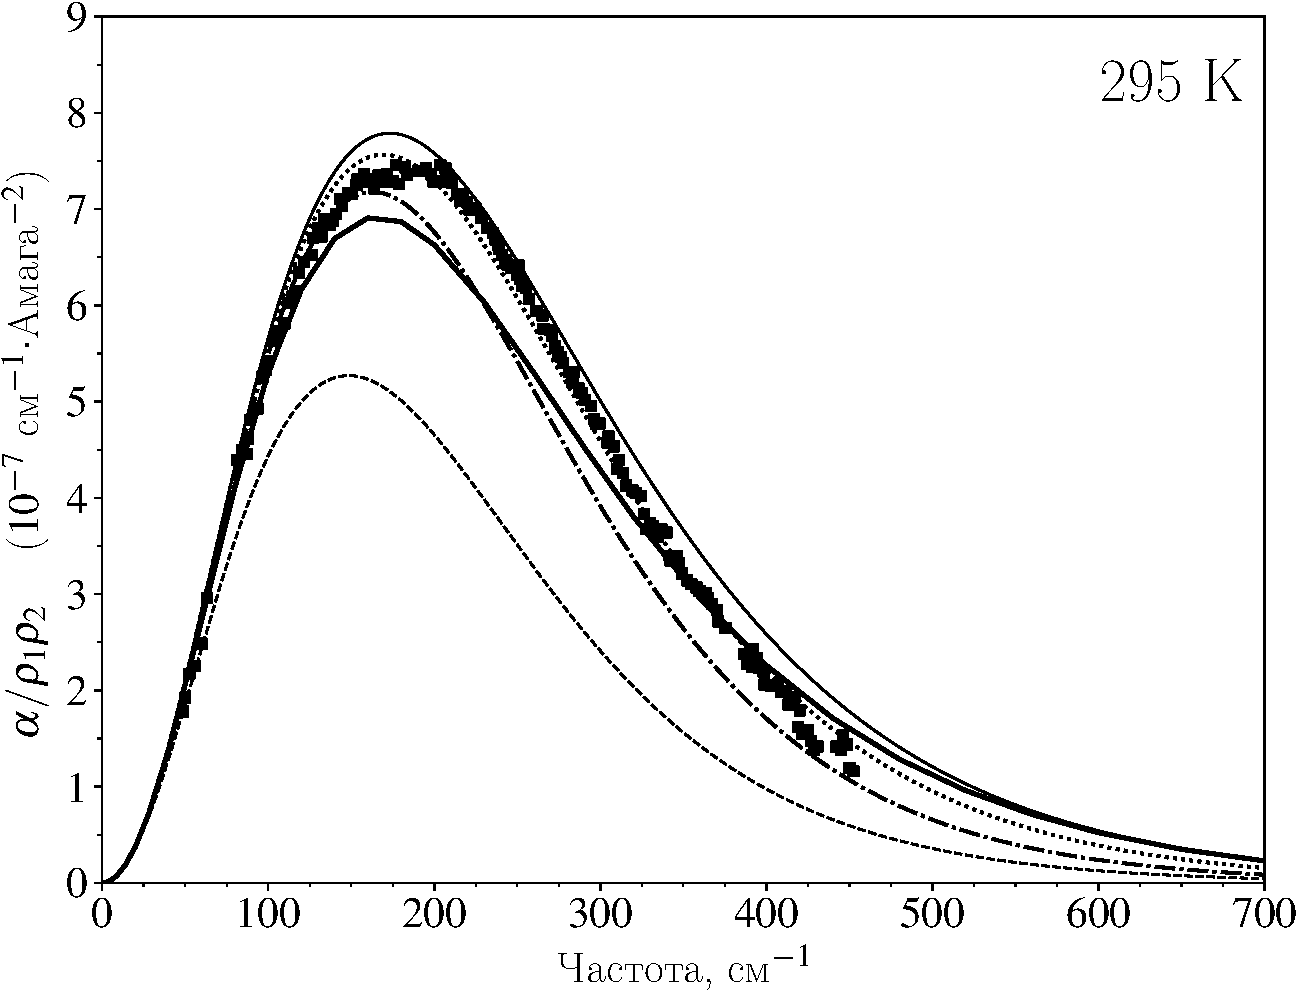
\includegraphics[width=0.7\linewidth]{./pictures/two_atom_spectra/desymmetrizations_295K-crop.pdf}
    \caption{Сравнение классического и квантового спектральных профилей для системы He$-$Ar с профилями, полученными в результате применения различных процедур десимметризации. Пунктиром обозначен классический профиль, сплошной толстой линией -- квантовый профиль \cite{buryak2014}, точками с пунктиром -- профиль, полученный в результате применения процедуры D1, точечной линией -- профиль, полученный в результате применения процедуры D2, сплошной линией -- профиль, полученный в результате применения процедуры D3. Квадратами обозначены экспериментальные данные \cite{bosomworth1965_part2}.}
    \label{fig:two-atom-desymmetrizations}
\end{figure}

Как известно, классические траектории обратимы во времени. Это свойство классических траекторий приводит к тому, что автокорреляционная функция дипольного момента $C(t)$ является симметричной функцией от времени \cite{frommhold}
\begin{gather}
    C(t) = C(-t).
\end{gather}

Классическая спектральная функция, получающаяся в результате применения преобразования Фурье к автокорреляционной функции, также оказывается симметричной функции частоты 
\begin{gather}
    J_\text{class.}(\omega) = J_\text{class.}(-\omega). \label{classical-detailed-balance}
\end{gather}

Однако квантовая спектральная функция удовлетворяет так называемому условию детального баланса \cite{frommhold} 
\begin{gather}
    J(-\omega) = J(\omega) \exp \lb -\frac{\hbar \omega}{\kb T} \rb, \label{detailed-balance}
\end{gather}
%
которое может быть получено из выражения \eqref{part1-spectral-function-definition} перестановкой индексов $j, k$. Условие детального баланса \eqref{detailed-balance} отражает разницу в заселенностях исходного и конечного состояний. Соотношение \eqref{classical-detailed-balance} называют классическим условием детального баланса. \par
Считается, что симметрийная разница между классической и квантовой спектральной функциями может быть устранена при помощи так называемой процедуры десимметризации. Предполагается, что классическую спектральную функцию можно определенным образом \enquote{десимметризовать} так, что функция, получившаяся в результате, будет удовлетворять квантовому условию детального баланса \cite{borysow1985phenomena}. Однако процедура десимметризации не может быть однозначна задана условием детального баланса: можно построить бесконечное количество процедур, которые будут приводить к спектральной функции, удовлетворяющей квантовому условию детального баланса \cite{frommhold}. Поэтому от процедуры десимметризации дополнительно требуют совпадения десимметризованного классического профиля с квантовым профилем -- в области дальних крыльев в особенности. \par
В литературе представлен набор различных процедур десимметризации \cite{borysow1985}. Некоторые из них устроены следующим образом:
\begin{gather}
    J_{D1}(\omega) = \frac{2}{1 + \exp \lb -\hbar \omega / \kb T \rb} J_\text{class}(\omega)  \\
    J_{D2}(\omega) = \frac{\hbar \omega}{\kb T} \frac{1}{1 - \exp \lb -\hbar \omega / \kb T \rb} J_\text{class}(\omega) \\
    J_{D3}(\omega) = \exp \lb \frac{\hbar \omega}{2 \kb T} \rb J_\text{class}(\omega)
\end{gather}
В литературе также используется преобразование Эгельстаффа \cite{egelstaff1962}; в настоящей работе мы его не использовали. 

\begin{figure}
    \centering
    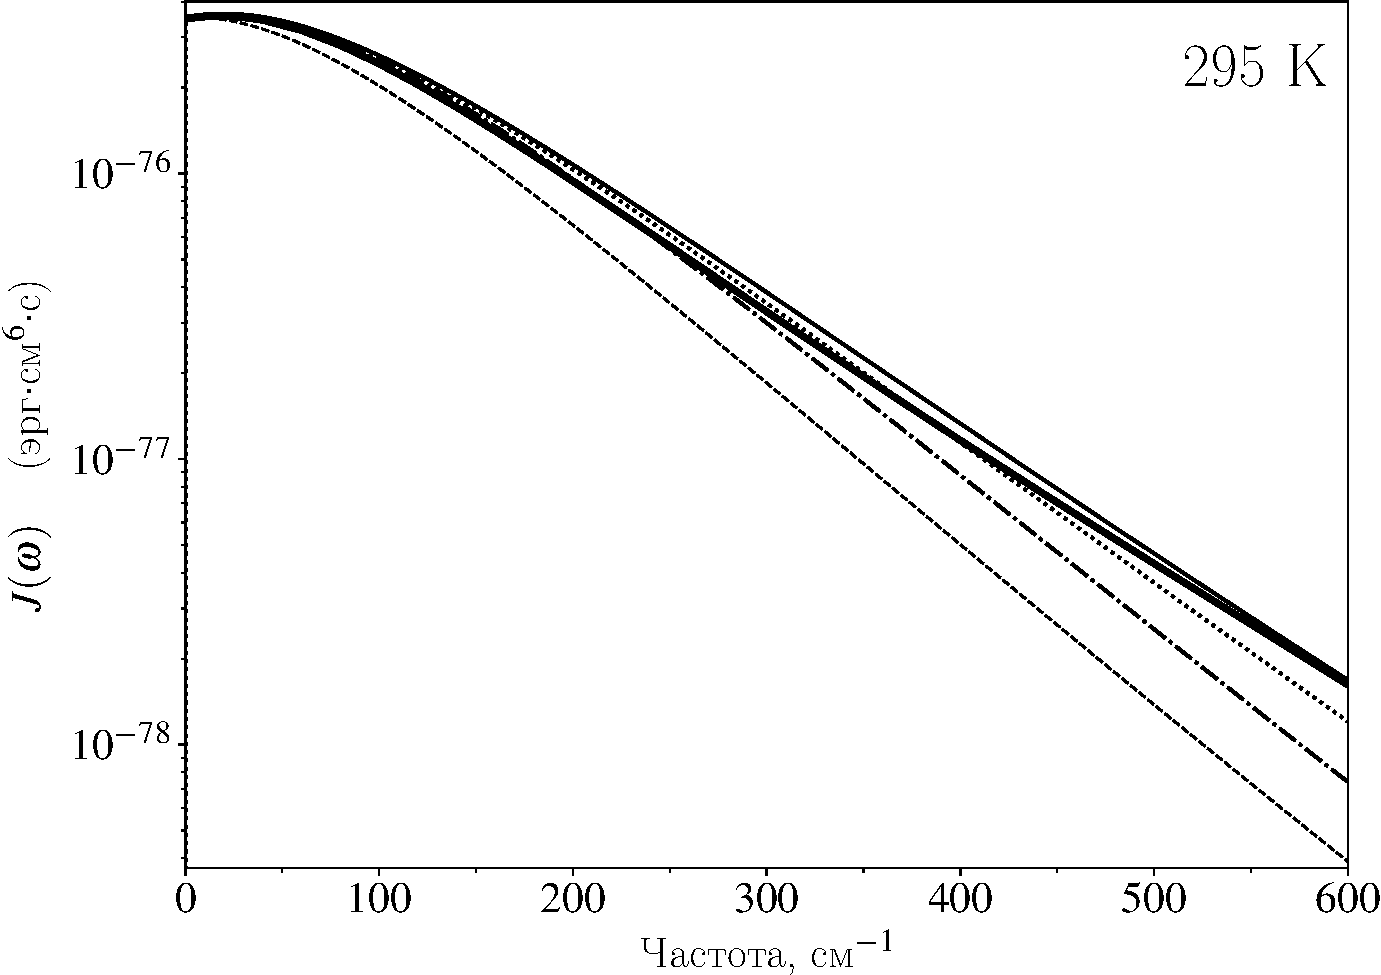
\includegraphics[width=0.7\linewidth]{./pictures/two_atom_spectra/spectral_function_desymmetrizations-crop.pdf}
    \caption{Сравнение крыльев классической, квантовой и десимметризованных спектральных функций системы He$-$Ar при температуре 295 K. Сплошной толстой линией обозначена квантовая спектральная функция \cite{buryak2014}; пунктиром -- классическая спектральная функция; пунктиром с точками -- спектральная функция, полученная в результате процедуры десимметризации D1; точечной линией -- спектральная функция, полученная в результате процедуры десимметризации D2; тонкой сплошной линией -- спектральная функция, полученная в результате процедуры десимметризации D3.}
    \label{fig:desymmetrisation-spectral-functions}
\end{figure}

Несложно убедиться, что приведенные процедуры десимметризации D1-D3 приводят к спектральным функциям, удовлетворяющим квантовому условию детального баланса. Продемонстрируем это на примере десимметризации D3, используя классическое правило детального баланса для $J_\text{class}(\omega)$:
\begin{gather}
    J_{D3}(\omega) = \exp \lb \frac{\hbar \omega}{2 \kb T} \rb J_\text{class}(\omega) \quad \implies \quad J_\text{class}(\omega) = \exp \lb -\frac{\hbar \omega}{2 \kb T} \rb J_{D3}(\omega), \label{d1} \\
    J_{D3}(-\omega) = \exp \lb -\frac{\hbar \omega}{2 \kb T} \rb J_\text{class}(-\omega) = \exp \lb -\frac{\hbar \omega}{2 \kb T} \rb J_\text{class}(\omega), \label{d2} \\
    J_{D3}(-\omega) = \exp \lb -\frac{\hbar \omega}{\kb T} \rb J_\text{D3}(\omega). \label{d3}
\end{gather}

Основываясь на рис. (\ref{fig:desymmetrisation-spectral-functions}), замечаем, что при малых частотах все спектральные функции ведут себя примерно одинаковым образом, однако с увеличением частоты различие между ними становится все больше. Одной из наиболее популярной в литературе является процедура D3. Спектральная функция, полученная в результате процедуры D3, переоценивает квантовую спектральную функцию в области крыла, однако считается, что около максимума спектра она дает наилучшую оценку. Сравнение при других температурах мы будем производить именно со спектром, полученным в результате процедуры D3. \par

\begin{figure}[H]
    \centering
    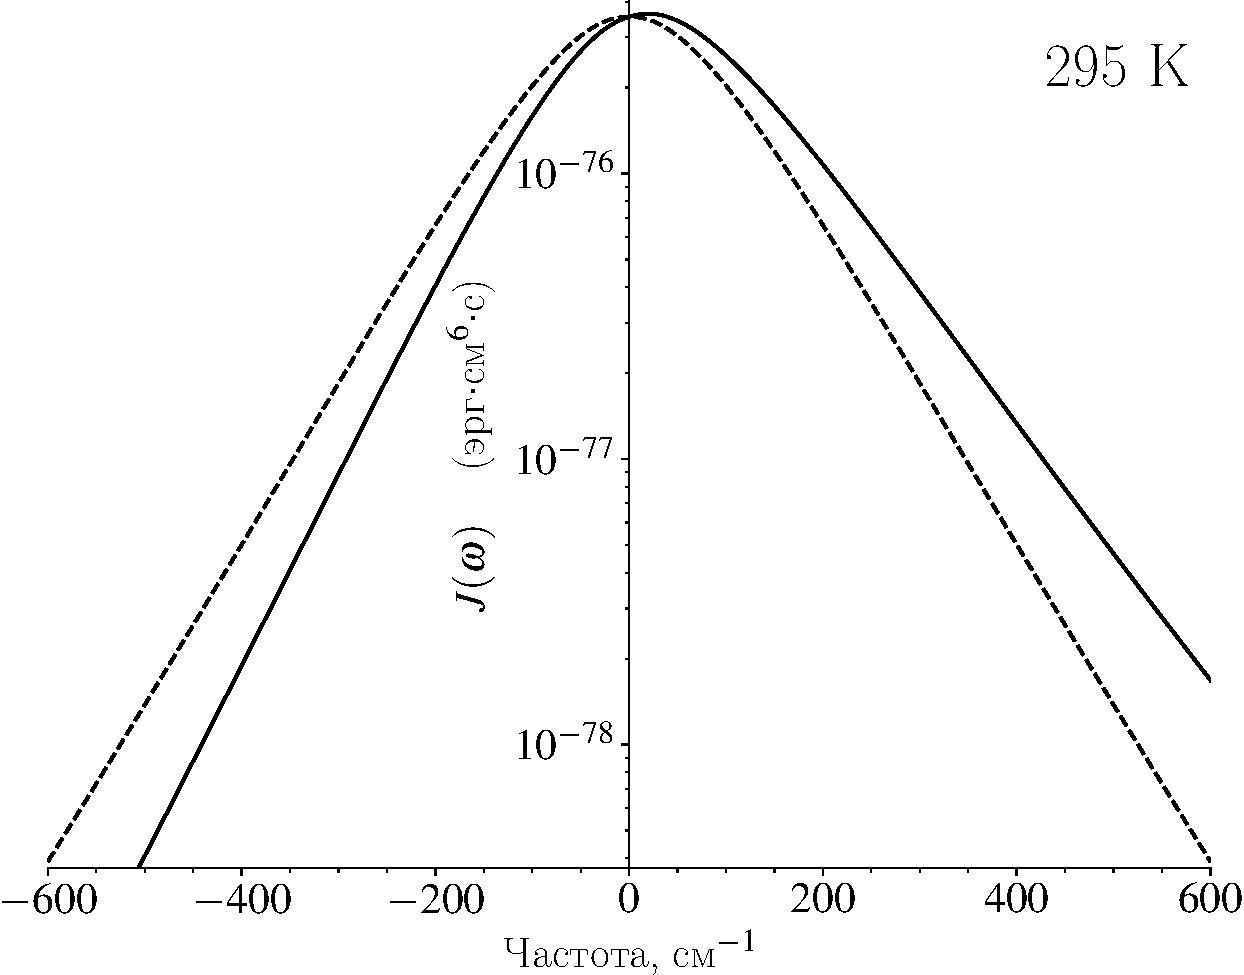
\includegraphics[width=0.49\linewidth]{./pictures/two_atom_spectra/spectral_function_d3-crop.pdf}
    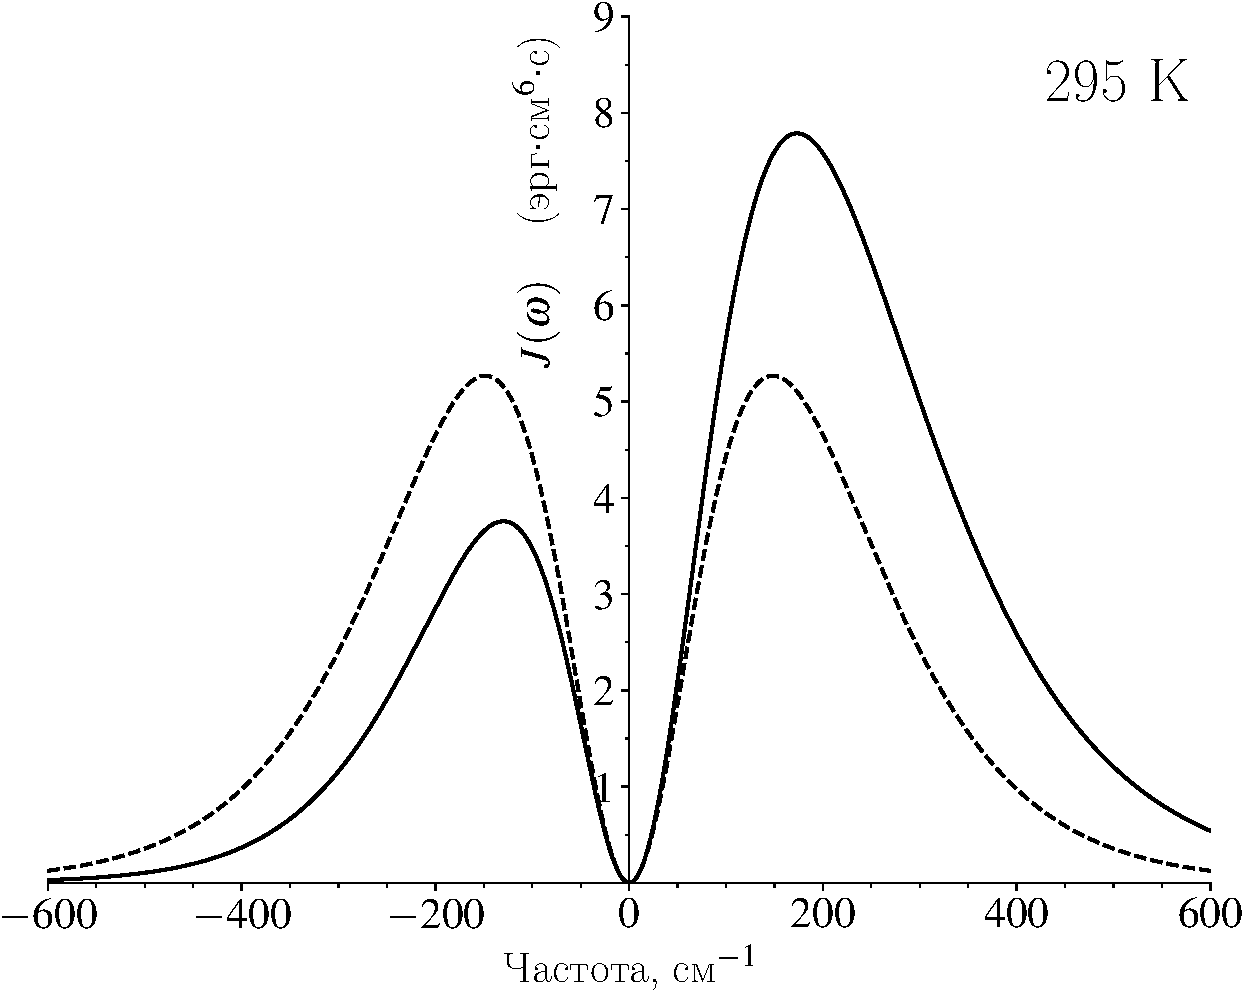
\includegraphics[width=0.49\linewidth]{./pictures/two_atom_spectra/spectrum_effect_d3-crop.pdf}
    \caption{Влияние десимметризации на спектральную функцию и спектральный профиль с учетом отрицательных частот. Пунктиром обозначены классические спектральная функция и профиль; сплошной линией -- полученные из классических в результате процедуры D3.}
    \label{fig:two-atom-d3-effect}
\end{figure}

Сравнение с экспериментальными данными на рис. (\ref{fig:two-atom-spectra}) показывает, что, несмотря на проблему выбора подходящей процедуры десимметризации, общее совпадение с экспериментальными данными оказывается неплохим. Отклонения между спектрами, полученными в результате применения различных процедур десимметризации, не превышает отклонения между квантовым профилем и экспериментальными данными. При всех температурах мы видим, что профиль, полученный в результате процедуры десимметризации D3, несколько превышает экспериментальные данные. \par 
Представленные на рис. (\ref{fig:two-atom-spectra}) спектральные профили получены в результате усреднения 2.000.000 траекторий. При всех температурах, кроме 240К, наблюдается достаточно близкое согласие с экспериментальными данными. При температуре 240К отклонение составляет порядка 10 \%, что попадает в стандартную погрешность экспериментальных данных, поэтому отклонение нельзя считать значимым. Также было обнаружено полное согласие с классическими спектрами, полученными в работе \cite{buryak2014} при помощи другой траекторной методики. 

\begin{figure}[H]
    \centering
    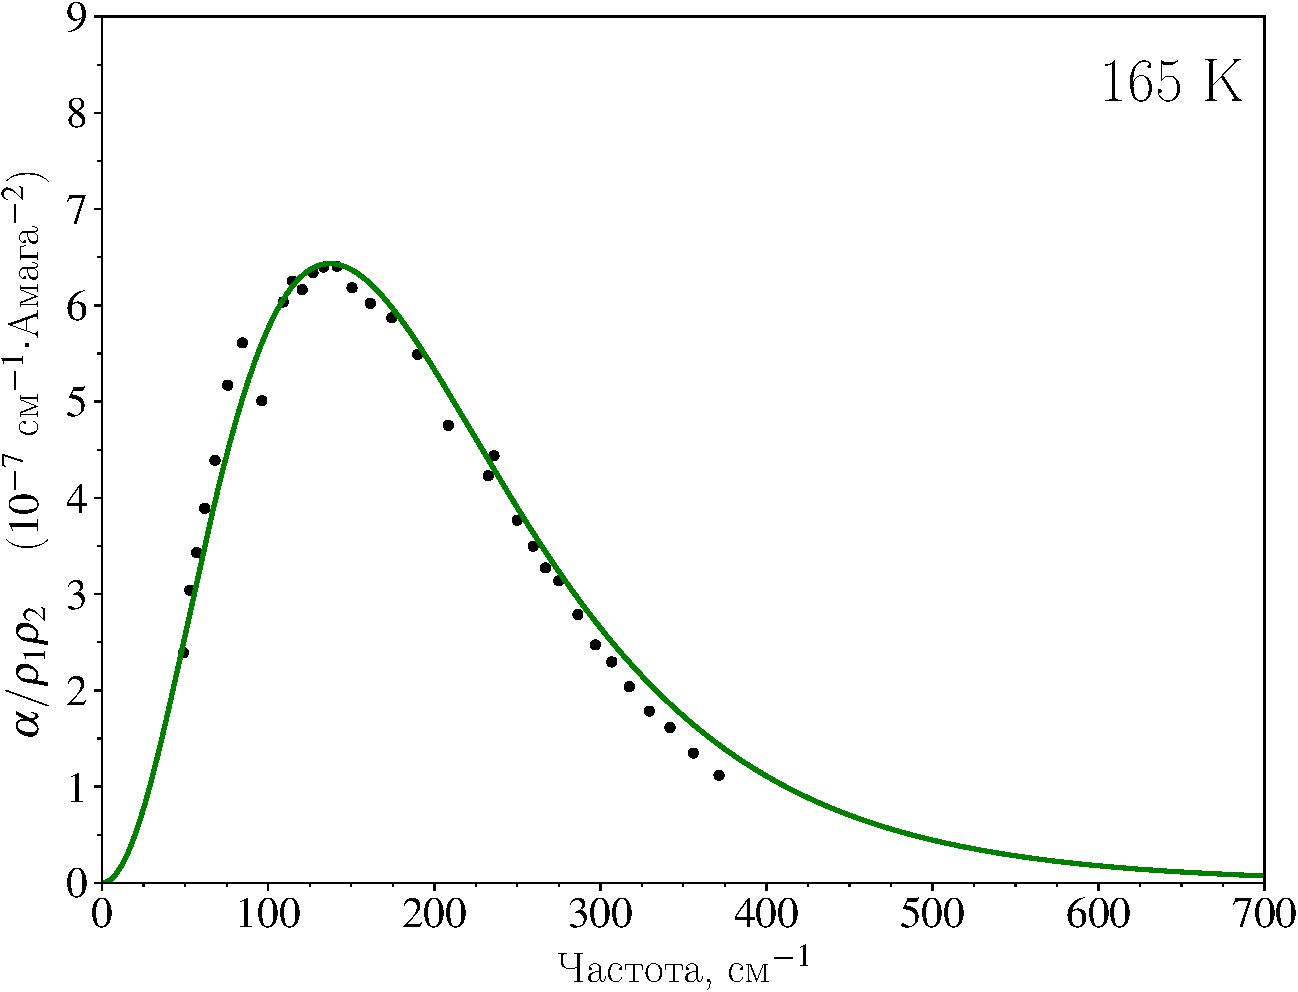
\includegraphics[width=0.49\linewidth]{./pictures/two_atom_spectra/alpha_165K-crop.pdf} 
    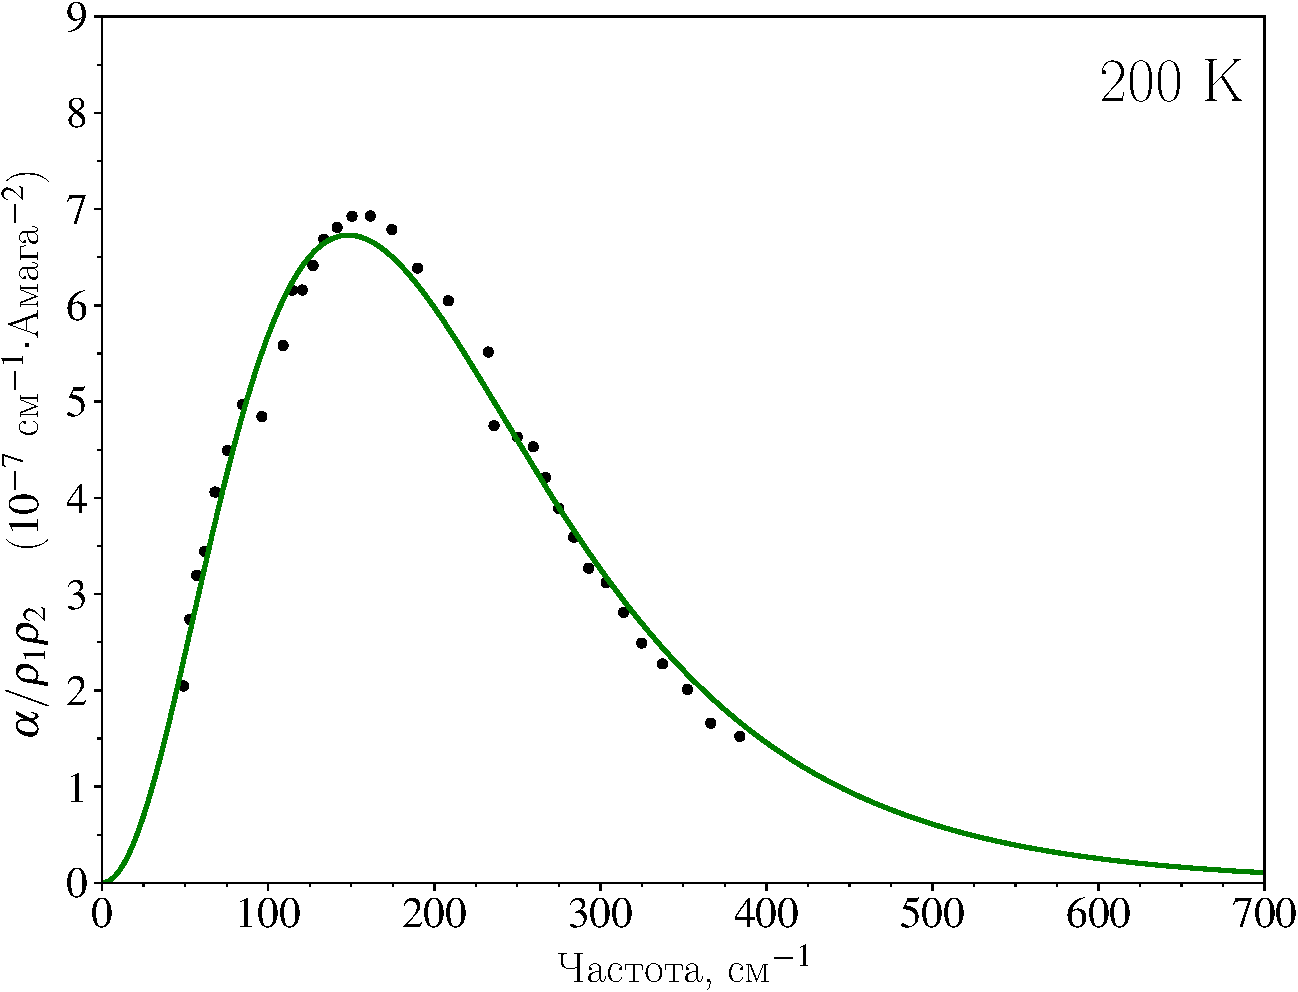
\includegraphics[width=0.49\linewidth]{./pictures/two_atom_spectra/alpha_200K-crop.pdf} \\
    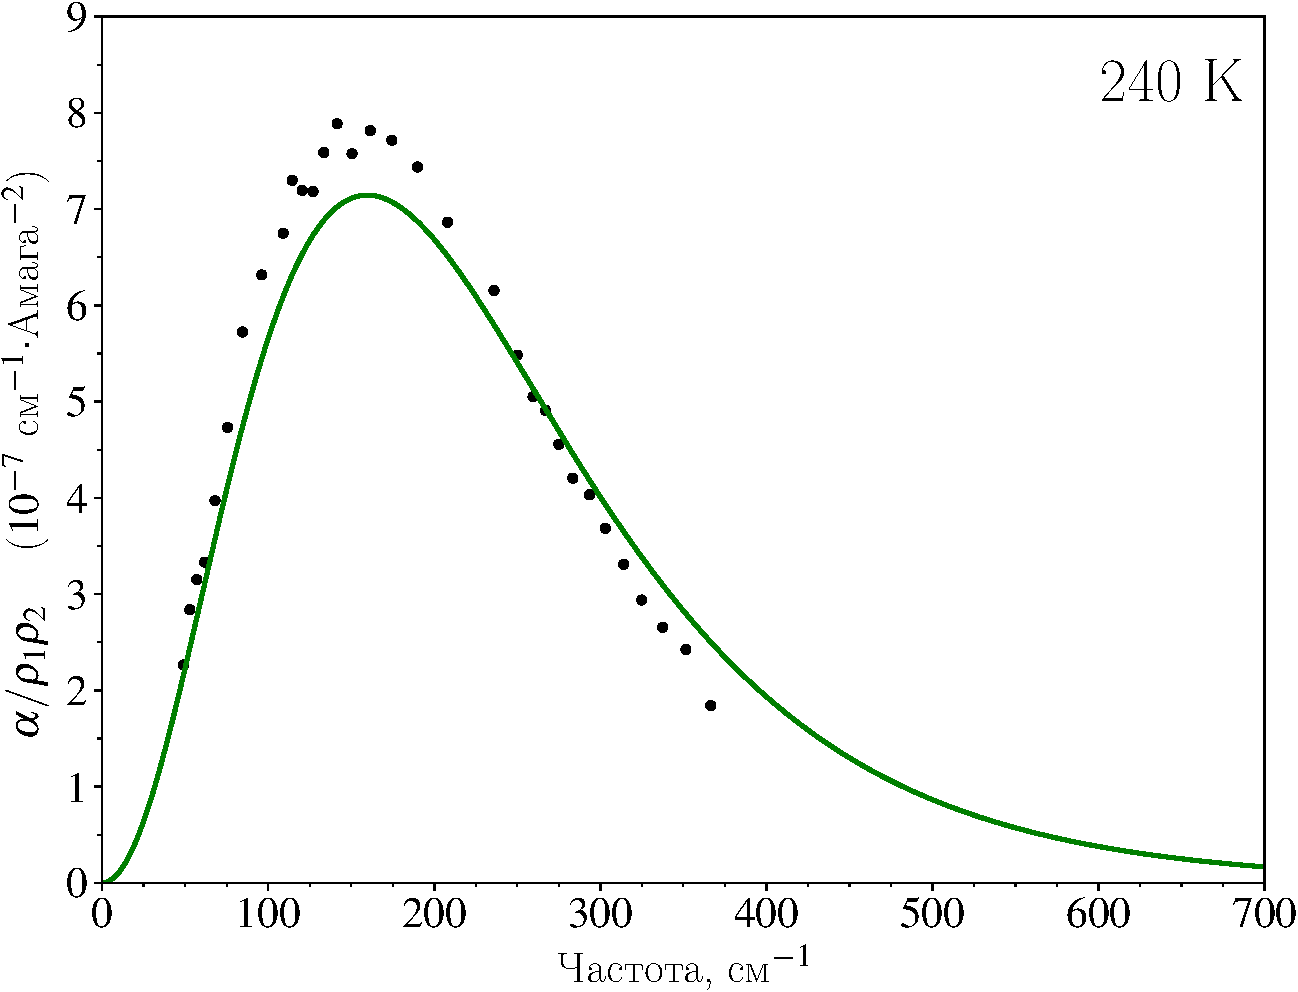
\includegraphics[width=0.49\linewidth]{./pictures/two_atom_spectra/alpha_240K-crop.pdf}
    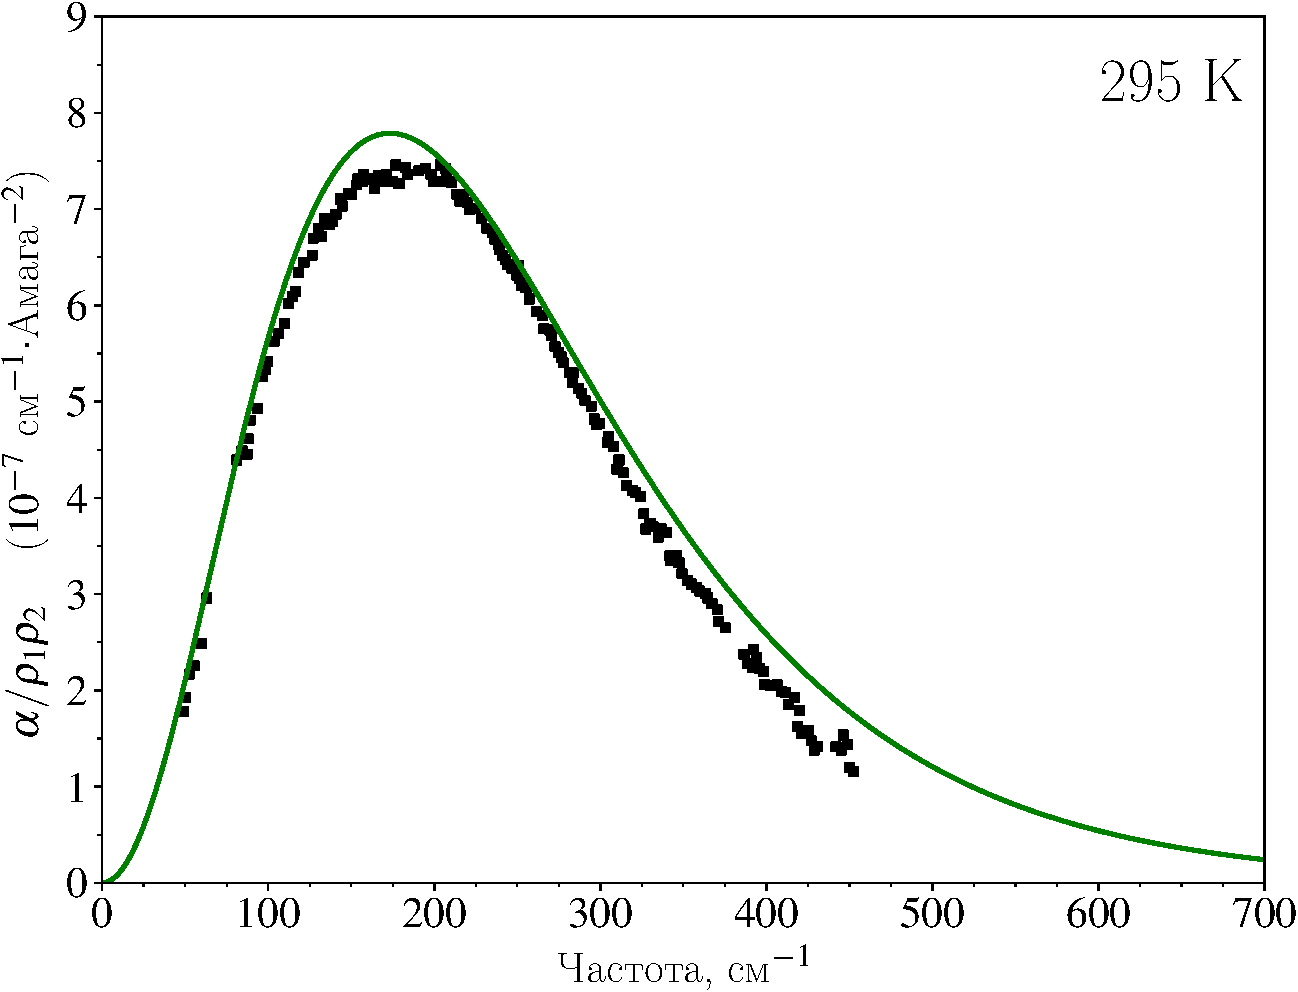
\includegraphics[width=0.49\linewidth]{./pictures/two_atom_spectra/alpha_295K-crop.pdf}
    \caption{Трансляционные спектры системы He$-$Ar при температурах 165K, 200K, 240K и 295K. Черными кружками обозначены экспериментальные данные из \cite{bukhtoyarova1977, bukhtoyarova1977_2, ryzhov1974}, квадратами -- из \cite{bosomworth1965_part2}.}
    \label{fig:two-atom-spectra}
\end{figure}

Сходимость расчета спектральной функции по Монте-Карло контролировалась при помощи спектральных моментов. Как отмечалось в теоретическом введении, спектральные моменты могут быть посчитаны как средние по фазовому пространству и как интегралы с использованием спектральной функции. Если на всех этапах траекторного расчета не допускаются систематические ошибки, то с увеличением количества траекторий моменты получаемой спектральной функции должны стремиться к моментам, полученным при усреднении по соотвествующей области фазового пространства. Так как начальные условия отбираются по области $H > 0$, то спектральные моменты для сравнения должны быть рассчитаны по соответствующей области фазового пространства. Расчет спектральных моментов производился по формулам \eqref{litreview-m0-phase-space}, \eqref{litreview-m2-phase-space}  при помощи адаптивного метода Монте-Карло \cite{hep}. В таблице (\ref{table:hear-moments}) представлены данные о сходимости спектральных профилей, представленных на рис. (\ref{fig:two-atom-spectra}). 

\begin{table}[H]
    \caption{Сравнение спектральных моментов, рассчитанных по фазовому пространству, с моментами по траекторным спектрам системы He$-$Ar}
    \begin{tabular}{c >{\centering}p{6cm} >{\centering}p{6cm} >{\centering}p{3cm}}
        \toprule
        $T$, K & Спектральные моменты $M_0$ (см$^{-1} \cdot$Амага$^{-2}$) и $M_2$ (см$^{-3} \cdot$Амага$^{-2}$) по фазовому пространству & Спектральные моменты $M_0$ (см$^{-1} \cdot$Амага$^{-2}$) и $M_2$ (см$^{-3} \cdot$Амага$^{-2}$) по траекторному спектру & Отклонение \tabularnewline
        \midrule
        \multirow{2}{*}{$165$}  & $3.113\cdot 10^{-6}$ & $3.110 \cdot 10^{-6}$ & $-0.1$ \%  \tabularnewline
                                & $3.061\cdot 10^{-2}$ & $3.077 \cdot 10^{-2}$ & $+0.5$ \%  \tabularnewline
        \midrule
        \multirow{2}{*}{$200$}  & $3.684\cdot 10^{-6}$ & $3.663 \cdot 10^{-6}$ & $-0.5$ \%  \tabularnewline
                                & $4.278\cdot 10^{-2}$ & $4.290 \cdot 10^{-2}$ & $+0.3$ \%  \tabularnewline
        \midrule
        \multirow{2}{*}{$240$}  & $4.347\cdot 10^{-6}$ & $4.337 \cdot 10^{-6}$ & $-0.2$ \%  \tabularnewline
                                & $5.912\cdot 10^{-2}$ & $5.983 \cdot 10^{-2}$ & $+1.2$ \%  \tabularnewline
        \midrule
        \multirow{2}{*}{$295$}  & $5.274\cdot 10^{-6}$ & $5.241 \cdot 10^{-6}$ & $-0.6$ \%  \tabularnewline
                                & $8.574\cdot 10^{-2}$ & $8.591 \cdot 10^{-2}$ & $+0.2$ \%  \tabularnewline
        \bottomrule
    \end{tabular}
    \label{table:hear-moments}
\end{table}



%\section{Квантовый подход к моделированию спектра}
%\section{Классический подход в лабораторной системе координат}
%\section{Вычислительные аспекты моделирования классических траекторий}

\chapter{Моделирование рототрансляционного столновительно-индуцированного спектра систем с вращательными степенями свободы}
\section{Теоретические подходы к моделированию столкновительно-индуцированных спектров}

Существующие методы расчета столкновительно-индуцированных спектров можно подразделить на квантовые и классические. Наиболее точные квантово-механические результаты можно получить с использованием close-coupling (СС) метода. В расчетах с использованием этого метода решается стационарное уравнение Шредингера в угловом базисе с полным учетом анизотропии потенциальной энергии. Этот подход требует огромных вычислительных затрат, его применение ограничено достаточно низкими температурами. В квантово-механических расчетах часто используют изотропное приближение, поскольку оно позволяет существенно уменьшить размерность базиса и сократить вычислительные затраты. В рамках этого приближения были получены отличные результаты для систем, содержащих сферически-симметричные молекулы (например, CH$_4$), и для малых линейных молекул (например, H$_2$). Подход к расчету столкновительно-индуцированных спектров в изотропном приближении долгое время развивался в примении к водородсодержащим системам, имеющим важное астрофизическое значение, таким как H$_2-$H$_2$ \cite{abel2009} и H$_2-$He \cite{abel2012}. Совпадение с экспериментальными данными считалось хорошим, по крайней мере в логарифмическом масштабе, в котором производилось сравнение, т.к. коэффициент поглощения изменяется на несколько порядков в рассматриваемом диапазоне. В работах Эль-Кадера и соавторов применяется квантовый подход с использованием эмпирических изотропных поверхностей и модельных поверхностей индуцированного дипольного момента, например, для систем CH$_4-$CH$_4$ \cite{elkader2012} и Ar$-$H$_2$ \cite{elkader2017}. \par
Квантово-механическое моделирование столкновительно-индуцированных спектров системы N$_2-$N$_2$ было впервые выполнено Борисовой и Фроммхольдом \cite{borysow1986}. В этих расчетах были использованы эффективные изотропные потенциалы и параметризованные поверхности индуцированного дипольного момента, в которых варьировались параметры, описывающие поведение дипольного момента при малых межмолекулярных расстояниях. \par
Применение изотропных поверхностей потенциальной энергии ограничено достаточно небольшой группой молекулярных систем. Обоснованность использования этого приближения может быть проверена при помощи спектральных моментов, расчет которых не требует знания динамики столкновений. Так, для системы CO$_2-$CO$_2$ на основе анализа температурных зависимостей спектральных моментов было показано, что взаимодействие молекул обладает существенной анизотропией и не может быть описано эффективным изотропным потенциалом \cite{gruszka1996}. Полное квантово-механическое рассмотрение таких систем в настоящее время не представляется возможным. В то же время большие значения моментов инерции обеих молекул позволяют с высокой степенью достоверности считать вращательное движение классическим. При достаточно высоких температурах моделирование столкновительно-индуцированных спектров может быть выполнено с использованием классического подхода. При промежуточных температурах для коррекции классических результатов применяются полуклассические процедуры десимметризации \cite{frommhold}. Классические методы подразделяются на метод молекулярной динамики \cite{gruszka1996, bussery2014} и метод классических траекторий \cite{oparin2017}. 

В работе \cite{oparin2017} был использован метод классических траекторий для расчета спектров CO$_2-$Rg, где Rg -- атом благородного газа. Уравнения движения были записаны в лабораторной системе координат, их численное решение было осуществлено при помощи специально разработанной для этой задачи процедуры типа предиктор-корректор в предположении линейной зависимости ускорения от времени. Были выделены спектральные вклады как метастабильных и свободных состояний, так и связанных состояний. Для расчета автокорреляционной функции дипольного момента, усредненной по связанным состояниям, была придумана специальная схема. \par 
В работе \cite{karman2015} был произведен расчет \textit{ab initio} поверхностей потенциальной энергии и индуцированного дипольного момента, подробно описанный в разделе \ref{section:quantum-chemistry-data}. С использованием посчитанных поверхностей производится квантово-механическое рассмотрение системы N$_2-$N$_2$ в coupled-states (CS) приближении, в котором пренебрегают внедиагональными членами оператора Кориолисова взаимодействия в гамильтониане. При одной частоте и низких энергиях авторы выполнили полный СС расчет, который показал, что CS приближение учитывает большую часть эффектов, связанных с анизотропией потенциала, и расчет коэффициента поглощения при заданном наборе частот был выполнен именно в CS приближении. В более ранней работе \cite{karman2015_h2h2} авторы предлагают эффективную методику \textit{on-the-fly} расчета матричных элементов дипольного момента, которая была использована и в расчете для N$_2-$N$_2$. Кроме переходов между свободными состояниями были учтены переходы между связанными состояниями комплекса, а также переходы из связанных состояний в свободные. Несмотря на использование CS приближения, расчет составляющей спектра, связанной с переходами между свободными состояниями, оказывается чрезвычайно тяжелым с вычислительной точки зрения и не обладает масштабируемостью для применения к системам большей размерности. \par
Молекулярно-динамическое рассмотрение системы N$_2-$N$_2$ в рототрансляционной области было проведено в работе \cite{bussery2014}. Авторы показывают, что анизотропия потенциальной энергии для системы N$_2-$N$_2$ не является ярко выраженной -- учет анизотропии увеличивает максимум спектрального профиля на $\sim 20\%$ при 149К и на $\sim 10\%$ при 296К. Авторы также производят сравнение спектральных профилей, полученных с использованием дальнодействующего дипольного момента и диполя, дополненного \textit{ab initio} расчетом при малых и средних межмолекулярных расстояниях \cite{lokshtanov2008}. Результаты показывают, что учет короткодействующей части дипольного момента приводит к увеличению максимума спектра на 10-15\%. Добавление короткодействующей части дипольного момента приводит к существенным изменениям в области крыла спектра -- интенсивность поглощения на частоте 300 см$^{-1}$ увеличивается более чем в два раза. Наилучшее совпадение теоретических спектров с экспериментальными данными было получено при температуре 149К, при более высоких температурах согласие с экспериментальными данными ухудшается, что авторы объясняют возможными систематическими ошибками в экспериментальных данных и недостаточной полнотой квантово-химических данных. Добавим, что молекулярно-динамический расчет также является очень тяжеловесным с вычислительной точки зрения.

\section{Колебательно-вращательный гамильтониан в молекулярной системе координат}

При выводе молекулярного гамильтониана для многоатомной системы часто предполагается, что амплитуда колебаний мала. Гамильтониан, полученный Вильсоном и Говардом \cite{wilson1936}, для системы с колебаниями малой амплитуды широко используется и часто служит базисом для дальнейших уточнений. Колебания большой амплитуды, проявляющиеся в слабосвязанных комплексах, не могут быть описаны при помощи того же подхода. Для описания колебаний большой амплитуды часто используются координаты Якоби, координаты Радау, гиперсферические координаты и др. \par 
Рассмотрим систему из $N$ частиц с массами $\lb m_1, \dots m_N \rb$ и координатами $\lb \mf{r}_1, \dots, \mf{r}_N \rb$ в лабораторной системе координат. Лагранжева кинетическая энергия в лабораторной системе координат записывается как
\begin{gather}
    T_\text{tot} = \frac{1}{2} \sum_{k = 1}^N m_k \dot{\mf{r}}_k^2.
\end{gather}

Чтобы отделить трансляционные степени свободы, введем координаты Якоби \cite{greiner, littlejohn1995}, являющиеся обобщением координат, используемых в двухатомных системах. Переход к трансляционно-инвариантному набору координат может быть осуществлен следующим образом \cite{greiner}
\begin{gather}  
    \begin{aligned}
        \bs{\rho}_1 &= \frac{m_1 \mf{r}_1}{m_1} - \mf{r}_2 = \mf{r}_1 - \mf{r}_2, \\
        \bs{\rho}_2 &= \frac{m_1 \mf{r}_1 + m_2 \mf{r}_2}{m_1 + m_2}, \\
        \bs{\rho}_j &= \frac{\displaystyle \sum_{k = 1}^j m_k \mf{r}_k}{\displaystyle \sum_{k = 1}^j m_k} - \mf{r}_{j + 1}, \quad 2 < j < N \\
        \bs{\rho}_N &= \frac{1}{M} \sum_{k = 1}^N m_k \mf{r}_k,
    \end{aligned}
\end{gather}
%
где через $M$ обозначена суммарная масса системы частиц. \par
Первый вектор Якоби $\bs{\rho}_1$ соединяет частицы 1 и 2. Второй вектор Якоби соединяет центр масс первых двух частиц и третью частицу. Третий вектор Якоби соединяет центр масс первых трех частиц и четвертую частицу и т.д. Последний вектор Якоби направлен в центр масс системы. Пример векторов Якоби для системы, соcтоящей из трех частиц, приведен на рис. (\ref{fig:jacobi_coordinates}). 

\begin{figure}
    \centering
    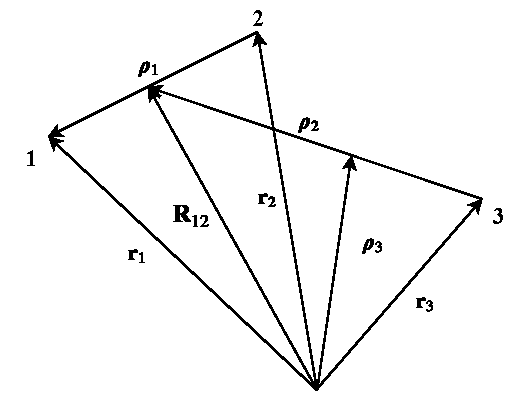
\includegraphics[width=0.5\linewidth]{pictures/jacobi_coordinates.pdf}
    \caption{Координаты Якоби  для системы из 3 частиц, пронумерованных 1, 2, 3. Через $\mf{R}_{12}$ обозначен вектор, направленный в центр масс пары частиц 1 и 2.}
    \label{fig:jacobi_coordinates}
\end{figure}

Можно показать, что кинетическая энергия в лагранжевой форме, выраженная через векторы Якоби, записывается как \cite{greiner} 
\begin{gather}
    T_\text{tot} = \frac{1}{2} M \dot{\bs{\rho}}_N^2 + \frac{1}{2} \sum_{k = 1}^{N - 1} \mu_k \dot{\bs{\rho}}_k^2,
\end{gather}
%
где приведенные массы $\mu_j$ связаны с исходными массами $m_j$ следующими соотношениями
\begin{gather}
    \frac{1}{\mu_j} = \frac{1}{M_j} + \frac{1}{m_{j+1}}, \quad M_j = \sum_{k = 1}^j m_k, \quad j = 1 \dots N - 1. \label{polyatom-jacobi-masses}
\end{gather}

Данная последовательность введения векторов Якоби не является единственно возможной. Выбор векторов Якоби в каждом отдельном случае обусловлен структурой рассматриваемой системы. Описанная последовательность является общим случаем, в котором получена кинетическая энергия для системы из $N$ частиц. При другом выборе векторов Якоби общая форма кинетической энергии сохранится, однако изменятся приведенные массы $\mu_j$. \par
Отделяя центр масс, мы приходим к следующей форме кинетической энергии
\begin{gather}
    \Tl = \frac{1}{2} \sum_{k = 1}^{N - 1} \mu_k \dot{\bs{\rho}}_k^2.
\end{gather}

Для отделения вращательных степеней свободы введем подвижную систему координат. Лабораторная и подвижная системы координат связаны друг с другом матрицей ортогонального преобразования $\bbS$ \cite{goldstein}. Обозначим через $\mf{R}_j$ координаты векторов Якоби в подвижной системе координат. Введенные векторы $\mf{R}_j$ связаны с векторами в лабораторной системе линейным преобразованием
\begin{gather}
    \mf{R}_j = \bbS \boldsymbol{\rho}_j.
\end{gather}
Будем рассматривать параметризацию матрицы ортогонального преобразования $\bbS$ тройкой углов Эйлера $\Phi$, $\Theta$, $\Psi$ \cite{goldstein}
\begin{gather}
    \bbS = 
    \begin{bmatrix}
        \cos \Psi \cos \Phi - \cos \Theta \sin \Phi \sin \Psi & -\sin \Psi \cos \Phi - \cos \Theta \sin \Phi \cos \Psi & \sin \Theta \sin \Phi \\ 
        \cos \Psi \sin \Phi + \cos \Theta \cos \Phi \sin \Psi & -\sin \Psi \sin \Phi + \cos \Theta \cos \Phi \cos \Psi & - \sin \Theta \cos \Phi \\
        \sin \Theta \sin \Psi & \sin \Theta \cos \Psi & \cos \Theta
    \end{bmatrix}.
\end{gather}

Лагранжева кинетическая энергия в подвижной системе отсчета может быть записана как \cite{sutcliffe}
\begin{gather}
    \Tl = \frac{1}{2} \sum_{i = 1}^{N-1} \mu_i \dot{\mf{R}}_i^2 + \frac{1}{2} \sum_{i = 1}^{N - 1} \mu_i \lsq \boldsymbol{\Omega} \times \mf{R}_i \rsq^2 + \boldsymbol{\Omega}^{+} \sum_{i = 1}^{N - 1} \mu_i \lsq \mf{R}_i \times \dot{\mf{R}}_i \rsq,
\end{gather}
%
где $\boldsymbol{\Omega}$ -- вектор угловой скорости в проекции на подвижную систему координат. Вектор угловой скорости $\boldsymbol{\Omega}$ связан с углами Эйлера и эйлеровыми скоростями следующим соотношением
\begin{gather}
    \boldsymbol{\Omega} = \bbV \dot{\boldsymbol{\Upsilon}}_e = 
    \begin{bmatrix}
        \sin \Theta \sin \Psi & \cos \Psi & 0 \\
        \sin \Theta \cos \Psi & -\sin \Psi & 0 \\
        \cos \Theta & 0 & 1 
    \end{bmatrix}
    \begin{bmatrix}
        \dot{\Phi} \\ \dot{\Theta} \\ \dot{\Psi}
    \end{bmatrix}. \label{polyatom-matrixV}
\end{gather}

Введем набор внутренних координат $\mf{q} = \lb q_1, \dots q_s \rb$ и, используя связь координат Якоби с введенными координатами $\mf{R}_j = \mf{R}_j(\mf{q})$, перепишем выражение для кинетической энергии в форме \cite{petrov2015}
\begin{gather}
    \Tl = \frac{1}{2} \dot{\mf{q}}^+ \bba \dot{\mf{q}} + \bOmega^+ \bbA \mf{q} + \frac{1}{2} \bOmega^+ \bbI \, \bOmega, \label{body-fixed-lagrange-energy} 
\end{gather}
%
где через $\bba, \bbA, \bbI$ обозначены матрица относительной кинетической энергии, кориолисова матрица и матрица тензора инерции, соответственно. Элементы матриц относительной кинетической энергии и кориолисова взаимодействия заданы следующими выражениями
\begin{gather}
    \bba_{jk} = \sum_{i = 1}^{N - 1} \mu_i \frac{\partial \mf{R}_i}{\partial q_j} \frac{\partial \mf{R}_i}{\partial q_k}, \quad \bbA_{jk} = \sum_{i = 1}^{N - 1} \mu_i \lsq \mf{R}_i \times \frac{\partial \mf{R}_i}{\partial q_k} \rsq_j. \label{polyatom-kinetic-energy-matrices}
\end{gather}

С целью перехода к гамильтоновой форме выражение для кинетической энергии \eqref{body-fixed-lagrange-energy} удобно переписать в матричном виде
\begin{gather}
    \Tl = \frac{1}{2} \begin{bmatrix} \bOmega^+ & \dot{\mf{q}}^+ \end{bmatrix} \bbB \begin{bmatrix} \bOmega \\ \dot{\mf{q}} \end{bmatrix}, \label{polyatom-block-matrix-kin-energy}
\end{gather}
%
где через $\bbB$ обозначена блочная матрица со следующими элементами 
\begin{gather}
    \bbB = \begin{bmatrix} 
    \bbI & \bbA \\ \bbA^+ & \bba 
    \end{bmatrix}.
\end{gather}

Можно показать, что если ввести величину $\mf{J}$ как производную кинетической энергии в лагранжевой форме $\Tl$ по вектору угловой скорости $\bOmega$, то $\mf{J}$ есть вектор углового момента в подвижной системе координат (Приложение 4.А). Обобщенные импульсы $\mf{p}$, сопряженные координатам $\mf{q}$, по определению равны производным кинетической энергии в лагранжевой форме $\Tl$ по обобщенным скоростям $\dot{\mf{q}}$: 
\begin{gather}
    \mf{J} = \frac{\partial \Tl}{\partial \bOmega} = \bbI \bOmega + \bbA \dot{\mf{q}}, \label{polyatom-angmom1} \\
\mf{p} = \frac{\partial \Tl}{\partial \dot{\mf{q}}} = \bbA^+ \bOmega + \bba \dot{\mf{q}} \label{polyatom-gen-momenta}.
\end{gather}

Заметим, что выражения \eqref{polyatom-angmom1}, \eqref{polyatom-gen-momenta} могли быть получены дифференцированием выражения  \eqref{polyatom-block-matrix-kin-energy} по блочному вектору с компонентами $\bOmega$ и $\dot{\mf{q}}$. Выражения для углового момента и обобщенных импульсов объединим в один блочный вектор
\begin{gather}
    \begin{bmatrix} \mf{J} \\ \mf{p} \end{bmatrix} = \bbB \begin{bmatrix} \bOmega \\ \dot{\mf{q}} \end{bmatrix} = 
    \begin{bmatrix} \bbI & \bbA \\ \bbA^+ & \bba \end{bmatrix} \begin{bmatrix} \bOmega \\ \dot{\mf{q}} \end{bmatrix}.
\end{gather}

Для того чтобы выразить лагранжевы переменные из полученного выражения, нам необходимо обратить блочную матрицу $\bbB$. Это обращение удобно выполнить при помощи формул Фробениуса \cite{gantmaher}. Через $\bbG$ обозначают обратную матрицу к $\bbB$, ее матричные компоненты выражаются как \cite{petrov2015}
\begin{gather}
    \begin{aligned}
        \bbG_{11} &= \lb \bbI - \bbA \bba^{-1} \bbA^+ \rb^{-1}, \\
        \bbG_{12} &= -\bbI^{-1} \bbA \bbG_{22} = -\bbG_{11} \bbA \bba^{-1}, \\
        \bbG_{21} &= -\bba^{-1} \bbA^+ \bbG_{11} = \bbG_{22} \bbA^+ \bbI^{-1}, \\
        \bbG_{22} &= \lb \bba - \bbA^+ \bbI^{-1} \bbA \rb^{-1}.
    \end{aligned} \label{polyatom-frobenius}
\end{gather}

Переход от кинетической энергии в форме Лагранжа к кинетической энергии в форме Гамильтона осуществляем при помощи стандартной процедуры \cite{goldstein}
\begin{gather}
    \Th = \begin{bmatrix} \bOmega^+ & \dot{\mf{q}}^+ \end{bmatrix} \begin{bmatrix} \mf{J} \\ \mf{p} \end{bmatrix} - \Tl = \frac{1}{2} \begin{bmatrix} \mf{J}^+ & \mf{p}^+ \end{bmatrix} \bbG \begin{bmatrix} \mf{J} \\ \mf{p} \end{bmatrix} = \frac{1}{2} \mf{J}^+ \bbG_{11} \mf{J} + \mf{J}^+ \bbG_{12} \mf{p} + \frac{1}{2} \mf{p}^+ \bbG_{22} \mf{p}, \label{general-rovibrational-kin-energy} 
\end{gather}
а полный колебательно-вращательный гамильтониан получается в результате добавления потенциальной энергии к $\Th$
\begin{gather}
    H = \frac{1}{2} \mf{J}^+ \bbG_{11} \mf{J} + \mf{J}^+ \bbG_{12} \mf{p} + \frac{1}{2} \mf{p}^+ \bbG_{22} \mf{p} + U(\mf{q}). \label{general-rovibrational-hamiltonian} 
\end{gather}

В данной работе мы будем рассматривать системы, состоящие из жесткой линейной молекулы и атома или из двух жестких линейных молекул. \par
В случае системы атом$-$линейная молекула построим вектор Якоби вдоль линейной молекулы, тогда второй вектор Якоби соединяет центр масс линейной молекулы с атомом. Определим подвижную систему координат таким образом, чтобы построенные вектора Якоби $\mf{R}_1$, $\mf{R}_2$ задавали плоскость $OXZ$ подвижной системы. Дополнительно потребуем, чтобы вектор $\mf{R}_2$, соединяющий центр масс линейной молекулы с атомом, лежал вдоль оси $OZ$ (см. рис. \ref{fig:body-fixed-linear-atom}). Такое определение системы координат известно как $R$-вложение \cite{tennyson1986}. Обозначим длину линейной молекулы через $l$.
    
\begin{figure}[H]
    \centering
    %\begin{minipage}{0.49\linewidth}
    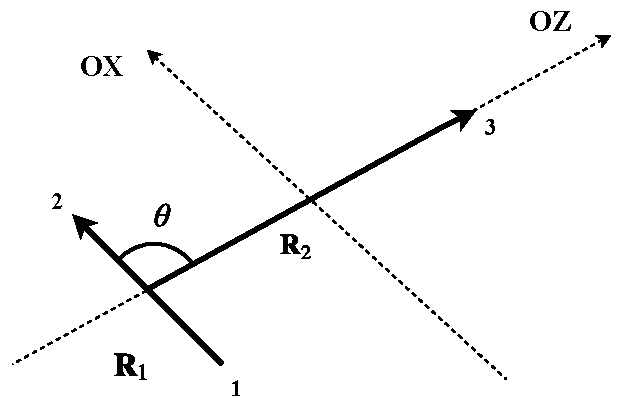
\includegraphics[width=0.5\linewidth]{pictures/triatom_coordinates.pdf}
    %\end{minipage}
    %\begin{minipage}{0.49\linewidth}
    %    Взять картинку из будущей статьи с N$_2$-N$_2$
    %\end{minipage}
    \caption{Молекулярно-фиксированная система координат для системы линейная молекула-атом}
    \label{fig:body-fixed-linear-atom}
\end{figure}

В качестве обобщенных координат выберем $R$ -- длину вектора Якоби $\mf{R}_2$, или, что эквивалентно, расстояние от атома до центра масс линейной молекулы, и угол $\theta$ между векторами Якоби $\mf{R}_1$ и $\mf{R}_2$. Угол $\theta$ отсчитывается от оси $OZ$ в сторону положительного направления оси $OX$, его область значений -- от $0$ до $\pi$. Выпишем координаты векторов в подвижной системе через обобщенные координаты $\mf{q} = \lb R, \theta \rb$: 
\begin{gather}
    \begin{aligned}
        X_1 &= l \sin \theta \\
        Y_1 &= 0 \\
        Z_1 &= l \cos \theta
    \end{aligned} \qquad
    \begin{aligned}
        X_2 &= 0 \\ 
        Y_2 &= 0 \\
        Z_2 &= R 
    \end{aligned}. \label{linear-molecule-atom-jacobi-coords}
\end{gather}

Вывод дальнейших выражений реализовывался в системе компьютерной алгебры Maple. Координаты векторов Якоби \eqref{linear-molecule-atom-jacobi-coords} использовались для расчета компонент матриц относительной кинетической энергии, кориолисова взаимодействия и тензора инерции по выражениям \eqref{polyatom-kinetic-energy-matrices}. В случае системы атом$-$линейная молекула блоки матрицы $\bbG$ могут быть получены в компактном виде. Уже для случая двух жестких линейных молекул выражения для блоков матрицы $\bbG$ оказываются слишком громоздкими, поэтому была разработана схема реализации траекторного расчета, избегающая аналитической работы с компонентами этих матриц, переносимая на системы с произвольным количеством вращательных степеней свободы. \par
В качестве примера системы атом$-$линейная молекула мы выбрали CO$_2-$Ar. Внутримолекулярные колебания молекулы CO$_2$ происходят существенно быстрее межмолекулярных движений комплекса с атомом аргона, поэтому мы предполагаем, что можно пренебречь взаимодействием колебательных мод, и в дальнейшем рассмотрении считаем молекулу CO$_2$ жесткой. 
Приведенные массы частиц Якоби согласно \eqref{polyatom-jacobi-masses} равны
\begin{gather}
    \mu_1 = \frac{m_1}{2}, \quad \mu_2 = \frac{m_2 \lb 2 m_1 + m_3 \rb}{2 m_1 + m_2 + m_3},
\end{gather}
% 
где через $m_1$ обозначена масса атома кислорода, через $m_2$ -- масса атома аргона, через $m_3$ -- масса атома углерода. \par
При помощи системы компьютерной алгебры были получены следующие выражения для матриц кинетической энергии в форме Лагранжа
\begin{gather}
	\bba =
	\begin{bmatrix}
		\mu_2 & 0 \\
		0 & \mu_1 l^2
	\end{bmatrix}, \quad 
	\bbA = 
	\begin{bmatrix}
		0 & 0 \\
		0 & \mu_1 l^2 \\
		0 & 0 
	\end{bmatrix}, \quad
	\bbI = 
	\begin{bmatrix}
		\mu_1 l^2 \cos^2 \theta + \mu_2 R^2 & 0 & -\mu_1 l^2 \sin \theta \cos \theta \\
		0 & \mu_1 l^2 + \mu_2 R^2 & 0 \\
		- \mu_1 l^2 \sin \theta \cos \theta & 0 & \mu_1 l^2 \sin^2 \theta
	\end{bmatrix}. \notag
\end{gather}

Подставив полученные выражения для матриц в формулы Фробениуса \eqref{polyatom-frobenius}, приходим к следующим выражениям для матриц, определяющим кинетическую энергию в форме Гамильтона 
\begin{gather}
	\bbG_{11} =
	\begin{bmatrix}
		\dfrac{1}{\mu_2 R^2} & 0 & \dfrac{\ctg \theta}{\mu_2 R^2} \\
		0 & \dfrac{1}{\mu_2 R^2} & 0 \\
		\dfrac{\ctg \theta}{\mu_2 R^2} & 0 & \dfrac{\ctg^2 \theta}{\mu_2 R^2} + \dfrac{1}{\mu_1 l^2 \sin^2 \theta}
	\end{bmatrix}, \quad
	\bbG_{12} =
	\begin{bmatrix}
		0 & 0 \\
		0 & - \dfrac{1}{\mu_2 R^2} \\
		0 & 0
	\end{bmatrix}, \quad 
	\bbG_{22} = 
	\begin{bmatrix}
		\dfrac{1}{\mu_2} & 0 \\
		0 & \dfrac{1}{\mu_2 R^2} + \dfrac{1}{\mu_1 l^2}
	\end{bmatrix}. \notag
\end{gather}

Итак, кинетическая энергия в форме Гамильтона для системы CO$_2-$Ar в выбранной нами молекулярной системе отсчета получается следующей
\begin{gather}
\Th = \frac{1}{2 \mu_2} p_R^2 + \lb \frac{1}{2 \mu_2 R^2} + \frac{1}{2 \mu_1 l^2} \rb p_\theta^2 - \frac{1}{\mu_2 R^2} p_\theta \Jy + \frac{1}{2 \mu_2 R^2} \Jy^2 + \frac{1}{2 \mu_2 R^2} \Jx^2 + \frac{1}{2 \sin^2 \theta} \lb \frac{\cos^2 \theta}{\mu_2 R^2} + \frac{1}{\mu_1 l^2} \rb \Jz^2 + \notag \\
+ \frac{\ctg \theta}{\mu_2 R^2} \Jx \Jz. 
\end{gather}

В случае системы, состоящей из двух жестких линейных молекул, удобно построить векторы Якоби вдоль каждой из линейных молекул, тогда третий вектор соединяет их центры масс. Определим подвижную систему координат таким образом, чтобы вектор, соединяющий центры масс линейных молекул, лежал на оси $OZ$ подвижной системы. Потребуем, чтобы вектор, определяющий одну из линейных молекул, лежал в плоскости $OXZ$ подвижной системы (рис. \ref{fig:two-linear-molecules-body-fixed}). Вторая молекула при этом может выходить из плоскости подвижной системы; для того чтобы описать ее ориентацию, необходимо ввести два угла, тогда как для описания ориентации первой молекулы достаточно одного полярного угла. Введя таким образом систему координат, мы заведомо сделали линейные молекулы неравноправными, так что соответствующие им координаты будут входить в кинетическую энергию неодинаковым образом. Обозначим длины линейных молекул через $l_1$ и $l_2$, соответственно. В качестве обобщенных координат выберем $R$ -- расстояние между центрами масс линейных молекул, $\theta_1$, $\theta_2$ -- полярные углы линейных молекул в плоскости $OXZ$, отсчитываемые от оси $OZ$ в сторону положительного направления оси $OX$, $\varphi$ -- угол между плоскостью $OXZ$ и плоскостью, заданной молекулой, не лежащей в плоскости $OXZ$, и центром масс другой молекулы. Обобщенные координаты объединим в вектор $\mf{q} = \lb R, \varphi, \theta_1, \theta_2 \rb$. 

\begin{figure}[H]
    \centering
    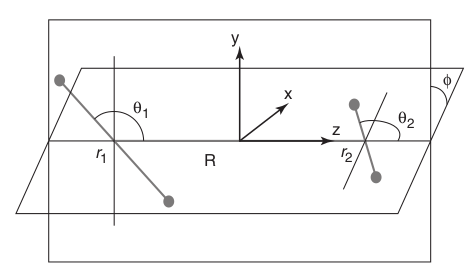
\includegraphics[width=0.5\linewidth]{pictures/n2n2_coordinate_frame.png}
    \caption{Молекулярно-фиксированная система координат для системы из двух линейных молекул}
    \label{fig:two-linear-molecules-body-fixed}
\end{figure}

Выпишем координаты векторов Якоби в подвижной системе через обобщенные координаты 
\begin{gather}
    \begin{aligned}
        X_1 &= l_1 \sin \theta_1 \\
        Y_1 &= 0 \\
        Z_1 &= l_1 \cos \theta_1 
    \end{aligned} \qquad
    \begin{aligned}
        X_2 &= l_2 \cos \varphi \sin \theta_2 \\
        Y_2 &= l_2 \sin \varphi \sin \theta_2 \\
        Z_2 &= l_2 \cos \theta_2
    \end{aligned} \qquad
    \begin{aligned}
        X_3 &= 0 \\
        Y_3 &= 0 \\
        Z_3 &= R
    \end{aligned} \label{polyatom-linear-linear-coordinates}
\end{gather}

В качестве примера системы, состоящей из двух линейных молекул, выбрана N$_2-$N$_2$. Приведенные массы частиц Якоби равны
\begin{gather}
    \mu_1 = \frac{m}{2}, \quad \mu_2 = \frac{m}{2}, \quad \mu_3 = 2m, \label{polyatom-n2n2-jacobi-masses}
\end{gather}
%
где через $m$ обозначена масса атома азота. Длины линейных молекул в дальнейшем обозначаются одинаково $l = l_1 = l_2$.

Выражения для матриц кинетической энергии в форме Лагранжа были получены из \eqref{polyatom-linear-linear-coordinates} при помощи системы компьютерной алгебры. Введенный набор координат является ортогональным, т.к. матрица относительной кинетической энергии оказывается диагональной. Приводим выражения для случая двух произвольных линейных молекул через массы частиц Якоби; выражения для конкретного случая N$_2-$N$_2$ получаются в результате подстановки масc \eqref{polyatom-n2n2-jacobi-masses}.  
\begin{gather}
\bba = 
\begin{bmatrix}
\mu_3 & 0 & 0 & 0 \\
0 & \mu_2 l_2^2 \sin^2 \theta_2 & 0 & 0 \\
0 & 0 & \mu_1 l_1^2 & 0 \\
0 & 0 & 0 & \mu_2 l_2^2 \\ 
\end{bmatrix}, \quad  
\bbA = 
\begin{bmatrix}
0 & -\mu_2 l_2^2 \cos \varphi \sin \theta_2 \cos \theta_2 & 0 & -\mu_2 l_2^2 \sin \varphi  \\
0 & -\mu_2 l_2^2 \sin \varphi \sin \theta_2 \cos \theta_2 & \mu_1 l_1^2 & \mu_2 l_2^2 \cos \varphi \\
0 &  \mu_2 l_2^2 \sin^2 \theta_2 & 0 & 0
\end{bmatrix} \notag 
\end{gather}

Компоненты матрицы тензора инерции в подвижной системе отсчета получаются следующие
\begin{gather}
    \begin{aligned}
        I_{XX} &= \mu_1 l_1^2 \cos^2 \theta_1 + \mu_2 l_2^2 (\sin^2 \varphi \sin^2 \theta_2 + \cos^2 \theta_2) + \mu_3 R^2, \\ 
        I_{XY} &= -\mu_2 l_2^2 \sin \varphi \cos \varphi \sin^2 \theta_2, \\ 
        I_{XZ} &= -\mu_1 l_1^2 \sin \theta_1 \cos \theta_1 - \mu_2 l_2^2 \cos \varphi \sin \theta_2 \cos \theta_2, \\
        I_{YY} &= \mu_1 l_1^2 + \mu_2 l_2^2 (\cos^2 \varphi \sin^2 \theta_2 + \cos^2 \theta_2) + \mu_3 R^2, \\
        I_{YZ} &= -\mu_2 l_2^2 \sin \varphi \sin \theta_2 \cos \theta_2, \\
        I_{ZZ} &= \mu_1 l_1^2 \sin^2 \theta_1 + \mu_2 l_2^2 \sin^2 \theta_2.  
    \end{aligned} 
\end{gather}

Как уже было сказано, выражения для блоков матрицы $\bbG$ в этом случае получаются слишком громоздкими для работы, поэтому не приводятся. Для реализации траекторного расчета нет необходимости получать аналитические выражения для этих матриц. 

\section{Описание молекулярного вращения в подвижной системе координат} \label{section:rotational-dynamics}

В отсутствии внешних сил угловой момент $\mf{j}$ в лабораторной системе координат является векторным интегралом движения. Компоненты вектора углового момента в подвижной системе отсчета связаны с компонентами в лабораторной системе матрицей $\bbS$
\begin{gather}
    \mf{J} = \bbS \mf{j}. \label{polyatom-j-connection}
\end{gather}

Производная вектора углового момента в подвижной системе удовлетворяет следующему соотношению \cite{goldstein}
\begin{gather}
    \dot{\mf{J}} + \lsq \bOmega \times \mf{J} \rsq = 0.
\end{gather}

Используя теорему Донкина, можно показать \cite{petrov2015}, что 
\begin{gather}
    \bOmega = \frac{\partial \Th}{\partial \mf{J}}. 
\end{gather}

Таким образом, векторы угловой скорости и углового момента, не будучи сами динамическими переменными, связаны такими же соотношениями, как канонически сопряженные переменные (так называемые \textit{псевдо-канонические переменные}):
\begin{gather}
    \mf{J} = \frac{\partial \Tl}{\partial \bOmega}, \qquad \bOmega = \frac{\partial \Th}{\partial \mf{J}}.
\end{gather}

Закон сохранения углового момента в подвижной системе координат преобразуется к уравнениям, называемым обобщенными уравнениями Эйлера \cite{petrov2015}
\begin{gather}
    \dot{\mf{J}} + \Big[ \frac{\partial \Th}{\partial \mf{J}} \times \mf{J} \Big] = 0. \label{generalized-euler-equations}
\end{gather}

Понятно, что модуль углового момента в подвижной системе отсчета является интегралом движения (в силу ортогональности преобразования \eqref{polyatom-j-connection}). Следовательно, уравнения \eqref{generalized-euler-equations} можно преобразовать таким образом, чтобы учитывать сохранение модуля углового момента. Будем описывать ориентацию вектора углового момента в подвижной системе при помощи пары сферических углов $\alpha$ и $\beta$
\begin{gather}
    \begin{aligned}
        \Jx &= J \cos \alpha \sin \beta, \\
        \Jy &= J \sin \alpha \sin \beta, \\
        \Jz &= J \cos \beta.
    \end{aligned} \label{polyatom-angmom-spherical-coordinates}
\end{gather}

Получим соотношения между производными сферических координат и производными декартовых координат вектора углового момента. Для этого продифференцируем соотношения \eqref{polyatom-angmom-spherical-coordinates} по времени 
\begin{gather}
    \begin{aligned}
        \dot{\Jx} &= \dot{J} \cos \alpha \sin \beta - J \dot{\alpha} \sin \alpha \sin \beta + J \dot{\beta} \cos \alpha \cos \beta, \\
        \dot{\Jy} &= \dot{J} \sin \alpha \sin \beta + J \dot{\alpha} \cos \alpha \sin \beta + J \dot{\beta} \sin \alpha \cos \beta, \\
        \dot{\Jz} &= \dot{J} \cos \beta - J \dot{\beta} \sin \beta,
    \end{aligned}
\end{gather}

и разрешим их относительно сферических координат
\begin{gather}
    \begin{aligned}
        \dot{J} &= \dJx \cos \alpha \sin \beta + \dJy \sin \alpha \sin \beta + \dJz \cos \beta, \\
        \dot{\alpha} &= -\frac{\dJx \sin \alpha + \dJy \cos \alpha}{J \sin \beta}, \\
        \dot{\beta} &= \frac{\dJx \cos \alpha \cos \beta + \dJy \sin \alpha \cos \beta  - \dJz \sin \beta}{J}.
    \end{aligned} \label{polyatom-temp1}
\end{gather}

Подставив производные декартовых координат из \eqref{generalized-euler-equations} в соотношения \eqref{polyatom-temp1}, получим
\begin{gather}
    \begin{aligned}
        \dot{J} &= 0, \\
        \dot{\alpha} &= \lb \frac{\partial H}{\partial \Jx} \cos \alpha + \frac{\partial H}{\partial \Jy} \sin \alpha \rb \ctg \beta - \frac{\partial H}{\partial \Jz}, \\
        \dot{\beta} &= \frac{\partial H}{\partial \Jx} \sin \alpha - \frac{\partial H}{\partial \Jy} \cos \alpha.
    \end{aligned} \label{polyatom-temp2}
\end{gather}

Первое из уравнений \eqref{polyatom-temp2} говорит нам о сохранении модуля вектора углового момента в подвижной системе координат. Мы получили динамические уравнения для углов $\alpha$, $\beta$, но они содержат производные гамильтониана по декартовым компонентам углового момента. Чтобы получить замкнутые уравнения относительно сферических углов, выразим при помощи цепного правила производные гамильтониана по декартовым координатам через производные по сферическим координатам:    
\begin{gather}
    \begin{aligned}
        \frac{\partial H}{\partial \Jx} &= \sum_{\gamma = J, \alpha, \beta} \frac{\partial H}{\partial \gamma} \frac{\partial \gamma}{\partial \Jx}, \\
        \frac{\partial H}{\partial \Jy} &= \sum_{\gamma = J, \alpha, \beta} \frac{\partial H}{\partial \gamma} \frac{\partial \gamma}{\partial \Jy}, \\
        \frac{\partial H}{\partial \Jz} &= \sum_{\gamma = J, \alpha, \beta} \frac{\partial H}{\partial \gamma} \frac{\partial J_\gamma}{\partial \Jz}.
    \end{aligned} \label{polyatom-temp3}
\end{gather}

Соотношения \eqref{polyatom-temp3} удобнее представить в матричном виде. Вычислив производные сферических координат по декартовым, приходим к следующим соотношениям
\begin{gather}
    \begin{bdmatrix}
        \frac{\partial H}{\partial \Jx} \\
        \frac{\partial H}{\partial \Jy} \\
        \frac{\partial H}{\partial \Jz}
    \end{bdmatrix} = \bbF 
    \begin{bdmatrix}
        \frac{\partial H}{\partial J} \\
        \frac{\partial H}{\partial \alpha} \\
        \frac{\partial H}{\partial \beta}
    \end{bdmatrix}, \qquad 
    \bbF = 
    \begin{bdmatrix}
        \cos \alpha \sin \beta & - \frac{1}{J} \frac{\sin \alpha}{\sin \beta} & \frac{1}{J} \cos \alpha\ \cos \beta \\ 
        \sin \alpha \sin \beta & \frac{1}{J} \frac{\cos \alpha}{\sin \beta} & \frac{1}{J} \sin \alpha \cos \beta \\
        \cos \beta & 0 & -\frac{1}{J} \sin \beta
    \end{bdmatrix}. \label{polyatom-temp4}
\end{gather}

Подставив уравнения \eqref{polyatom-temp4} в динамические уравнения \eqref{polyatom-temp2}, приходим к динамическим уравнениям, замкнутым относительно сферических переменных:
\begin{gather}
    \begin{aligned}
        \dot{\alpha} &= \frac{1}{J \sin \beta} \frac{\partial H}{\partial \beta}, \\
        \dot{\beta} &= - \frac{1}{J \sin \beta} \frac{\partial H}{\partial \alpha}.
    \end{aligned} \label{generalized-euler-equations-angles}
\end{gather}

Кроме того, уравнения вращательной динамики могут быть написаны относительно углов Эйлера $\bUpsilon = \lb \Phi, \Theta, \Psi \rb$ и сопряженных к ним импульсов $\pe = \lb p_\Phi, p_\Theta, p_\Psi \rb$. Так как они являются набором канонически сопряженных переменных, то в этом случае уравнения вращательной динамики будут представлять собой два векторных уравнения Гамильтона
\begin{gather}
    \begin{aligned}
        \dot{\boldsymbol{\Upsilon}}_e &= \frac{\partial \Th}{\partial \pe}, \\
        \dot{\mathbf{p}}_e &= -\frac{\partial \Th}{\partial \bUpsilon}.
    \end{aligned} \label{euler-hamilton-equations}
\end{gather}

Итак, для описания вращательной динамики у нас имеется три разных системы динамических уравнений:
\begin{enumerate}
    \item Обобщенные уравнения Эйлера, записанные в компонентах углового момента \eqref{generalized-euler-equations}
    \item Преобразованные обобщенные уравнения Эйлера, в которых учтено сохранение модуля вектора углового момента в молекулярной системе координат \eqref{generalized-euler-equations-angles}
    \item Уравнения, записанные в эйлеровых углах и сопряженных к ним импульсах \eqref{euler-hamilton-equations}
\end{enumerate}

Система уравнений \eqref{generalized-euler-equations-angles} содержит наименьшее возможное количество уравнений для описания вращения. Однако введение сферической системы вводит в систему уравнений два полюса: $\beta = 0$ и $\beta = \pi$. При этих значениях полярного угла правые части уравнений принимают бесконечные значения, хотя они отвечают физически реализуемым ориентациям полного углового момента вдоль положительного или отрицательного направлений оси $OZ$ подвижной системы. Эту особенность сферической системы несложно преодолеть при построении вычислительной процедуры. Уравнения \eqref{generalized-euler-equations-angles} выписаны таким образом, что выделенной осью является ось $OZ$. Не представляет труда выписать аналогичную систему уравнений таким образом, чтобы выделенной осью была ось $OX$ или $OY$. Пусть в таком случае вращательными переменными будут $\alpha^\prime$ и $\beta^\prime$. Положение углового момента вдоль оси $OZ$ для таким образом построенной сферической системы не является особым. При численном интегрировании уравнений \eqref{generalized-euler-equations-angles} в случае приближения решения к одному из полюсов следует пересчитать угловые переменные $\alpha$, $\beta$ в переменные $\alpha^\prime$, $\beta^\prime$ и продолжить решение уже системы уравнений, построенной уже с другой выделенной осью. При прохождении полюса можно пересчитать вращательные переменные обратно и продолжить интегрирование в переменных $\alpha$, $\beta$. \par
Среди двух векторных уравнений \eqref{euler-hamilton-equations} содержится одно тривиальное уравнение. Рассмотрим выражение для эйлеровых импульсов $\pe$
\begin{gather}
    \pe = \frac{\partial \Tl}{\partial \dot{\boldsymbol{\Upsilon}}_e} = \frac{\partial \bOmega}{\partial \dot{\boldsymbol{\Upsilon}}_e} \frac{\partial \Tl}{\partial \bOmega} = \bbV^+ \mf{J}.
\end{gather}

Следовательно, вектор углового момента связан с вектором эйлеровых импульсов $\pe$ соотношением
\begin{gather}
    \mf{J} = \bbW \pe, \label{polyatom-angular-momentum-euler-momenta}
\end{gather}
%
где через $\bbW$ обозначена матрица $\lb \bbV^{+} \rb^{-1}$. Выражения для компонент матрицы $\bbV$ приведены в формуле \eqref{polyatom-matrixV}. Заметим, что эйлеров угол $\Phi$ не содержится в выражениях для компонент матрицы $\bbV$, следовательно, матрица $\bbW$ также не зависит от угла $\Phi$. Таким образом, угол $\Phi$ не содержится в общем колебательно-вращательном гамильтониане \eqref{general-rovibrational-hamiltonian}, откуда следует, что сопряженный импульс $p_\Phi$ является интегралом движения. \par

\section{Полные системы динамических уравнений и обращение \\классических траекторий} \label{section:dynamic-equations}

В предыдущем параграфе мы рассматривали вопрос общего вида уравнений, описывающих молекулярное движение в подвижной системе отсчета. Для получения полной системы динамических уравнений эти уравнения должны быть дополнены гамильтоновыми уравнениями по переменным $\mf{q}$ и $\mf{p}$
\begin{gather}
    \begin{aligned}
        \dot{\mf{q}} &= \frac{\partial H}{\partial \mf{p}}, \\
        \dot{\mf{p}} &= -\frac{\partial H}{\partial \mf{q}}.
    \end{aligned} \label{hamilton-equations}
\end{gather}

Рассмотрим структуру гамильтоновых уравнений \eqref{hamilton-equations} с гамильтонианом в форме \eqref{general-rovibrational-hamiltonian}. Отметим, что блоки матрицы $\bbG$ являются функциями обобщенных координат $\mf{q}$:
\begin{gather}
    \begin{aligned}
        \frac{\partial H}{\partial \mf{p}} &= \bbG_{22} \mf{p} + \bbG_{12}^{+} \mf{J}, \\
        \frac{\partial H}{\partial \mf{q}} &= \frac{1}{2} \mf{p}^+ \frac{\partial \bbG_{22}}{\partial \mf{q}} \mf{p} + \mf{J}^+ \frac{\partial \bbG_{12}}{\partial \mf{q}} \mf{p} + \frac{1}{2} \mf{J}^+ \frac{\partial \bbG_{11}}{\partial \mf{q}} \mf{J} + \frac{\partial U}{\partial \mf{q}}.
    \end{aligned} \label{hamilton-equations1}
\end{gather}

Для того чтобы построить вычислительную процедуру для численного интегрирования уравнений \eqref{hamilton-equations1}, мы должны получить выражения, по которым можно осуществлять расчет правых частей в произвольной точке фазового пространства $\lb \mf{q}_0, \mf{p}_0, \mf{J}_0 \rb$. Заметим, что формулы \eqref{polyatom-frobenius}, представляющие сложность при получении аналитических выражений для блоков матрицы $\bbG$, оказываются очень удобными, если матрицы $\bba$, $\bbA$, $\bbI$ оказываются числовыми матрицами. Для систем линейная молекула$-$атом и пара линейных молекул выражения для матриц лагранжевой кинетической энергии оказываются в достаточной степени простыми, и их вывод может быть в существенной степени автоматизирован при помощи системы компьютерной алгебры. Числовые значения компонент этих матриц определяются лишь значениями обобщенных координат $\mf{q}_0$. Вычислив по полученным выражениям численные значения компонент матрицы $\bba(\mf{q}_0)$, $\bbA(\mf{q}_0)$, $\bbI(\mf{q}_0)$, получаем значения матриц $\bbG_{11}(\mf{q}_0)$, $\bbG_{12}(\mf{q}_0)$, $\bbG_{22}(\mf{q}_0)$ по формулам \eqref{polyatom-frobenius}. Таким образом, вычисление вектора производных $\partial H / \partial \mf{p}$ в произвольной точке не представляет сложности. \par
Рассмотрим вопрос дифференцирования блоков матрицы $\bbG$ по обобщенным координатам. Пусть $\bbM(\mf{q})$ -- дифференцируемая, обратимая матричная функция векторного аргумента $\mf{q}$. Производная обратной матрицы $\bbM^{-1}(\mf{q})$ по векторной переменной $\mf{q}$ связана с производной $\bbM^\prime(\mf{q})$ следующим соотношением \cite{matrixcookbook}
\begin{gather}
    \frac{\partial}{\partial \mf{q}} \bbM^{-1}(\mf{q}) = - \bbM^{-1}(\mf{q}) \frac{\partial \bbM}{\partial \mf{q}} \bbM^{-1}(\mf{q}).
\end{gather}

Применим это соотношение для дифференцирования матрицы $\bbG_{11}(\mf{q})$ по вектору обобщенных координат $\mf{q}$
\begin{gather}
    \frac{\partial}{\partial \mf{q}} \bbG_{11} = \frac{\partial}{\partial \mf{q}} \lsq \lb \bbI - \bbA \bba^{-1} \bbA^+ \rb^{-1} \rsq = -\bbG_{11} \lsq \frac{\partial}{\partial \mf{q}} \lb \bbI - \bbA \bba^{-1} \bbA^+ \rb \rsq \bbG_{11} = \notag \\
    = -\bbG_{11} \lsq \frac{\partial \bbI}{\partial \mf{q}} - \frac{\partial \bbA}{\partial \mf{q}} \bba^{-1} \bbA^+ + \bbA \bba^{-1} \frac{\partial \bba}{\partial \mf{q}} \bba^{-1} \bbA^+ - \bbA \bba^{-1} \frac{\partial \bbA^+}{\partial \mf{q}} \rsq \bbG_{11}. \label{polyatom-g11-derivative}
\end{gather}
Аналогично, несложно получить выражения производных матриц $\bbG_{22}(\mf{q})$ и $\bbG_{12}(\mf{q})$:
\begin{gather}
    \frac{\partial}{\partial \mf{q}} \bbG_{22} = -\bbG_{22} \left[ \frac{\partial \bba}{\partial \mf{q}} - \frac{\partial \bbA^\top}{\partial \mf{q}} \bbI^{-1} \bbA + \bbA^\top \bbI^{-1} \frac{\partial \, \bbI}{\partial \mf{q}} \bbI^{-1} \bbA - \bbA^\top \bbI^{-1} \frac{\partial \bbA}{\partial \mf{q}} \right] \bbG_{22}, \label{polyatom-g22-derivative} \\
	\frac{\partial}{\partial \mf{q}} \bbG_{12} = - \left [ \frac{\partial}{\partial \mf{q}} \bbG_{11} \right] \bbA \bba^{-1} - \bbG_{11} \frac{\partial \bbA}{\partial \mf{q}} \bba^{-1} + \bbG_{11} \bbA \bba^{-1} \frac{\partial \bba}{\partial \mf{q}} \bba^{-1} = \notag \\
    = \bbG_{22} \left[ \frac{\partial \bba}{\partial \mf{q}} - \frac{\partial \bbA^\top}{\partial \mf{q}} \bbI^{-1} \bbA + \bbA^\top \bbI^{-1} \frac{\partial \, \bbI}{\partial \mf{q}} \bbI^{-1} \bbA - \bbA^\top \bbI^{-1} \frac{\partial \bbA}{\partial \mf{q}} \right] \bbG_{22} \bbA \bba^{-1} - \bbG_{11} \frac{\partial \bbA}{\partial \mf{q}} \bba^{-1} + \bbG_{11} \bbA \bba^{-1} \frac{\partial \bba}{\partial \mf{q}} \bba^{-1}. \label{polyatom-g12-derivative} 
\end{gather}

Таким образом, получив аналитические выражения для матриц $\bba$, $\bbA$, $\bbI$ и их производных по координатам $\mf{q}$, соотношения \eqref{polyatom-g11-derivative}, \eqref{polyatom-g22-derivative}, \eqref{polyatom-g12-derivative} позволяют вычислять производные блоков матрицы $\bbG$. Эти вычисления, разумеется, следует проводить уже с численными матрицами, т.к. аналитические выражения получаются слишком громоздкими. \par
Итак, мы описали схему вычисления правых частей уравнений \eqref{hamilton-equations1} на основе матриц, определяющих кинетическую энергию в лагранжевой форме, и их производных. Дополним уравнения \eqref{hamilton-equations1} уравнениями вращательной динамики, рассмотренными в параграфе (\ref{section:rotational-dynamics}), и рассмотрим вид правых частей этих уравнений с колебательно-вращательным гамильтонианом вида \eqref{general-rovibrational-hamiltonian}. \par
Инверсия времени в классической траектории является одним из способов проверки ее качества. Для этого рассчитываем классическую траекторию в положительную сторону временной оси до достижения заданного расстояния между молекулами. Затем, используя соотношения между динамическими переменными при пропагировании траектории в положительную и отрицательную сторону по времени, осуществляем эффективную инверсию временной оси. Продемонстрируем обращение траекторий рассеяния на примере системы N$_2-$N$_2$. 

\subsection{Полная система динамических уравнений, записанная в углах Эйлера и сопряженных импульсах}
    Полная система уравнений с углами Эйлера и сопряженными импульсах состоит из $2s + 5$ уравнений (с учетом интеграла движения $p_\Phi$), где $s$ -- количество обобщенных координат $\mf{q}$:
\begin{gather}
    \begin{aligned}
        &\dot{\mf{q}} = \frac{\partial H}{\partial \mf{p}}, \\
        &\dot{\mf{p}} = -\frac{\partial H}{\partial \mf{q}}, \\
        &\dot{\boldsymbol{\Upsilon}}_e = \frac{\partial H}{\partial \pe}, \\
        &\dot{\mf{p}}_e = - \frac{\partial H}{\partial \bUpsilon},
    \end{aligned} \label{full-system-euler}
\end{gather}
%
в которых гамильтониан используется в следующей форме
\begin{gather}
    H = \frac{1}{2} \mf{p}^+ \bbG_{22} \mf{p} + \mf{p}^+_e \bbW^+ \bbG_{12} \mf{p} + \frac{1}{2} \mf{p}^+_e \bbW^+ \bbG_{11} \bbW \pe + U(\mf{q}). \label{general-rovibrational-hamiltonian-euler}
\end{gather}

Отдельно рассмотрим только последнее уравнение системы \eqref{full-system-euler}, т.к. остальные легко получаются c применением векторного анализа 
\begin{gather}
    \frac{\partial H}{\partial \bUpsilon} = \mf{p}_e^+ \frac{\partial \bbW^+}{\partial \bUpsilon} \bbG_{12} \mf{p} + \frac{1}{2} \mf{p}_e^+ \frac{\partial \bbW^+}{\partial \bUpsilon} \bbG_{11} \bbW \pe + \frac{1}{2} \mf{p}_e^+ \bbW^+ \bbG_{11} \frac{\partial \bbW}{\partial \bUpsilon} \pe. \label{polyatom-temp5} 
\end{gather}

Заметим, что если рассмотреть выражение \eqref{polyatom-temp5} покомпонентно, то второе и третье слагаемое переходят друг в друга при транспонировании, следовательно, они равны. Осуществив алгебраические преобразования, приходим к следующему выражению: 
\begin{gather}
    \frac{\partial H}{\partial \bUpsilon} = \mf{p}_e^+ \frac{\partial \bbW^+}{\partial \bUpsilon} \lb \bbG_{12} \mf{p} + \bbG_{11} \bbW \pe \rb = \mf{p}_e^+ \frac{\partial \bbW^+}{\partial \bUpsilon} \bbV \frac{\partial H}{\partial \pe}.
\end{gather}

Конечная форма полного набора динамических уравнений в углах Эйлера выглядит следующим образом
\begin{gather}
    \begin{aligned}
        &\dot{\mf{q}} = \bbG_{22} \mf{p} + \bbG_{12}^+ \bbW \pe, \\
        &\dot{\mf{p}} = -\frac{1}{2} \mf{p}^+ \frac{\partial \bbG_{22}}{\partial \mf{q}} \mf{p} - \mf{p}_e^+ \bbW^+ \frac{\partial \bbG_{12}}{\partial \mf{q}} \mf{p} - \frac{1}{2} \mf{p}_e^+ \bbW^+ \frac{\partial \bbG_{11}}{\partial \mf{q}} \bbW \pe - \frac{\partial U}{\partial \mf{q}}, \\
        &\dot{\boldsymbol{\Upsilon}}_e = \bbW^+ \bbG_{11} \bbW \pe + \bbW^+ \bbG_{12} \mf{p}, \\
        &\dot{\mf{p}}_e = - \mf{p}_e^+ \frac{\partial \bbW^+}{\partial \bUpsilon} \lb \bbG_{12} \mf{p} + \bbG_{11} \bbW \pe \rb,
    \end{aligned} \label{polyatom-euler-system}
\end{gather}
%
где тензор третьего ранга $\partial \bbW^+ / \partial \bUpsilon$ может быть рассмотрен как вектор матриц c компонентами
\begin{gather}
	\frac{\partial \bbW}{\partial \Phi} = 0, \quad 
	\frac{\partial \bbW}{\partial \Theta} = 
	\begin{bdmatrix}
		-\frac{\cos \Theta \sin \Psi}{\sin^2 \Theta} & 0 & \frac{\sin \Psi}{\sin^2 \Theta} \\
		- \frac{\cos \Theta \cos \Psi}{\sin^2 \Theta} & 0 & \frac{\cos \Psi}{\sin^2 \Theta} \\
		0 & 0 & 0
	\end{bdmatrix}, \quad 
	\frac{\partial \bbW}{\partial \Psi} = 
	\begin{bdmatrix}
		\frac{\cos \Psi}{\sin \Theta} & - \sin \Psi & -\frac{\cos \Theta \cos \Psi}{\sin \Theta} \\
		- \frac{\sin \Psi}{\sin \Theta} & - \cos \Psi & \frac{\cos \Theta \sin \Psi}{\sin \Theta} \\
		0 & 0 & 0
	\end{bdmatrix}.
\end{gather}

Преобразование динамических переменных при инверсии времени $t \rightarrow -t$ задано следущими соотношениями
\begin{gather}
    \mf{q}(t) = \mf{q}(-t), \quad \mf{p}(t) = -\mf{p}(-t), \quad \bUpsilon(t) = \bUpsilon(-t), \quad \pe(t) = -\pe (-t). 
\end{gather}

На рис. (\ref{fig:euler-trajectory}) представлена траектория, полученная прямым пропагированием по времени, и траектория, полученная обратным пропагированием по времени из конечной точки прямой траектории. Мы видим, что они совпадают на протяжении 10-15 колебаний по радиальной координате. Это демонстрирует порядок точности траекторий, получающихся при решении системы \eqref{polyatom-euler-system}. На траекториях, в которых наблюдается больше 10-15 колебаний по радиальной координате, накапливаются существенные численные ошибки, которые приводят к нарушению инвариантности относительно инверсии времени.

\setcounter{figure}{3}
\begin{figure}[H]
    \centering
    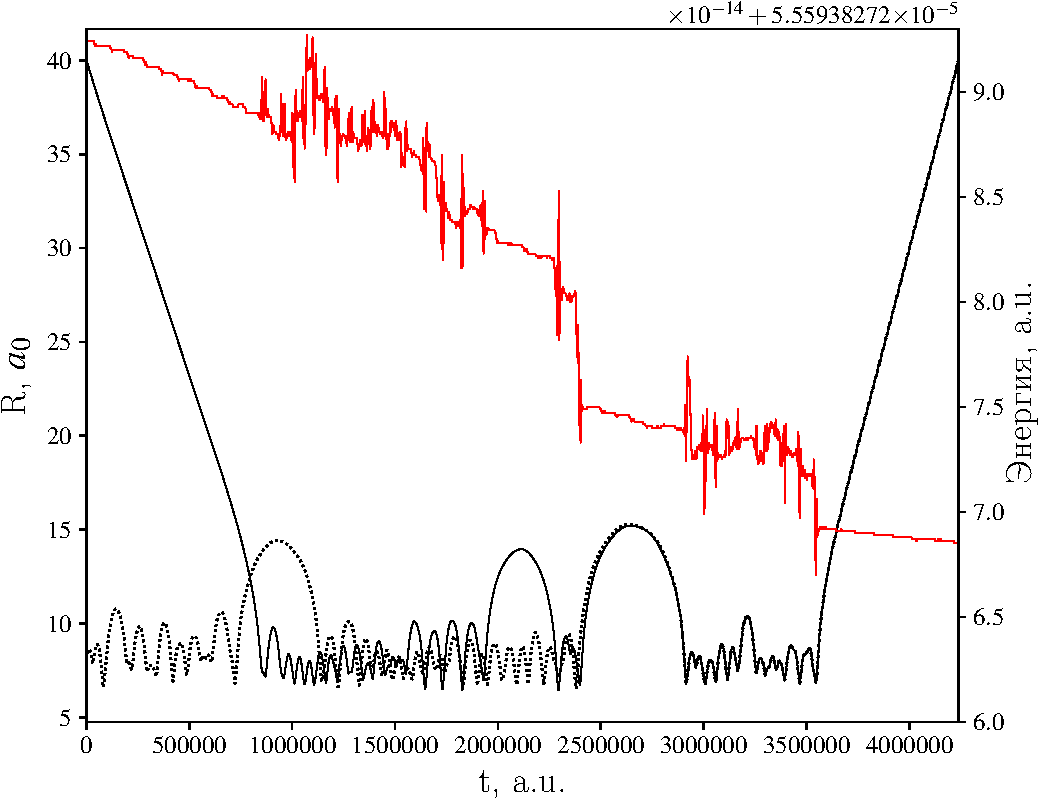
\includegraphics[width=0.85\linewidth]{./pictures/trajectories/euler_trajectory-crop.pdf}
\caption{Зависимости $R(t)$ для прямой (сплошная линия) и обратной (точечная линия) траекторий образования метастабильного комплекса N$_2-$N$_2$, полученные при решении полной системы динамических уравнений с углами и импульсами Эйлера \eqref{polyatom-euler-system}. Сверху отражено изменение энергии относительно начального значения вдоль прямой траектории со шкалой справа.}
    \label{fig:euler-trajectory}
\end{figure}

\subsection{Полная система динамических уравнений, записанная в компонентах углового момента}
    Полная система динамических уравнений с компонентами углового момента содержит два векторных уравнения Гамильтона относительно $\mf{q}$ и $\mf{p}$, дополненных обобщенным уравнением Эйлера, что в итоге приводит к системе из $2s + 3$ уравнений
\begin{gather}
    \begin{aligned}
        &\dot{\mf{q}} = \frac{\partial H}{\partial \mf{p}}, \\
        &\dot{\mf{p}} = -\frac{\partial H}{\partial \mf{q}}, \\
        &\dot{\mf{J}} + \Big[ \frac{\partial H}{\partial \mf{J}} \times \mf{J} \Big] = 0.
    \end{aligned}
\end{gather}

При подстановке колебательно-вращательного гамильтониана в форме \eqref{general-rovibrational-hamiltonian} приходим к следующему виду динамических уравнений
\begin{gather}
    \begin{aligned}
        &\dot{\mf{q}} = \bbG_{22} \mf{p} + \bbG_{12}^+ \mf{J}, \\
        &\dot{\mf{p}} = -\frac{1}{2} \mf{p}^+ \frac{\partial \bbG_{22}}{\partial \mf{q}} \mf{p} - \mf{J}^+ \frac{\partial \bbG_{12}}{\partial \mf{q}} \mf{p} - \frac{1}{2} \mf{J}^+ \frac{\partial \bbG_{11}}{\partial \mf{q}} \mf{J} - \frac{\partial U}{\partial \mf{q}}, \\
        &\dJx = \Jy \lb \bbG_{12} \mf{p} + \bbG_{11} \mf{J} \rb_z - \Jz \lb \bbG_{12} \mf{p} + \bbG_{11} \mf{J} \rb_y \\
        &\dJy = \Jz \lb \bbG_{12} \mf{p} + \bbG_{11} \mf{J} \rb_x - \Jx \lb \bbG_{12} \mf{p} + \bbG_{11} \mf{J} \rb_z \\
        &\dJz = \Jx \lb \bbG_{12} \mf{p} + \bbG_{11} \mf{J} \rb_y - \Jy \lb \bbG_{12} \mf{p} + \bbG_{11} \mf{J} \rb_x \\
    \end{aligned} \label{polyatom-jcomponents-system}
\end{gather}

Угловой момент $\mf{J}$ линейно связан с эйлеровыми импульсами согласно соотношению \eqref{polyatom-angular-momentum-euler-momenta}. При инверсии времени эйлеровы углы $\bUpsilon$ сохраняются, а эйлеровы импульсы меняют знак, следовательно, вектор углового момента также претерпевает инверсию  
\begin{gather}
    \mf{q}(t) = \mf{q}(-t), \quad \mf{p}(t) = -\mf{p}(-t), \quad \mf{J}(t) = -\mf{J}(-t).
\end{gather}

Начальные условия для траектории, представленной на рис. (\ref{fig:jcomponents-trajectory}), были пересчитаны из начальных условий траектории на рис. (\ref{fig:euler-trajectory}). 

\begin{figure}[H]
    \centering
    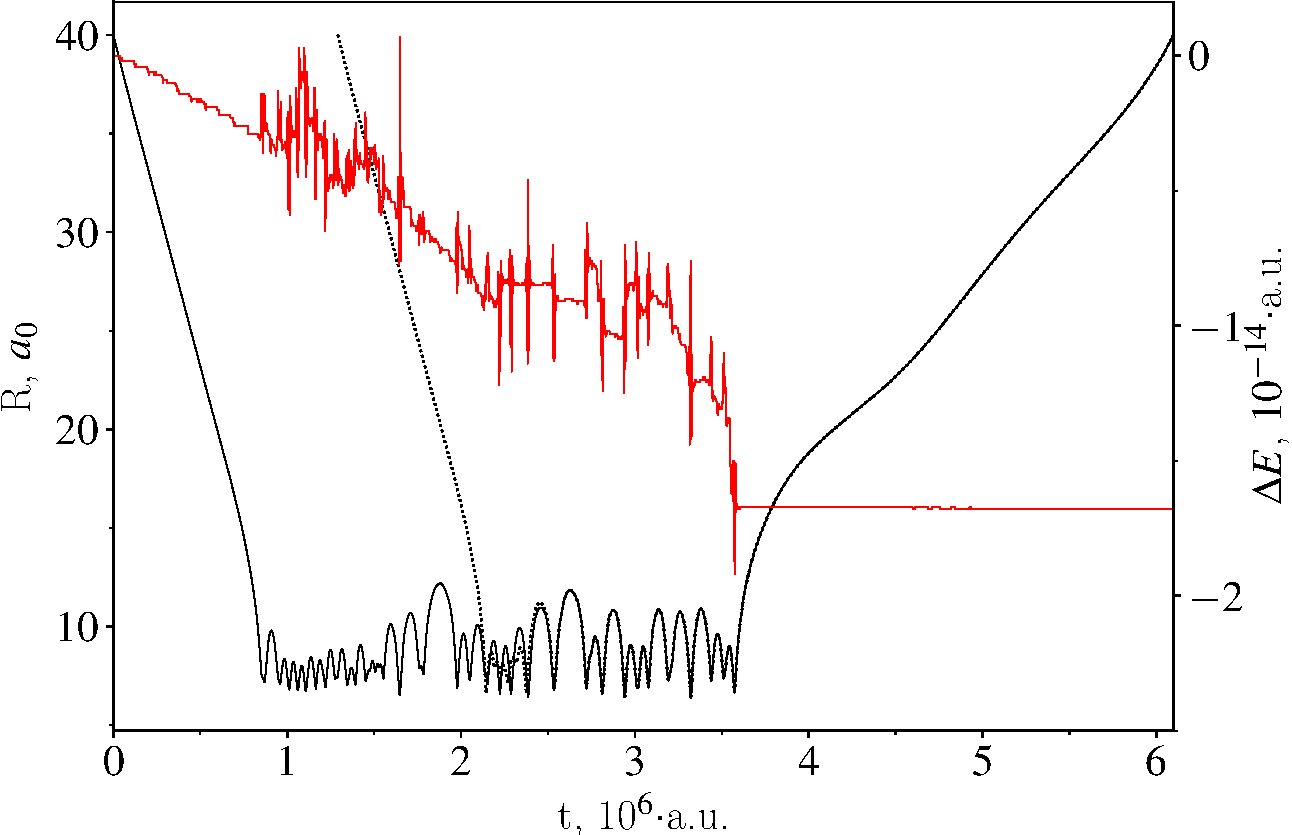
\includegraphics[width=0.85\linewidth]{./pictures/trajectories/jcomponents-trajectory-crop.pdf}
    \caption{Зависимости $R(t)$ для прямой (сплошная линия) и обратной (точечная линия) траекторий образования метастабильного комплекса N$_2-$N$_2$, полученные при решении полной системы динамических уравнений, записанной в декартовых компонентах углового момента \eqref{polyatom-jcomponents-system}. Сверху отражено изменение энергии относительно начального значения вдоль прямой траектории со шкалой справа.}
    \label{fig:jcomponents-trajectory}
\end{figure}


\subsection{Полная система динамических уравнений, учитывающая сохранение модуля вектора углового момента}
В этом случае система уравнений состоит из двух векторных уравнений Гамильтона относительно $\mf{q}$, $\mf{p}$, дополненных двумя уравнениями относительно сферических углов углового момента $\alpha$ и $\beta$, что в сумме приводит к системе из $2s + 2$ уравнений
\begin{gather}
    \begin{aligned}
        &\dot{\mf{q}} = \frac{\partial H}{\partial \mf{p}}, \\
        &\dot{\mf{p}} = -\frac{\partial H}{\partial \mf{q}}, \\
        &\dot{\alpha} = \frac{1}{J \sin \beta} \frac{\partial H}{\partial \beta}, \\
        &\dot{\beta} = -\frac{1}{J \sin \beta} \frac{\partial H}{\partial \alpha}.
    \end{aligned}
\end{gather}

Подставив колебательно-вращательный гамильтониан в форме \eqref{general-rovibrational-hamiltonian}, приходим к следующей системе уравнений
\begin{gather}
    \begin{aligned}
        &\dot{\mf{q}} = \bbG_{22} \mf{p} + \bbG_{12}^+ \mf{J}, \\
        &\dot{\mf{p}} = -\frac{1}{2} \mf{p}^+ \frac{\partial \bbG_{22}}{\partial \mf{q}} \mf{p} - \mf{J}^+ \frac{\partial \bbG_{12}}{\partial \mf{q}} \mf{p} - \frac{1}{2} \mf{J}^+ \frac{\partial \bbG_{11}}{\partial \mf{q}} \mf{J} - \frac{\partial U}{\partial \mf{q}}, \\
        &\dot{\alpha} = \frac{1}{J \sin \beta} \lsq \bbF \lb \bbG_{11} \mf{J} + \bbG_{12} \mf{p} \rb \rsq_y, \\
        &\dot{\beta} = -\frac{1}{J \sin \beta} \lsq \bbF \lb \bbG_{11} \mf{J} + \bbG_{12} \mf{p} \rb \rsq_z, 
    \end{aligned} \label{polyatom-jspherical-system}
\end{gather}
%
где компоненты вектора углового момента равны $\mf{J} = \lb J \cos \alpha \sin \beta, J \sin \alpha \sin \beta, J \cos \beta \rb$. \par
Исходя из того что при обращении времени происходит инверсия вектора углового момента, несложно получить следующие преобразования сферических углов вектора углового момента
\begin{gather}
    \mf{q}(t) = \mf{q}(-t), \quad \mf{p}(t) = -\mf{p}(-t), \quad \alpha(t) = \alpha(-t) - \pi, \quad \beta(t) = \pi - \beta(-t).
\end{gather}

Начальные условия для траектории, представленной на рис. (\ref{fig:jspherical-trajectory}), были пересчитаны из начальных условий траектории на рис. (\ref{fig:euler-trajectory}). 

\begin{figure}[H]
    \centering
    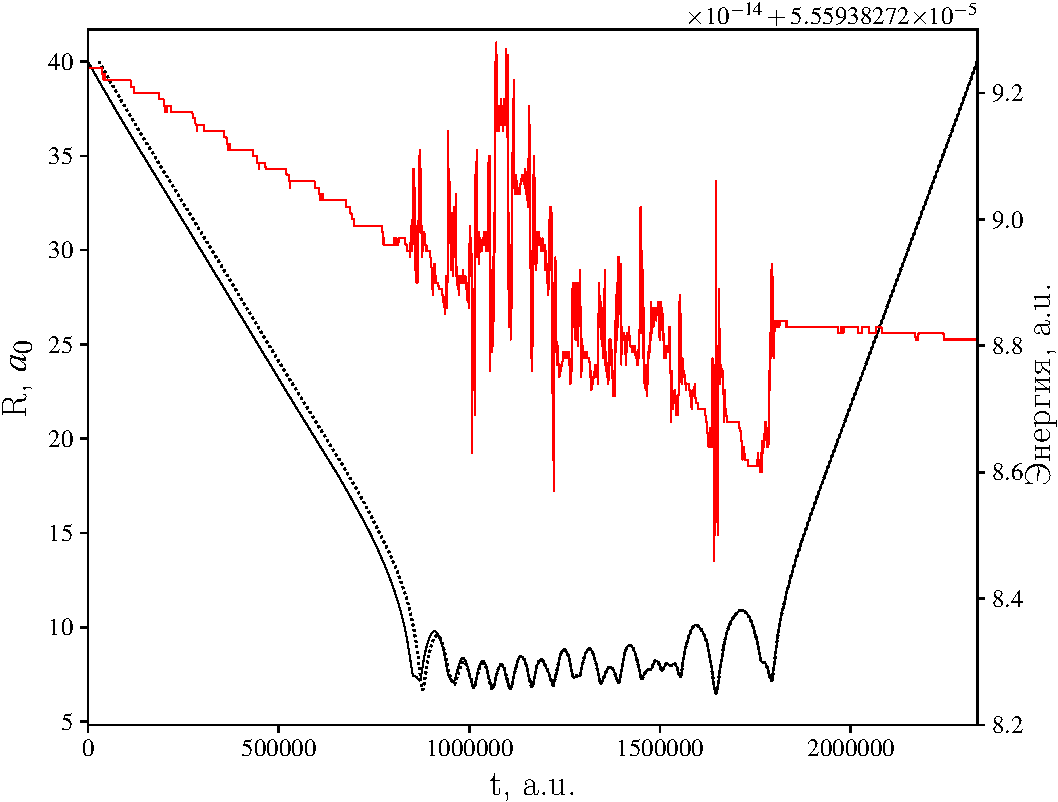
\includegraphics[width=0.85\linewidth]{./pictures/trajectories/spherical_trajectory-crop.pdf}
    \caption{Зависимости $R(t)$ для прямой (сплошная линия) и обратной (точечная линия) траекторий образования метастабильного комплекса N$_2-$N$_2$, полученные при решении полной системы динамических уравнений, учитывающей сохранение модуля вектора углового момента \eqref{polyatom-jspherical-system}. Сверху отражено изменение энергии относительно начального значения вдоль прямой траектории со шкалой справа.}
    \label{fig:jspherical-trajectory}
\end{figure}

На рис. (\ref{fig:trajectory-comparison}) представлено сравнение траекторий, пропагируемых в прямую сторону во времени, полученных при интегрировании трех разных систем уравнений. Мы видим, что интервал совпадения траекторий между собой сопоставим с интервалом совпадения прямой и обратной траекторий, полученных для каждой системы по отдельности. Таким образом, накопление численных ошибок происходит с сопоставимой скоростью для всех трех систем уравнений, поэтому никакую из систем нельзя выделить как более предпочтительную. \par
Отметим, что отклонение энергии от начального значения при решении любой из систем динамических уравнений имеет порядок $10^{-14}$ a.u. (или $\sym 10^{-9}$ см$^{-1}$), что говорит о высоком качестве получаемых траекторий.  

\begin{figure}[H]
    \centering
    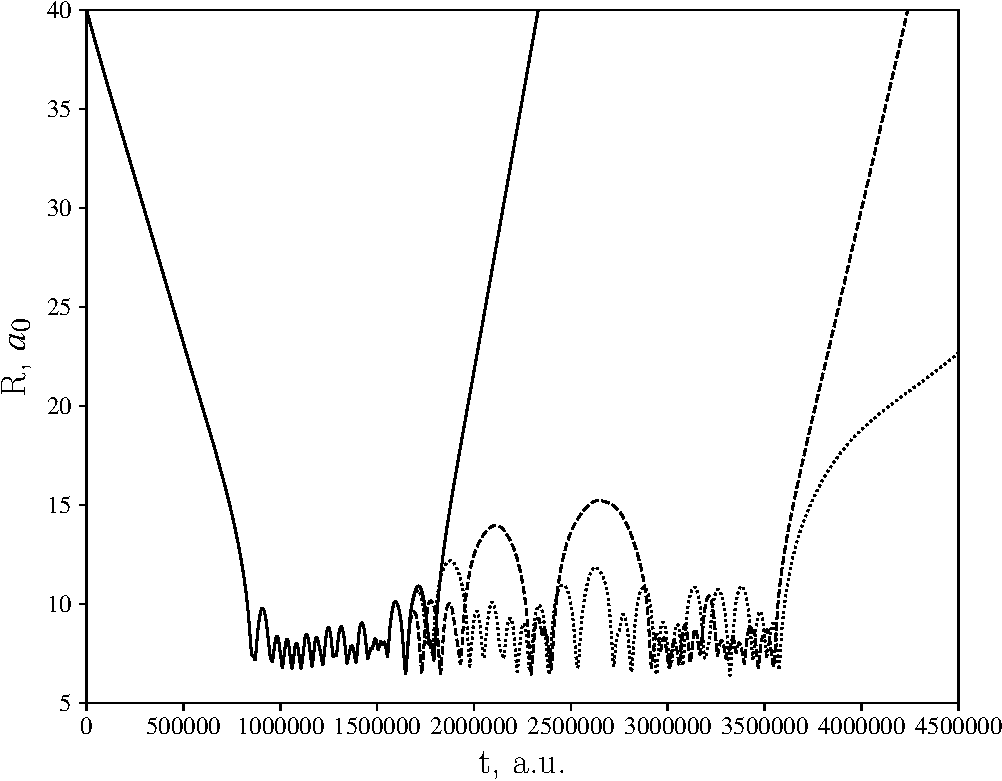
\includegraphics[width=0.85\linewidth]{./pictures/trajectories/trajectory-comparison-crop.pdf}
    \caption{Зависимости $R(t)$ траекторий образования метастабильного комплекса системы N$_2-$N$_2$, полученные при решении системы динамических уравнений с углами и импульсами Эйлера \eqref{polyatom-euler-system} (сплошная линия), системы с декартовыми компонентами углового момента \eqref{polyatom-jcomponents-system} (точечная линия) и системы, учитывающей сохранение модуля вектора углового момента \eqref{polyatom-jspherical-system} (пунктирная линия).}
    \label{fig:trajectory-comparison}
\end{figure}

Кроме того, при интегрировании траекторий на рис. (\ref{fig:trajectory-comparison}) были сделаны замеры количества промежуточных вычислений правых частей уравнений. Количество вызовов правых частей для пропагирования траекторий до фиксированного времени (1.500.000 атомных единиц времени) отличается не более чем на 1\%. Вычисление кинетической части для системы со сферическими углами углового момента \eqref{polyatom-jspherical-system} оказывается в среднем быстрее на 5-7\%, чем вычисление кинетической части для системы с декартовыми компонентами углового момента \eqref{polyatom-jcomponents-system}, а последняя, в свою очередь, на 5-7\% быстрее, чем кинетическая часть для системы с углами и импульсами Эйлера \eqref{polyatom-euler-system}. С ростом размерности системы скорость вычисления потенциальной части становится лимитирующим элементом при вычислении правых частей динамических уравнений, поэтому для больших систем скорости вычисления при использовании разных систем выравниваются. \par
При расчете спектральной функции по классической траектории требуется динамика вектора дипольного момента в лабораторной системе координат. Уравнения систем \eqref{polyatom-jspherical-system}, \eqref{polyatom-jcomponents-system} следует дополнить динамическим уравнением для эйлерового угла $\Phi$, т.к. два других угла Эйлера можно восстановить по вращению вектора углового момента в подвижной системе. Получив зависимости трех углов Эйлера от времени, можно преобразовать координаты вектора дипольного момента в молекулярной системе в координаты в лабораторной системе при помощи матрицы $\bbS$. Добавление еще одного уравнения к этим системам окончательно выравнивает вычислительную сложность всех систем, поэтому было принято решение для расчета массива траекторий использовать систему с углами и импульсами Эйлера, т.к. в этом случае легче реализуются вычислительные процедуры.

\section{Начальные условия для траекторного расчета}

Как и в случае двухатомных систем, в качестве начальных условий для траекторных расчетов мы будем использовать распределения с плотностью вероятности
\begin{gather}
    \rho(\mf{q}, \mf{p}) = \Gamma_0 \exp \lb -\frac{H(\mf{q}, \mf{p})}{kT} \rb
\end{gather}
%
при фиксированном расстоянии $\rfixed$ между центрами масс молекул, где постоянная $\Gamma_0$ определяется из условия нормировки
\begin{gather}
    \Gamma_0 \int \exp \lb -\frac{H(\mf{q}, \mf{p})}{k T} \rb d \mf{q} d\mf{p} = 1.
\end{gather}

Отметим, что мы хотим получить начальные распределения в области фазового пространства, определенной условием $H > 0$, то есть соответствующей свободным и метастабильным состояниям столкновительного комплекса. \par
В этой работе мы генерировали случайные величины из распределения $\rho(\mf{q}, \mf{p})$ при помощи метода Метрополиса-Хастингса \cite{liu2008}. Идея метода Метрополиса заключается в симуляции марковской цепи в фазовом пространстве, равновесное распределение точек которой совпадает с целевой функцией плотности вероятности. \par
Алгоритм предполагает генерацию последовательности случайных величин $\lc X_0 \right.$, $X_1$, $X_2, \dots \left. \rc$ (вектор $X_t$ включает в себя наборы координат $\mf{q}$ и импульсов $\mf{p}$). Последовательность обладает марковским свойством: для любого $t \geq 0$ следующий элемент последовательности выбирается с плотностью вероятности $T(X_{t +1} \vert X_t)$, не зависящей от предыдущего набора состояний $\lc X_0, X_1, \dots, X_{t - 1} \rc$. Для того чтобы плотность цепь Маркова асимптотически сходилась к целевому распределению, плотность вероятности $T$ должна быть симметричной 
\begin{gather}
    T(X_{t+1} \vert X_t) = T(X_t \vert X_{t+1}).
\end{gather}

Алгоритм состоит из нескольких простых шагов. Первым шагом алгоритма является выбор стартовой точки цепи. Ее выбор может определяться некоторым заданным исходным распределением, или же исходная точка может быть задана в каком-то фиксированном месте. Важно, чтобы стартовая точка не оказалась в \enquote{нефизичной} области пространства, потому что цепь может оказаться распределенной в малозначимом участке пространства. На практике цепь запускают по описанному ниже алгоритму в течение нескольких десятков тысяч шагов. Это позволяет цепи перейти в более вероятную область пространства, если начальное приближение было не самым удачным. Этот процесс иногда называют \enquote{разогревом} марковской цепи. \par
После выбора начальной точки из распределения $T$ выбирается потенциальная следующая точка $X_\text{next}$ цепи. Переход в выбранную точку $X_\text{next}$ из текущей точки $X_\text{current}$ происходит с вероятностью
\begin{gather}
    \alpha(X_\text{next} | X_\text{current}) = \min \lc 1, \frac{\rho(X_\text{next})}{\rho(X_\text{current})} \rc.
\end{gather}

С вычислительной точки зрения переход реализуется следующим образом. Генерируется случайное число с равномерной плотностью вероятности на отрезке $\lsq 0, 1 \rsq$. Если число оказывается меньшим, чем отношение плотности в потенциальной точке к плотности в текущей точке, то осуществляется переход. В противном случае -- переход считается неосуществленным и в качестве следующей точки цепи цепи выбирается текущая точка. \par
Заметим, что если плотность целевого распределения $\rho$ в потенциальной следующей точке $X_\text{next}$ больше, чем в текущей, то потенциальная точка принимается с единичной вероятностью. Однако, если плотность в потенциальной точке меньше, чем в текущей, то переход происходит с некоторой вероятностью, определяемой отношением плотностей. Таким образом, цепь с большей вероятностью переходит в участки пространства с большими значениями целевой плотности. В качестве плотности вероятности $T$ часто используют гауссовы функции, однако возможны и другие варианты. \par
Одна из основных проблем метода Метрополиса заключается в том, что метод по построению генерирует скоррелированные случайные величины. Для контроля скоррелированности получаемых значений цепи часто используют автокорреляционные функции. Скоррелированность значений можно контролировать при помощи параметров функции $T$. Существуют оптимальные параметры ширины распределения $T$, позволяющие уменьшить скоррелированность последовательных значений. Считается, что если частота переходов составляет 35-40\%, то параметры распределения $T$ выбраны удачно и динамика цепи происходит оптимально. Это утверждение не носит глобального характера, при генерации случайных величин из некоторых распределений оно может не выполняться. Кроме того, рекомендуемая частота переходов может сильно зависеть от размерности задачи. При построении марковских цепей в наших задачах мы обнаружили, что это значение частоты действительно является близким к оптимальному, поэтому производили подбор параметров функции $T$ так, чтобы частота переходов попала в оговоренный интервал. \par
Кроме того, для уменьшения корреляции выбираемых значений используют не каждое последующее значение в цепи, а значения, разделенные $K$ элементами. На практике $K$ варьируют от десятков до тысяч в зависимости от специфики задачи. Мы использовали значение $K$ порядка нескольких сотен. \par
Два репрезентативных примера распределений для обобщенных импульсов системы N$_2-$N$_2$  приведены на рис. (\ref{fig:polyatom-distributions}) для температур, при которых были сделаны траекторные расчеты спектров. В результате численной генерации распределений оказалось, что все импульсы, сопряженные полярному углу $\theta$, имеют гауссово распределение, а импульсы, сопряженные углу $\varphi$ -- распределение с острием (аналитическое выражение для плотности такого распределения было получено для двухатомной системы). Все полярные углы $\theta$ распределены равномерно с косинусом на интервале $\lsq 0, \pi \rsq$, а азимутальные углы $\varphi$ -- с равномерной плотностью на $\lsq 0, 2\pi \rsq$. Таким образом, все виды распределений, встречающихся для систем атом$-$линейная молекула и пара линейных молекул, уже встречались нам в двухатомных системах и были аналитически описаны. Однако выражения для параметров этих распределений через характеристики системы не были получены. Альтернативный способ генерации начальных условий, использующий приведение к диагональному виду кинетической энергии в форме Лагранжа, был предложен в дипломной работе \cite{chistikov-diplom}. \par 
Для системы N$_2-$N$_2$ в силу особенностей имеющейся аппроксимации потенциальной энергии максимальное расстояние было ограничено $30 a_0$. Это значение и было использовано при генерации начальных условий в качестве $\rfixed$. При этом межмолекулярном расстоянии могут быть найдены состояния, находящиеся в области $H < 0$, поэтому в ходе генерации цепи Маркова на каждом шаге делалась проверка знака гамильтониана в потенциальной следующей точке.
\setcounter{figure}{7}
\begin{figure}[H]
    \centering
    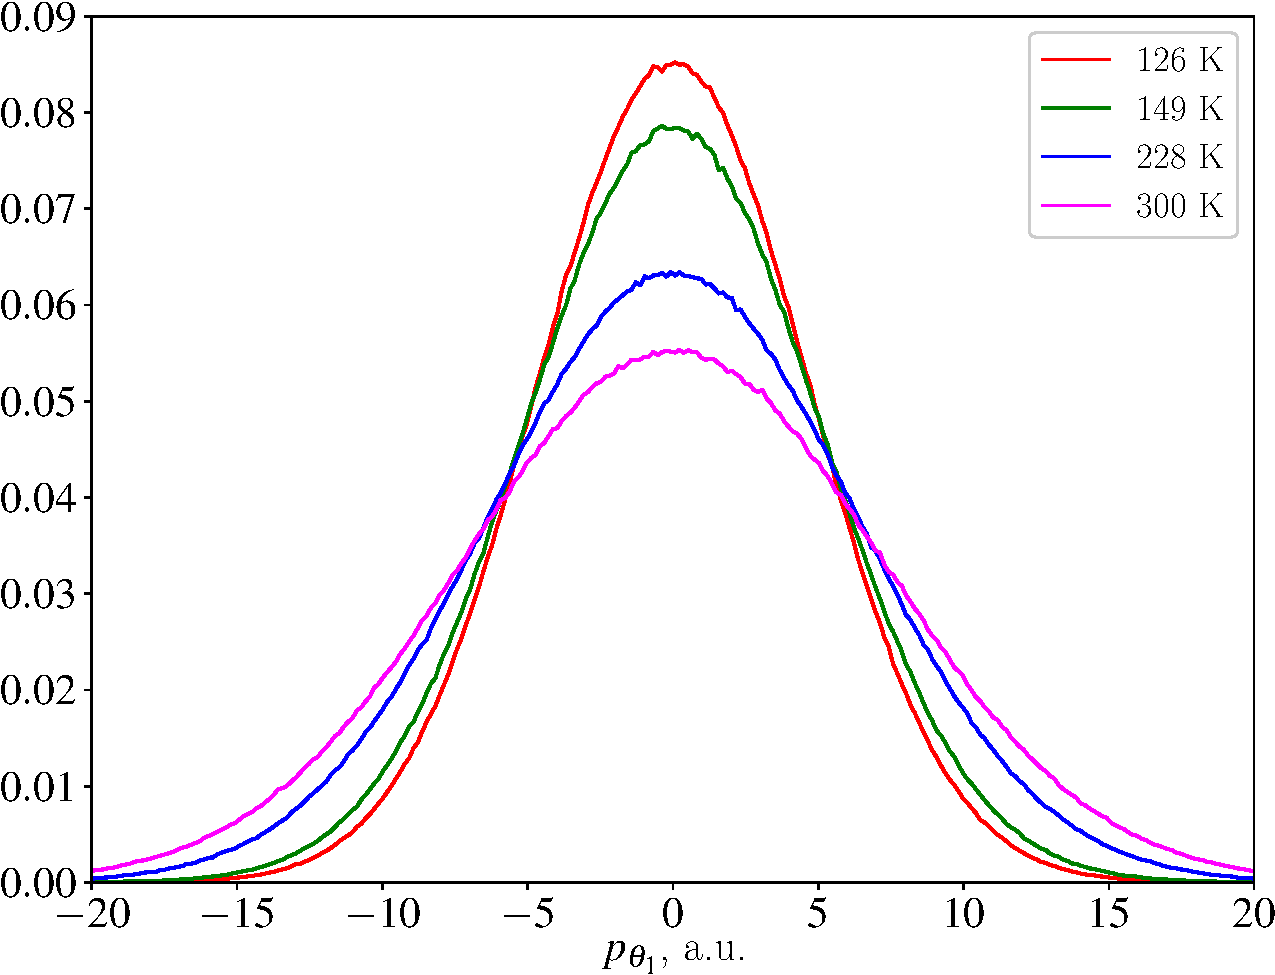
\includegraphics[width=0.75\linewidth]{./pictures/polyatom_distributions/pTheta1-crop.pdf} \\
    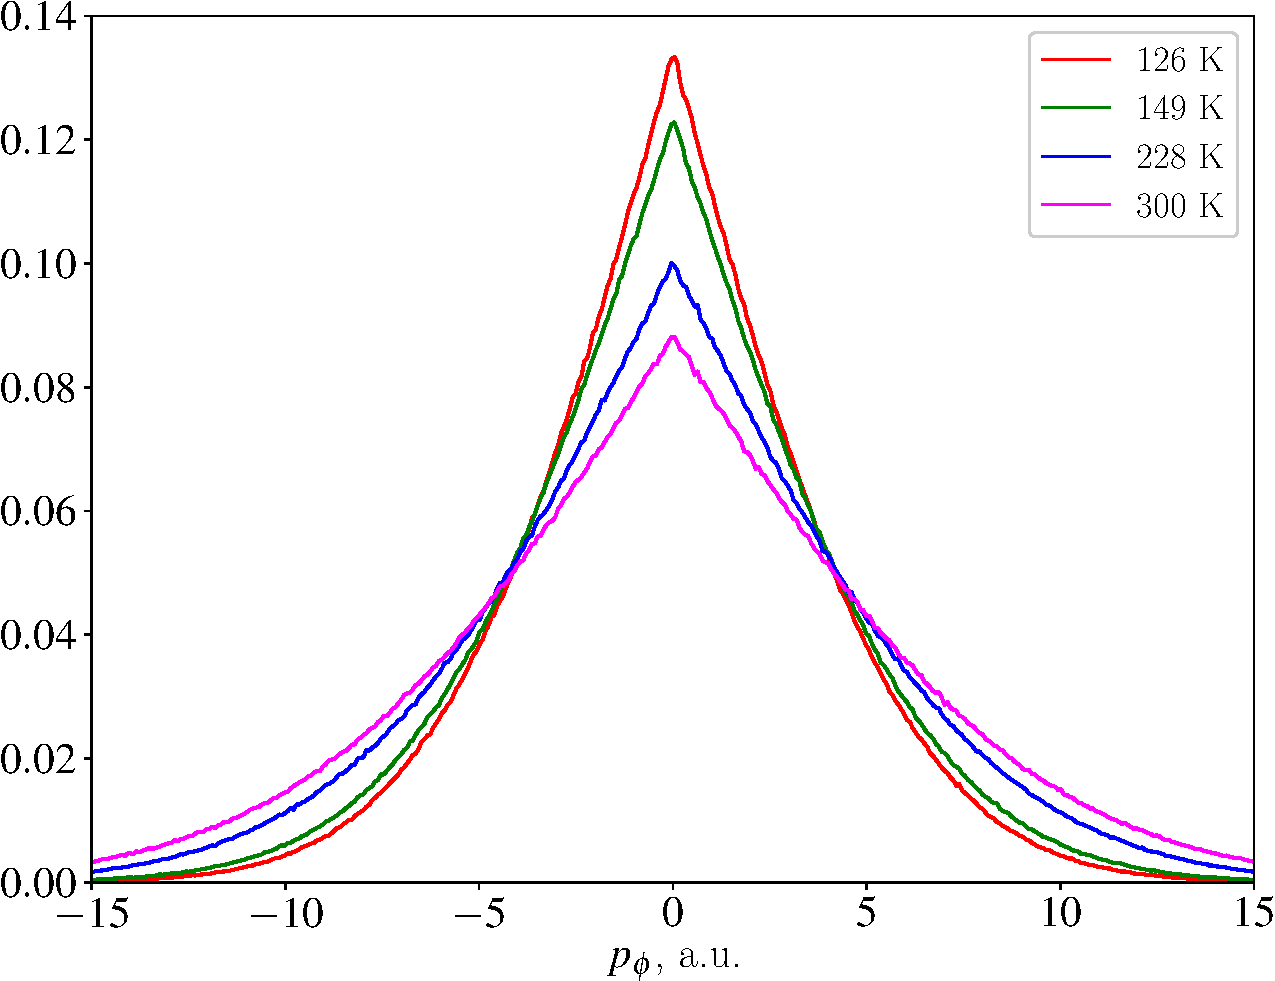
\includegraphics[width=0.75\linewidth]{./pictures/polyatom_distributions/pPhi-crop.pdf}
    \caption{Плотности распределений импульсов $p_{\theta_1}$ и $p_\varphi$ при температурах от 126К до 300К для системы N$_2-$N$_2$. Максимумы распределений убывают с увеличением температуры. Межмолекулярное расстояние $\rfixed$ взято равным 30 $a_0$. Количество сгенерированных точек при каждой температуре -- $N = 10^7$.}
    \label{fig:polyatom-distributions}
\end{figure}

\section{Проблемы, связанные с использованием подвижной системы отсчета}

Использование подвижной системы координат вызывает некоторые вычислительные проблемы при описании динамики столкновения молекул. \par
Рассмотрим движение системы атом$-$линейная молекула в отсутствии вращения молекулярной системы относительно лабораторной системы. Примем, что расстояние между атомом и линейной молекулой достаточно велико, и их взаимодействием можно пренебречь. Пусть линейная молекула претерпевает равномерное вращение относительно оси $OY$ подвижной системы. Заметим, что, когда линейная молекула и атом лежат на одной оси, подвижная система координат не определена. Более того, при каждом пересечении линейной молекулой оси $OZ$ подвижной системы изменяется направление осей $OX$ и $OY$. Это происходит, потому что угол $\theta$ определен от $0$ до $\pi$ и отсчитывается в положительную сторону направления оси $OX$. Поэтому при пересечении линейной молекулой оси $OZ$ ось $OX$ обязана изменить направление, а ось $OY$ определена так, чтобы тройка осей образовывала правую тройку. Описанная ситуация физически случается редко, однако если допустить вращение молекулярной системы, то эффект резкого поворота подвижной системы все равно будет наблюдаться. При резком вращении молекулярной системы, очевидно, существенно меняются производные эйлеровых импульсов, что вынуждает нас при численном решении системы использовать все меньшие шаги по времени. Однако размер шагов по времени ограничен снизу, и какие-то движения системы невозможно описать в рамках двойной точности. При расчете массива траекторий численное интегрирование таких траекторий обрывается, вклады таких траекторий в спектр не учитываются. Мы предполагаем, что траектории, на которых встречаются подобные вычислительные сложности, не локализованы в каких-то областях фазового пространтства и, следовательно, существенной погрешности в расчет суммарного спектрального профиля не вносят. \par
В случае пары двухатомных молекул возникает очень похожая ситуация. В этом случае плоскость подвижной системы координат $OXZ$ строится по одной из линейной молекул (будем называть ее первой) и центру масс второй линейной молекулы. Как и в предыдущем случае, подвижная система перестает быть определена, когда линейная молекула и центр масс второй молекулы лежат на одной прямой. Рассмотрим движение в отсутствие вращения подвижной системы координат. При равномерном вращении первой молекулы вокруг оси $OY$ подвижной системы происходит обращение осей $OX$ и $OY$, когда линейная молекула пересекает ось $OZ$. Возникают те же вычислительные сложности, что и в случае атом$-$линейная молекула. \par
В последнем случае, за счет большего количества атомов, можно сделать преобразование, существенно снижающее количество неопределенностей системы координат. Заметим, что резкие вращения подвижной системы происходят, только когда первая молекула (на которой \enquote{закреплена} плоскость подвижной системы) пересекает ось $OZ$, при этом движение второй молекулы может быть каким угодно. Если при подходе первой молекулы к оси $OZ$ осуществить перенос плоскости подвижной системы с первой молекулы на вторую, то движение первой молекулы не приведет к резкому вращению подвижной системы. Эта замена эквивалентна перенумерации молекул. Рассмотрим преобразование гамильтоновых переменных при перенумерации молекул. \par
Преобразование углов $\theta_1$, $\theta_2$ будет происходить по следующему закону, т.к. в результате перенумерации молекул изменяет свое направление ось $OZ$ подвижной системы
\begin{gather}
    \begin{aligned}
        \theta_1^\prime &= \pi - \theta_2, \\
        \theta_2^\prime &= \pi - \theta_1.
    \end{aligned}
\end{gather}

Преобразование эйлеровых углов $\Phi^\prime$, $\Theta^\prime$ происходит точно так же, как при инверсии декартовой тройки осей, относительно которых отсчитываются сферические углы. Понятно, что преобразование эйлерова угла $\Psi$ зависит от угла $\varphi$. Точный вид преобразования был подобран исходя из соображений инвариантности лагранжиана относительно осуществляемой замены:  
\begin{gather}
    \begin{aligned}
        \Phi^\prime &= \pi + \Phi, \\
        \Theta^\prime &= \pi - \Theta, \\
        \Psi^\prime &= \pi - \Psi - \varphi.
    \end{aligned}
\end{gather}

Получим преобразования скоростей при перенумерации молекул
\begin{gather}
    \begin{aligned}
        \dot{\theta}_1^\prime &= -\dot{\theta}_2, \\
        \dot{\theta}_2^\prime &= -\dot{\theta}_1, \\ 
        \dot{\Phi}^\prime &= \dot{\Phi}, \\
        \dot{\Theta}^\prime &= -\dot{\Theta}, \\
        \dot{\Psi}^\prime &= - \dot{\Psi} - \dot{\varphi}.
    \end{aligned} \label{polyatom-angles-exchange1}
\end{gather}

Получить аналогичные простые выражения для преобразования импульсов, сопряженных соотвествующим переменным, не представляется возможным, однако численно осуществить преобразование несложно. \par
Итак, пусть исходно мы имеем численные вектора обобщенных координат $\mf{q}$, сопряженных импульсов $\mf{p}$, вектор эйлеровых углов $\bUpsilon$ и эйлеровых импульсов $\pe$. Сначала рассчитаем лагранжевы скорости $\dot{\mf{q}}$ и $\dot{\boldsymbol{\Upsilon}}_e$ по соотношениям
\begin{gather}
    \begin{aligned}
        \dot{\boldsymbol{\Upsilon}}_e &= \bbW^+ \lb \bbG_{11} \bbW \pe + \bbG_{12} \mf{p} \rb, \\
        \dot{\mf{q}} &= \bbG_{12}^+ \bbW \pe + \bbG_{22} \mf{p}.
    \end{aligned}
\end{gather}

Предварительно для этого численно вычисляются матрицы $\bba$, $\bbA$, $\bbI$, и по формулам Фробениуса \eqref{polyatom-frobenius} рассчитываются матрицы $\bbG_{11}$, $\bbG_{12}$ и $\bbG_{22}$. Затем согласно полученным ранее соотношениям преобразуем лагранжевы переменные 

\begin{gather}
    \dot{\mf{q}}^\prime = 
    \begin{bmatrix}
        1 & 0 & 0 & 0 \\
        0 & 1 & 0 & 0 \\
        0 & 0 & 0 & -1 \\
        0 & 0 & -1 & 0 
    \end{bmatrix} \dot{\mf{q}}, \quad
    \dot{\boldsymbol{\Upsilon}}_e^\prime = 
    \begin{bmatrix}
        1 & 0 & 0 \\
        0 & -1 & 0 \\
        0 & 0 & -1
    \end{bmatrix}
    \dot{\boldsymbol{\Upsilon}}_e + 
    \begin{bmatrix}
        0 & 0 & 0 & 0 \\
        0 & 0 & 0 & 0 \\
        0 & -1 & 0 & 0 
    \end{bmatrix}
    \dot{\mf{q}}.
\end{gather}

После чего пересчитываем преобразованные лагранжевы переменные в гамильтоновы по соотношениям
\begin{gather}
    \begin{aligned}
        \mf{p}^\prime &= \bbA^+ \bbV \dot{\boldsymbol{\Upsilon}}_e^\prime + \bba \dot{\mf{q}}^\prime, \\
        \pe^\prime &= \bbV^+ \lb \bbI \bbV \dot{\boldsymbol{\Upsilon}}_e^\prime + \bbA \dot{\mf{q}}^\prime \rb, 
    \end{aligned}
\end{gather}
%
и продолжаем численное интегрирование траектории в преобразованных координатах $\mf{q}^\prime, \mf{p}^\prime, \bUpsilon^\prime$, $\pe^\prime$. \par
Понятно, что в тех случаях, когда все атомы линейных молекул выстраиваются вдоль одной линии, перенос подвижной системы не поможет. Численные расчеты показали, что доля таких траекторий имеет порядок $0.001 \%$. \par
В случае систем с большим количеством вращательных степеней свободы выбор подвижной системы становится шире, и, следовательно, снижается количество ситуаций, в которых невозможно определить подвижную систему. 

\section{Квантово-химические данные} \label{section:quantum-chemistry-data}

Поверхности потенциальной энергии и индуцированного дипольного момента для системы N$_2-$N$_2$ были взяты из работы \cite{karman2015}. Расчеты проводились с использованием метода связанных кластеров CCSD(T) в электронно-коррелированном базисе aug-cc-pVQZ. В полученных данных была учтена BSSE-коррекция. Дипольный момент комплекса рассчитывался методом конечного поля. Для устранения эффектов гиперполяризации в каждой геометрической конфигурации комплекса было проведено по 4 электронных расчета при разных напряженностях электрического поля. Расчеты были проведены при 29 разных взаимных ориентациях молекул и 15 разных значениях межмолекулярного расстояния. При избранных $T$-образных конфигурациях были проведены тестовые расчеты в базисе aug-cc-pV5Z. Наибольшая разница между значениями дипольного момента в двух базисах составила 0.3\%. \par
Аналитическая аппроксимация поверхности потенциальной энергии может быть выполнена в базисе сферических гармонических функций \cite{green1975} 
\begin{gather}
    V(R, \theta_1, \theta_2, \varphi) = \sum_{l_1, l_2, l} V_{l_1, l_2, l}(R) A_{l_1, l_2, l}(\theta_1, \theta_2, \varphi).
\end{gather}

Базисные функции $A_{l_1, l_2, l}(\theta_1, \theta_2, \varphi)$ являются произведениями присоединенных функций Лежандра $P^l_m(\theta)$
\begin{gather}
    A_{l_1, l_2, l}(\theta_1, \theta_2, \varphi) = \sqrt{\frac{2l+1}{4 \pi}} \Bigg[ \langle l_1 0 l_2 0 \vert l 0 \rangle P_{l_1}^0(\theta_1) P_{l_2}^0(\theta_2) + \hspace{5cm} \notag \\
    \hspace{4cm} + 2 \sum_{m} (-1)^m \langle l_1 m l_2 -m \vert l 0 \rangle P_{l_1}^m(\theta_1) P_{l_2}^m(\theta_2) \cos(m \varphi) \Bigg], 
\end{gather}
%
где через $\langle \cdots \vert \cdots \rangle$ обозначены коэффициенты Клебша-Гордона. Присоединенные функции Лежандра $P_l^m$ связаны со сферическими гармоническими функциями $Y_l^m$ соотношениями
\begin{gather}
    Y_l^m(\theta, \varphi) = P_l^m(\theta) e^{i m \varphi}.
\end{gather}

Вследствие того что обе молекулы являются гомоядерными, квантовые числа $l_1$ и $l_2$ принимают четные значения. \par
Коэффициенты разложения по угловому базису были найдены авторами \cite{karman2015} методом наименьших квадратов. Максимальные значения квантовых угловых чисел были взяты равными $l_1^\text{max} = l_2^\text{max} = 8$.  Радиальная зависимость коэффициентов углового базиса была аппроксимирована нами при помощи кубических сплайнов.  \par
Разложение дипольного момента $\bs{\mu}$ 
\begin{gather}
    \bs{\mu} = \lc
    \begin{aligned}
        \mu_x &= \frac{\mu^{-1} - \mu^{+1}}{\sqrt{2}} \\
        \mu_y &= \frac{\mu^{+1} - \mu^{-1}}{i \sqrt{2}} \\
        \mu_z &= \mu^0
    \end{aligned}
    \right.
\end{gather}
%
часто записывается в угловых координатах, определенных в лабораторной системе координат. Компоненты $\mu^{0, \pm 1}$ могут быть разложены в базисе сферических функций согласно следующим формулам \cite{hartmann2011} 
\begin{gather}
    \mu^n (n = 0, \pm 1) = \frac{( 4 \pi )^{3/2}}{\sqrt{3}} \sum_{l_1, l_2, \Lambda, l} A_{l_1, l_2, \Lambda, l}(R) \sum_{m_\Lambda, m, m_1, m_2} (-1)^{l_1 + l_2 + m_\Lambda + \Lambda + l + n} \sqrt{3 (2\Lambda + 1)} \times \notag \\
    \times
    \begin{pmatrix}
        \Lambda & l & 1 \\ m_\Lambda & m & -n 
    \end{pmatrix}
    \begin{pmatrix}
        l_1 & l_2 & \Lambda \\
        m_1 & m_2 & -m_\Lambda
    \end{pmatrix}
    Y_{l_1}^{m_1}(\theta_1, \varphi_1) Y_{l_2}^{m_2}(\theta_2, \varphi_2) Y_l^m(\theta, \varphi), \label{dipole-expansion} 
\end{gather}
%
где через $(:::)$ обозначены 3j-символы Вигнера. Наборы углов $(\theta_1, \varphi_1)$, $(\theta_2, \varphi_2)$ и $(\theta, \varphi)$ описывают относительную ориентацию первой, второй молекулы и межмолекулярной оси, соответственно. Разложение \eqref{dipole-expansion} следует преобразовать к угловым координатам молекулярной системы координат, детально эти преобразования описывать не будем. \par
Коэффициенты разложения по угловому базису также были найдены методом наименьших квадратов, здесь размер углового базиса был ограничен максимальными значениями квантовых угловых чисел $l_1^\text{max} = l_2^\text{max} = 6$. Радиальная зависимость коэффициентов углового базиса также была аппроксимирована при помощи кубических сплайнов. \par
Глобальный минимум поверхности потенциальной энергии достигается в \enquote{скошенной} конфигурации; глубина потенциальной ямы составляет около 100 см$^{-1}$ (рис. \ref{fig:n2n2-potential-curves}). Близко к глобальному минимуму расположен минимум в $T$-образной конфигурации, которая обладает наибольшим дипольным моментом. \enquote{Скошенная} конфигурация, являясь высокосимметричной, не обладает дипольным моментом. 

\setcounter{figure}{8}
\begin{figure}[H]
    \centering
    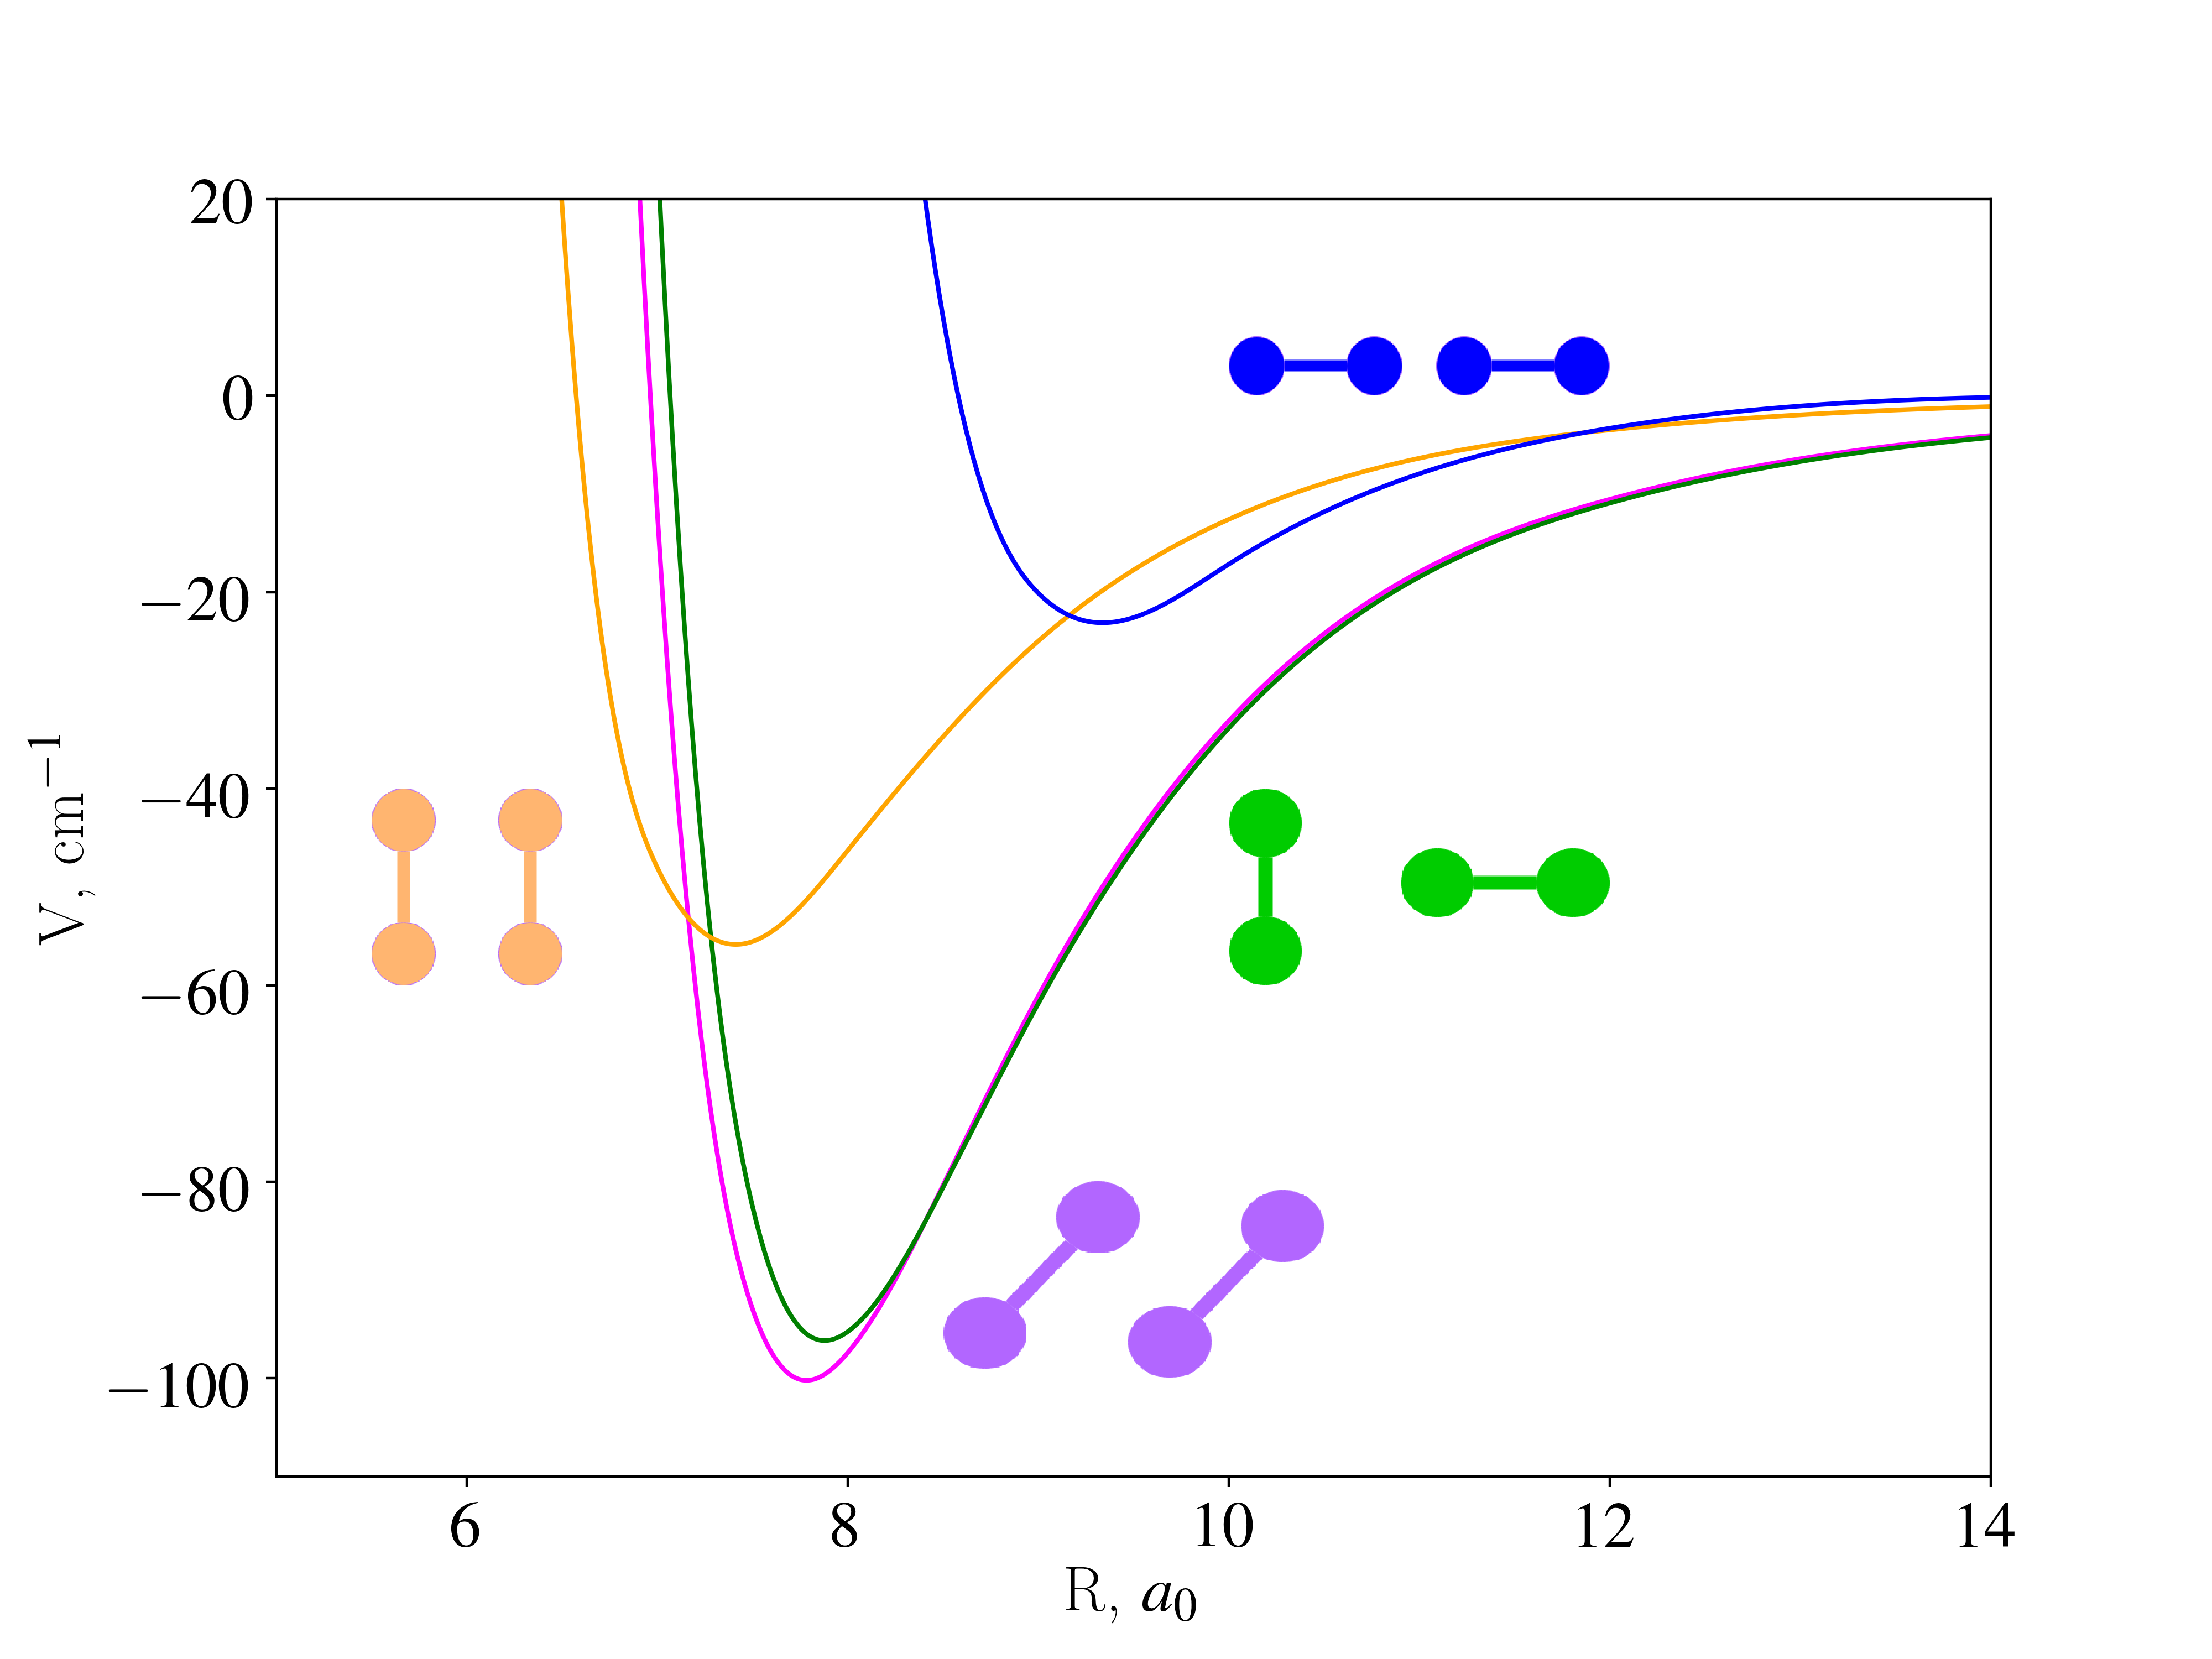
\includegraphics[width=0.75\linewidth]{./pictures/n2n2_potential.png}
    \caption{Радиальные зависимости потенциальной энергии системы N$_2-$N$_2$ в нескольких угловых конфигурациях}
    \label{fig:n2n2-potential-curves}
\end{figure}

Поверхности потенциальной энергии и индуцированного дипольного момента для системы CO$_2-$Ar были заимствованы из \cite{julia}. Для расчетов использовался метод связанных кластеров CCSD(T), являющийся \enquote{золотым стандартом} в этом классе задач. При расчете обеих поверхностей использовался электронно-коррелированный базис aug-cc-pVTZ, дополненный связевыми функциями. В полученных данных была скорректирована BSSE-ошибка. \par
Аналитическая аппроксимация поверхности потенциальной энергии была выполнена в базисе полиномов Лежандра
\begin{gather}
    V(R, \theta) = \sum_{\lambda = 0}^{\lambda^\text{max}} V_\lambda(R) P_\lambda(\cos \theta). \label{co2-ar-expansion}
\end{gather}

В силу симметричности молекулы CO$_2$ в разложении \eqref{co2-ar-expansion} присутствуют только четные $\lambda$. Максимальное значение квантового числа $\lambda$ было взято равным $\lambda^\text{max} = 10$. Радиальные функции $V_\lambda(R)$ были описаны сплайнами на средних расстояниях, экспонентой -- на малых расстояниях и полиномиальными функциями -- при больших расстояниях. \par
Аналитическое представление поверхности дипольного момента может быть выполнено в базисе присоедиенных функций Лежандра. При описании системы, закрепленной в плоскости $OXZ$ подвижной системы координат, $y$-компонента дипольного момента равна нулю, а $x$- и $z$-компоненты могут быть разложены в ряды \cite{meyer1986_h2he}
\begin{gather}
    \mu_x = \sum_{\lambda = 1}^{\lambda^\text{max}} \alpha_\lambda(R) P_\lambda^1(\cos \theta), \quad \mu_z = \sum_{\lambda_1}^{\lambda^\text{max}} \beta_\lambda(R) P_\lambda^0(\cos \theta).
\end{gather}

\begin{figure}[H]
    \centering
    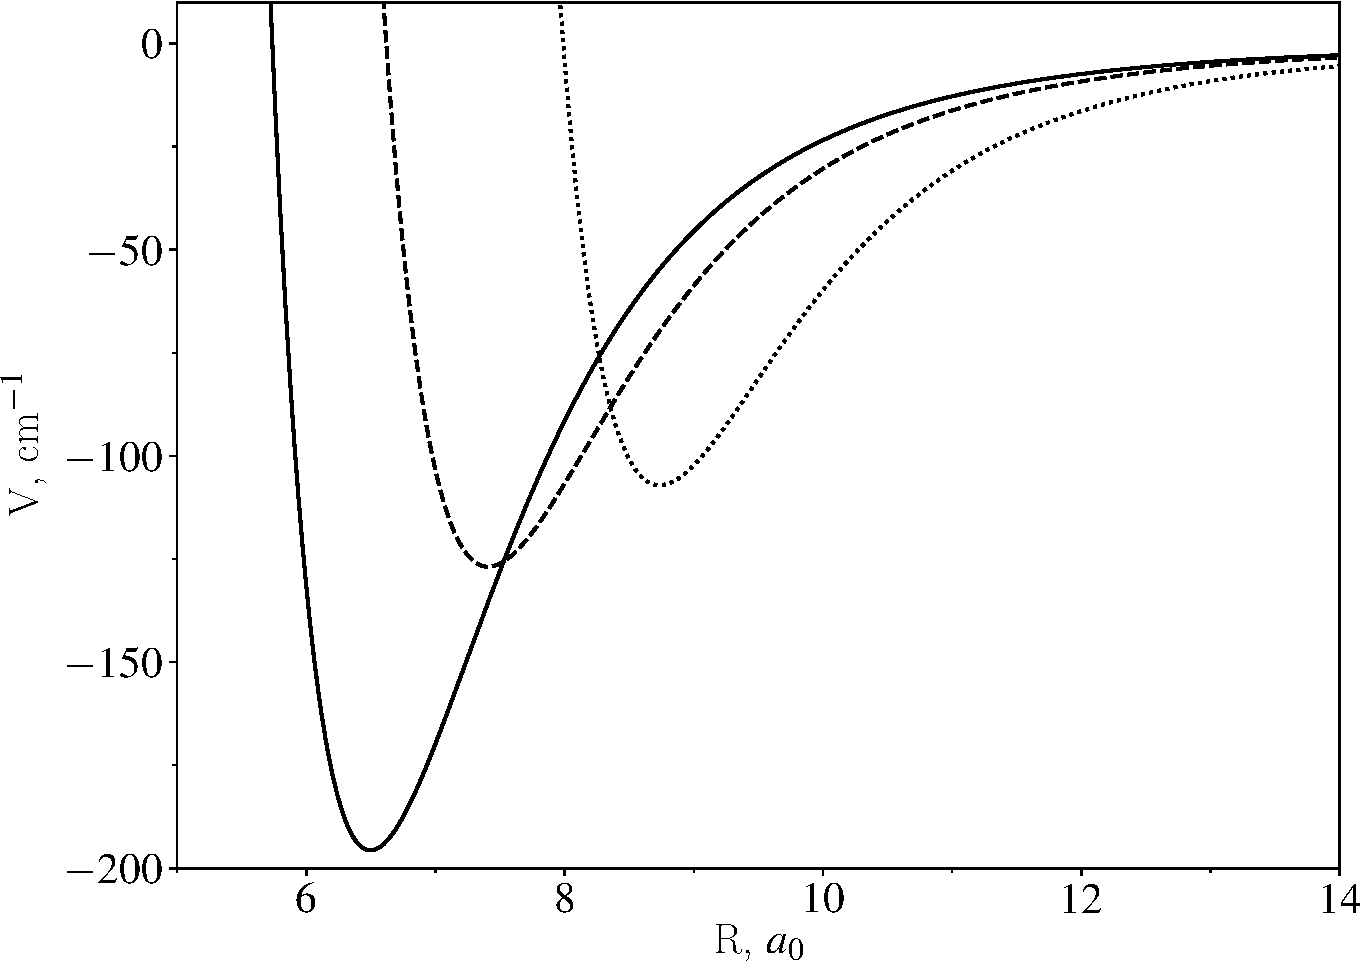
\includegraphics[width = 0.75\linewidth]{./pictures/co2-ar-potential-crop.pdf}
    \label{fig:co2-ar-potential}
    \caption{Сечения поверхности потенциальной энергии системы CO$_2-$Ar. Сплошной линией обозначена радиальная зависимость при $\theta = \pi/2$, пунктиром -- при $\theta = \pi/3$, точками -- при $\theta = 0$.}
\end{figure}

Глобальный минимум поверхности составляет примерно 196 см$^{-1}$ и достигается при $T$-образной конфигурации комплекса.

\section{Результаты траекторных расчетов}

Было предположено, что выражение для спектральной функции \eqref{two-atom-spectral-function4} обобщается на многомерные системы (то есть что появление множитель $p_r/ \mu$ связано с переходом от интеграла по $dr$ к интегралу по $dt$ и не зависит от количества угловых переменных). Здесь $\mu$ обозначает приведенную массу комплекса как квазидвухатомной системы:
\begin{gather}
    \mu = \frac{m_1 m_2}{m_1 + m_2},
\end{gather}
%
где $m_1$, $m_2$ -- массы первой и второй молекулы, соответственно. \par
Обобщение \eqref{two-atom-spectral-function4} на многомерные системы выглядит следующим образом
\begin{gather}
    V J(\omega) =  \frac{V}{4 \pi \varepsilon_0} \frac{1}{2\pi \Gamma_0}\int_0^\infty \frac{p_r}{\mu} dp_r \int \exp \lb -\frac{H}{\kb T} \rb d\mf{q}^\prime d\mf{p}^\prime d\bUpsilon d\pe \Bigg\vert \intty \bs{\mu}(t) e^{-i \omega t} dt \Bigg\vert^2, \label{polyatom-spectral-function1} 
\end{gather}
%
где $d\mf{q}^\prime$ содержит дифференциалы только угловых координат, а $d\mf{p}^\prime$ -- дифференциалы импульсов, сопряженных угловым координатам. Строго переход от интеграла по $dr$ к интегралу по $dt$ для многоатомных систем обоснован не был, однако результаты численных экспериментов показывают, что выражение \eqref{polyatom-spectral-function1} является верным. \par
Интегрирование в \eqref{polyatom-spectral-function1} производилось методом Монте-Карло с весовой функцией $p_\xi(\bxi) = \exp \lb - H(\bxi)/\kb T \rb / \Gamma_1$, где $\bxi = \lb p_r, \mf{p}^\prime, \bUpsilon, \pe \rb$, а $\Gamma_1$ -- нормировочный множитель, равный
\begin{gather}
    \Gamma_1 = \int_0^\infty dp_r \int \exp \lb -\frac{H}{\kb T} \rb d\mf{q}^\prime d\mf{p}^\prime d\bUpsilon d\pe.
\end{gather}

Рассмотрим выражение \eqref{polyatom-spectral-function1} как математическое ожидание квадрата преобразования Фурье на распределении $\bxi$
\begin{gather}
    VJ(\omega) = \frac{V}{4 \pi \varepsilon_0} \frac{\Gamma_1}{2 \pi \Gamma_0} \lim_{N \rightarrow \infty} \frac{1}{N} \sum_{k = 1}^N \frac{p_r(\bxi_k)}{\mu} \Bigg\vert \intty \bs{\mu}(t; \bxi_k) e^{-i \omega t} dt \Bigg\vert^2,
\end{gather}
%
где используются те же обозначения, что и в выкладках для системы двух атомов. Несложно показать, что отношение нормировочных интегралов в общем случае будет равным
\begin{gather}
    \frac{V \Gamma_1}{2 \pi \Gamma_0} = \rfixed^2.
\end{gather}

Следовательно, итоговое выражение для спектральной функции как среднего по распределению $\bxi$ в многомерном случае выглядит таким же образом, как и для системы двух атомов:
\begin{gather}
    V J(\omega) = \frac{\rfixed^2}{4 \pi \varepsilon_0} \lim_{N \rightarrow \infty} \frac{1}{N} \sum_{k = 1}^N \frac{p_r(\bxi_k)}{\mu} \Bigg\vert \intty \bs{\mu}(t; \bxi_k) e^{-i \omega t} dt \Bigg\vert^2. \label{polyatom-spectral-function2}
\end{gather}

\setcounter{figure}{10}
\begin{figure}[H]
    \centering
    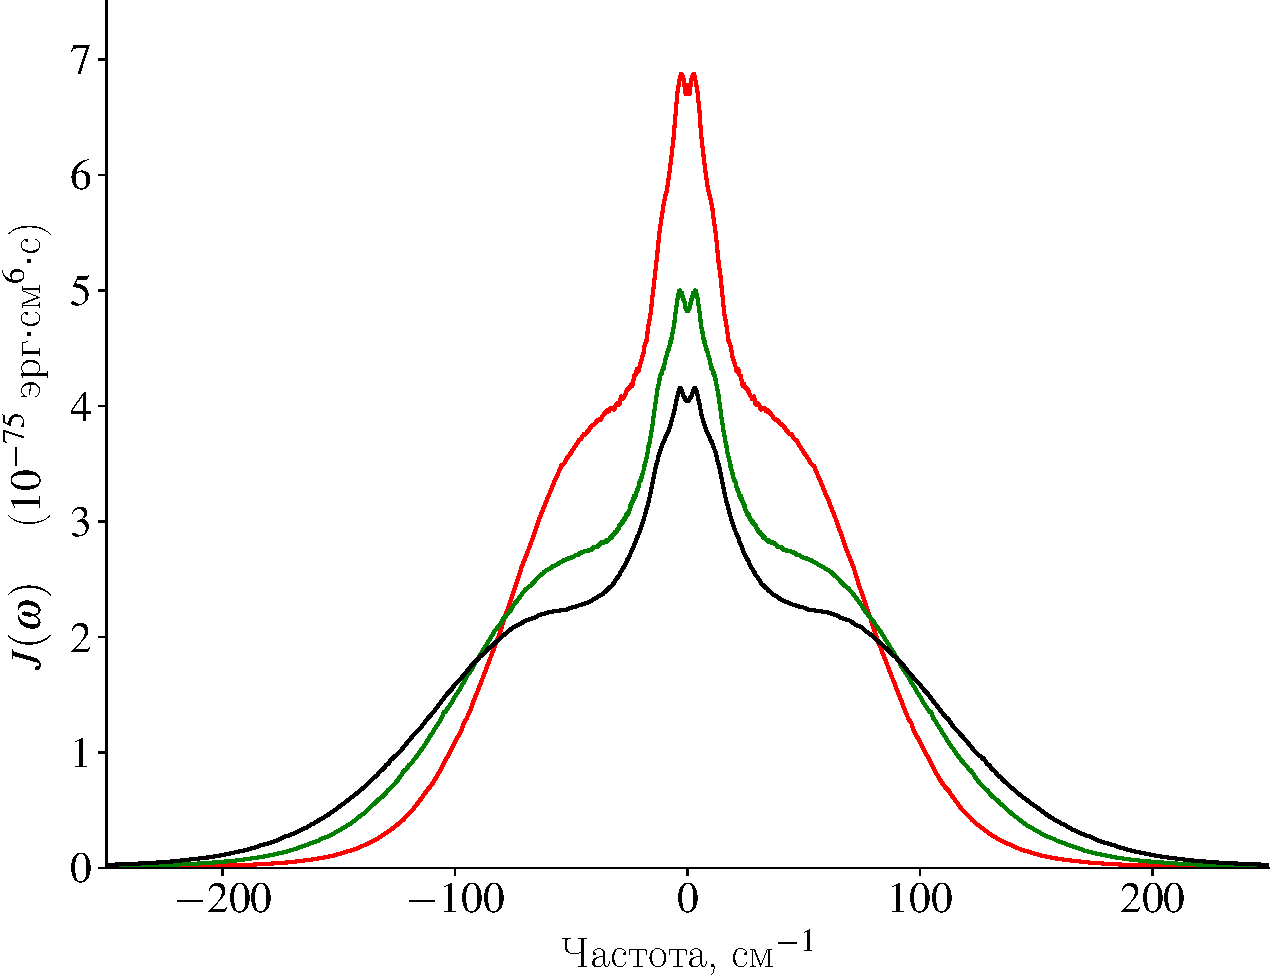
\includegraphics[width=0.7\linewidth]{./pictures/polyatom_spectra/n2n2_spectral_functions-crop.pdf}
    \caption{Классические спектральные функции системы N$_2-$N$_2$ при температурах 149К (верхняя красная кривая), 228К (средняя зеленая кривая) и 300К (нижняя черная кривая).}
    \label{fig:n2n2-spectral-functions}
\end{figure}

Для сравнения с экспериментальными данными спектральная функция, полученная по \eqref{polyatom-spectral-function2},  подвергалась процедуре десимметризации D3 \eqref{d3}. Для систем CO$_2-$Ar и N$_2-$N$_2$ влияние процедуры десимметризации достаточно велико даже при комнатной температуре, что продемонстрировано на рисунке \ref{fig:n2n2-desymmetrization}. 

\begin{figure}[H]
    \centering
    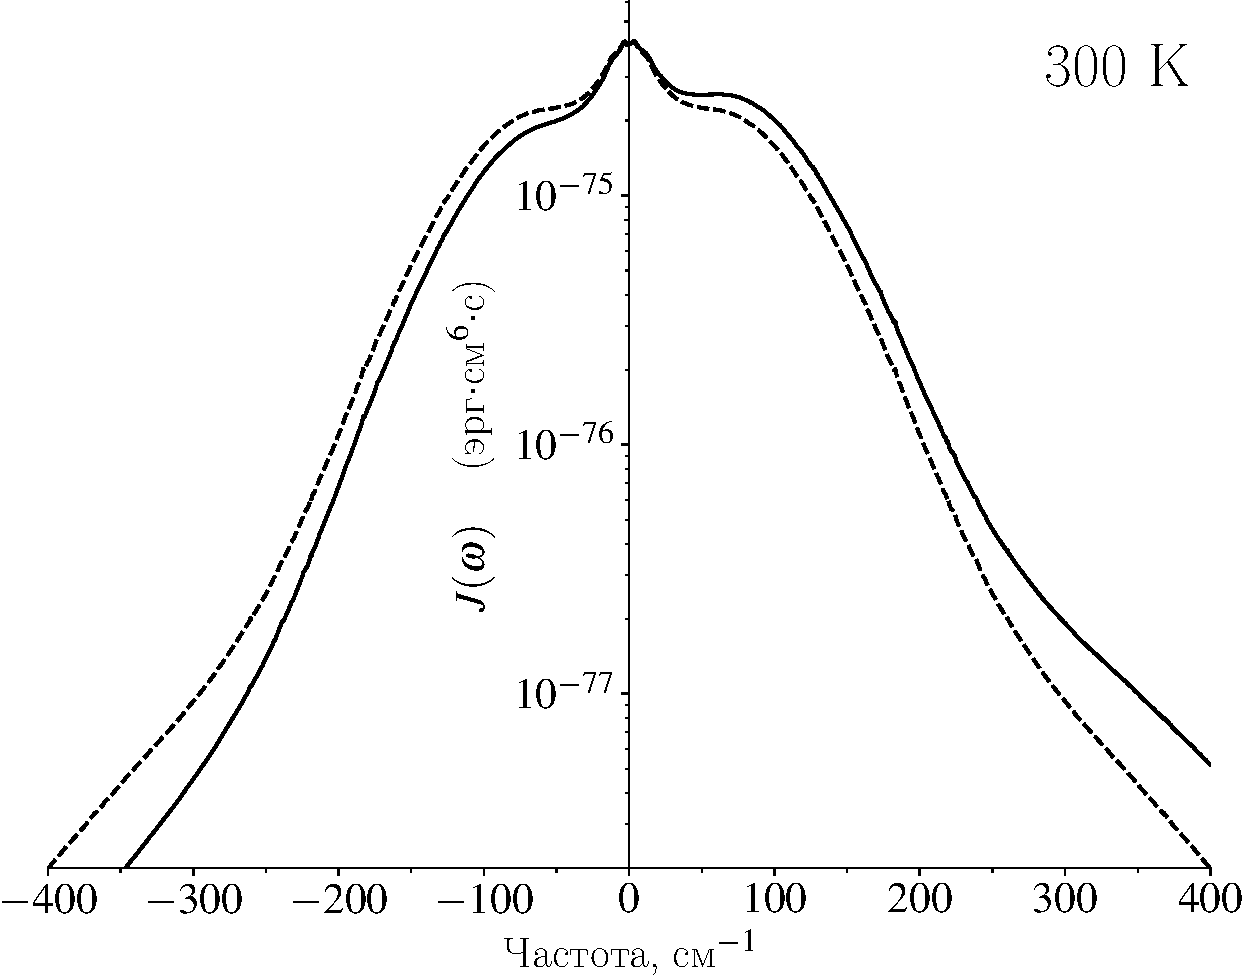
\includegraphics[width=0.49\linewidth]{./pictures/polyatom_spectra/n2n2_spectral_function_300K-crop.pdf}
    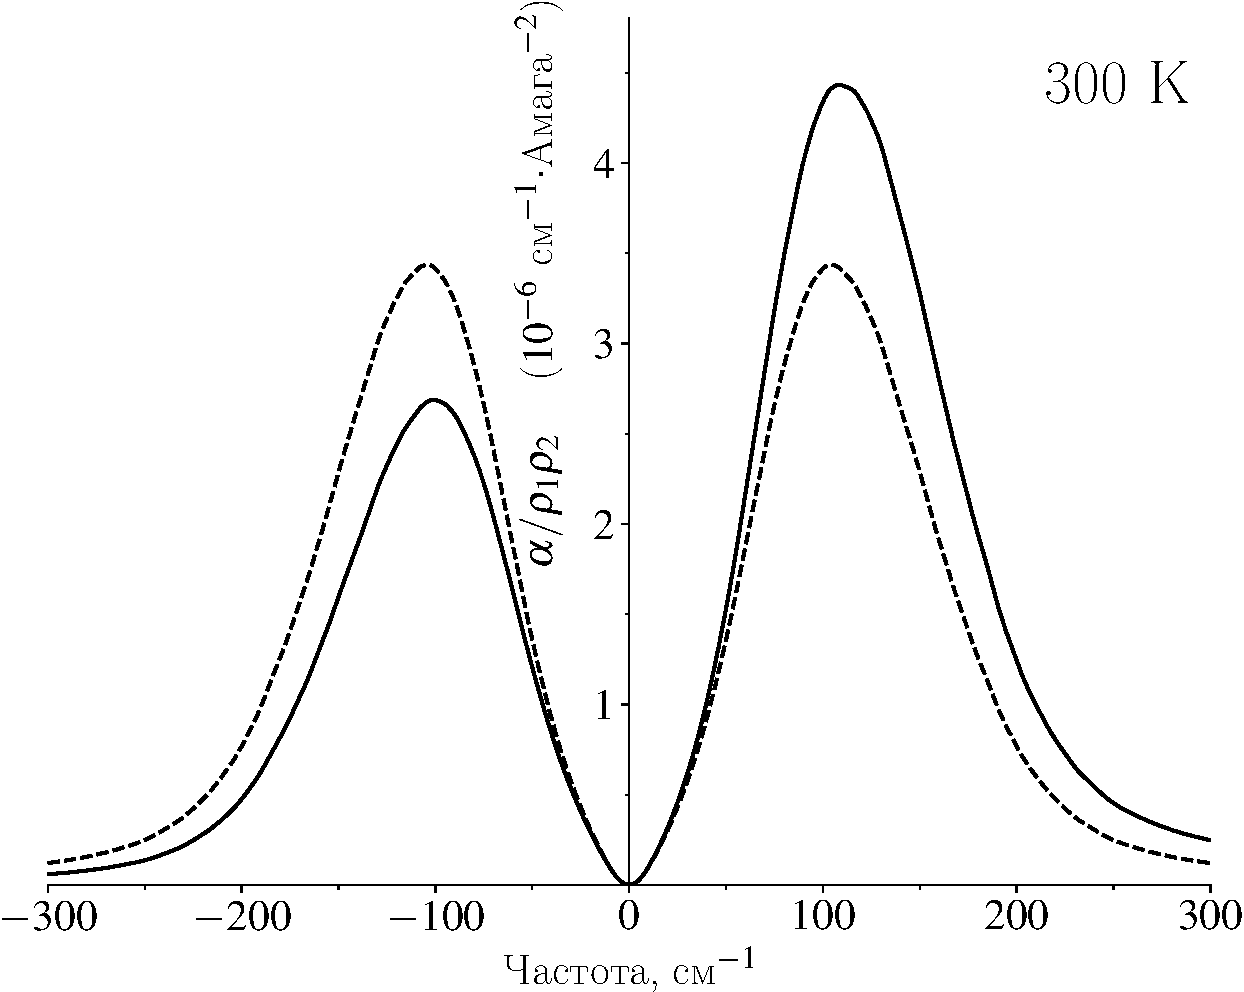
\includegraphics[width=0.49\linewidth]{./pictures/polyatom_spectra/n2n2_desymmetrization-crop.pdf}
    \caption{Влияние десиметризации на спектральную функцию и спектральный профиль на примере спектральной функции системы N$_2-$N$_2$ при 300К. Пунктиром обозначены классические спектральные функция и профиль; сплошной линией -- полученные из классических в результате применения процедуры D3.}
    \label{fig:n2n2-desymmetrization}
\end{figure}

На рис. (\ref{fig:n2n2-spectra}) представлено сопоставление рассчитанных спектральных профилей системы N$_2-$N$_2$ с другими расчетными и экспериментальными данными. В таблице (\ref{table:n2n2-spectra}) представлены численные значения коэффициентов поглощения, представленные на рис. (\ref{fig:n2n2-spectra}). 

\begin{figure}[H]
    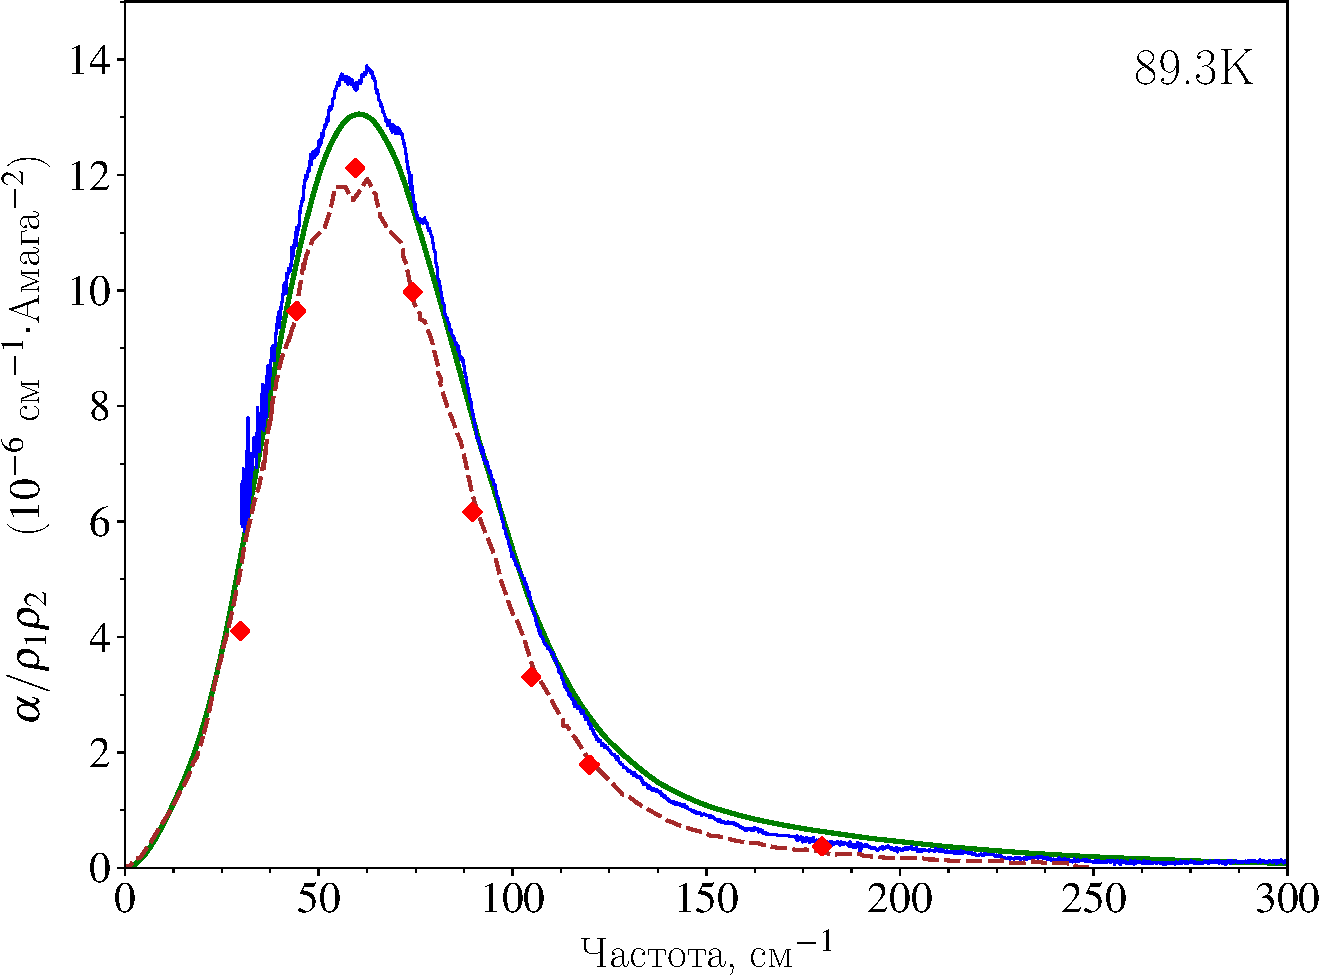
\includegraphics[width=0.49\linewidth]{./pictures/polyatom_spectra/89_3K_russian-crop.pdf} 
    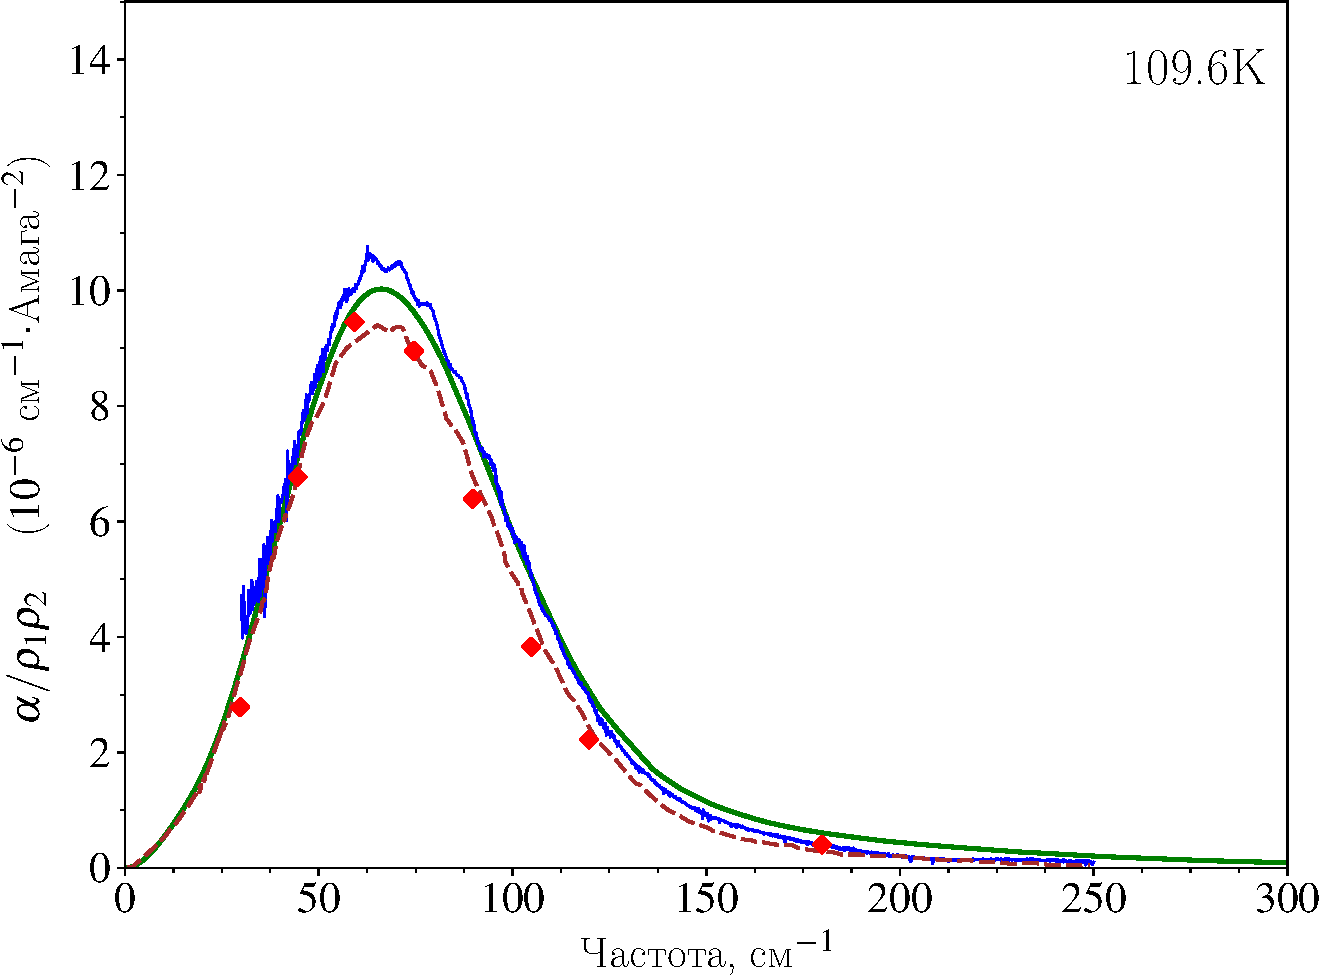
\includegraphics[width=0.49\linewidth]{./pictures/polyatom_spectra/109_6K_russian-crop.pdf} \\ 
    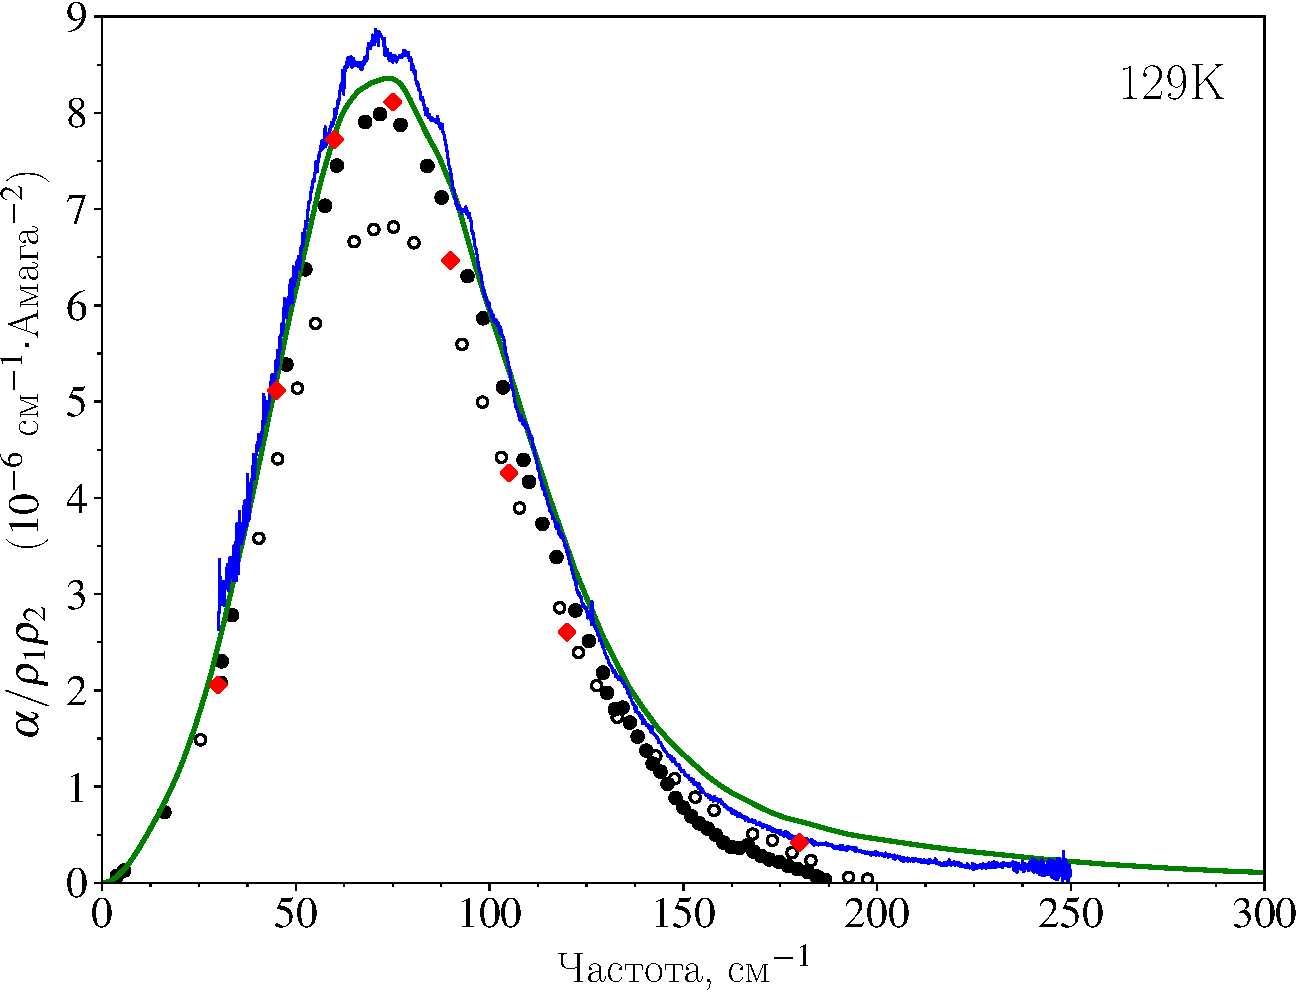
\includegraphics[width=0.49\linewidth]{./pictures/polyatom_spectra/129K_russian-crop.pdf} 
    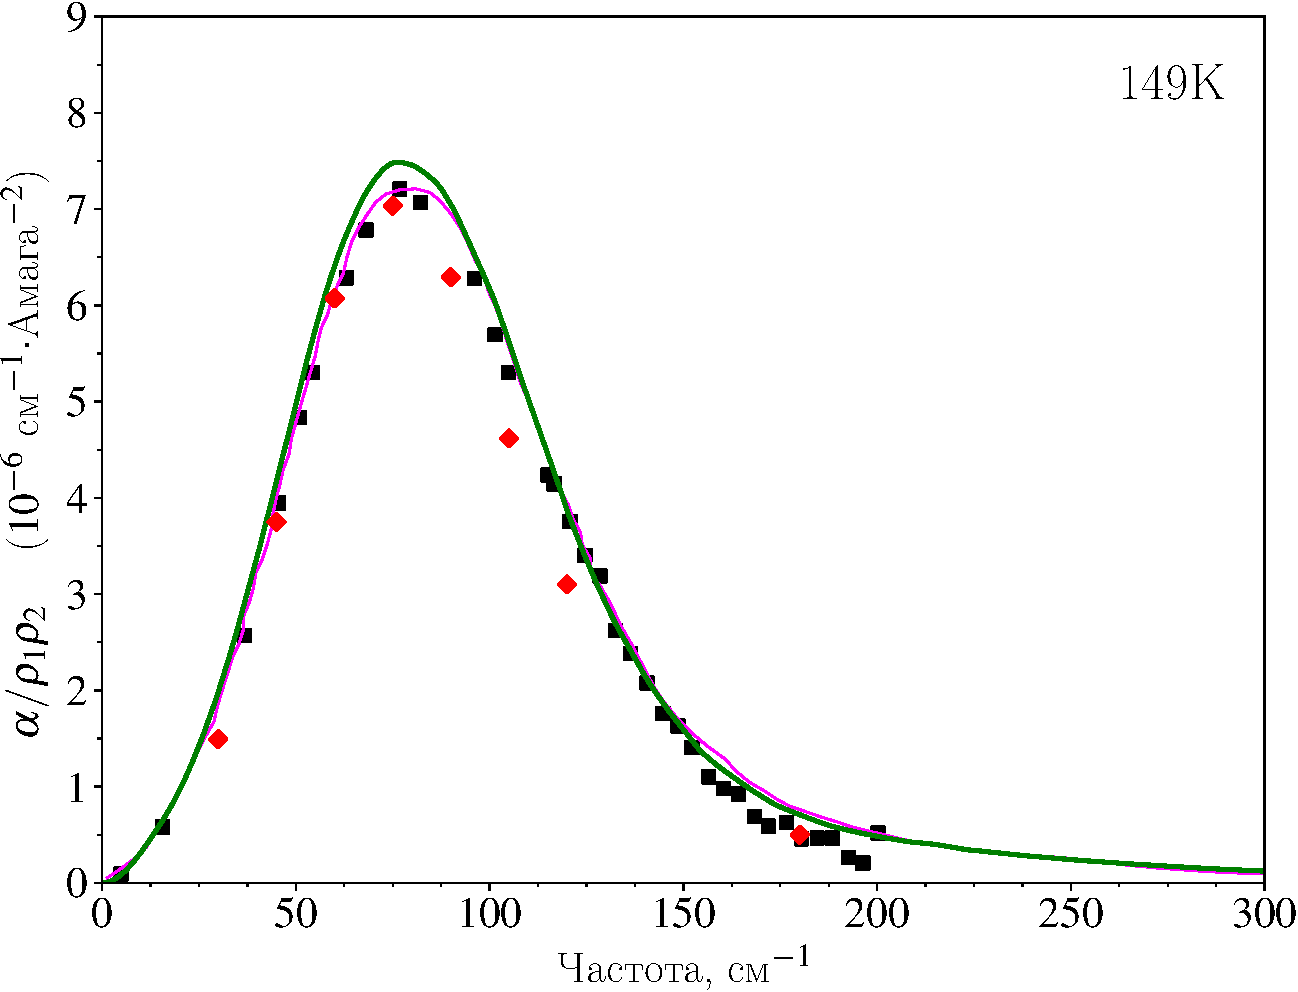
\includegraphics[width=0.49\linewidth]{./pictures/polyatom_spectra/149K_russian-crop.pdf} \\ 
    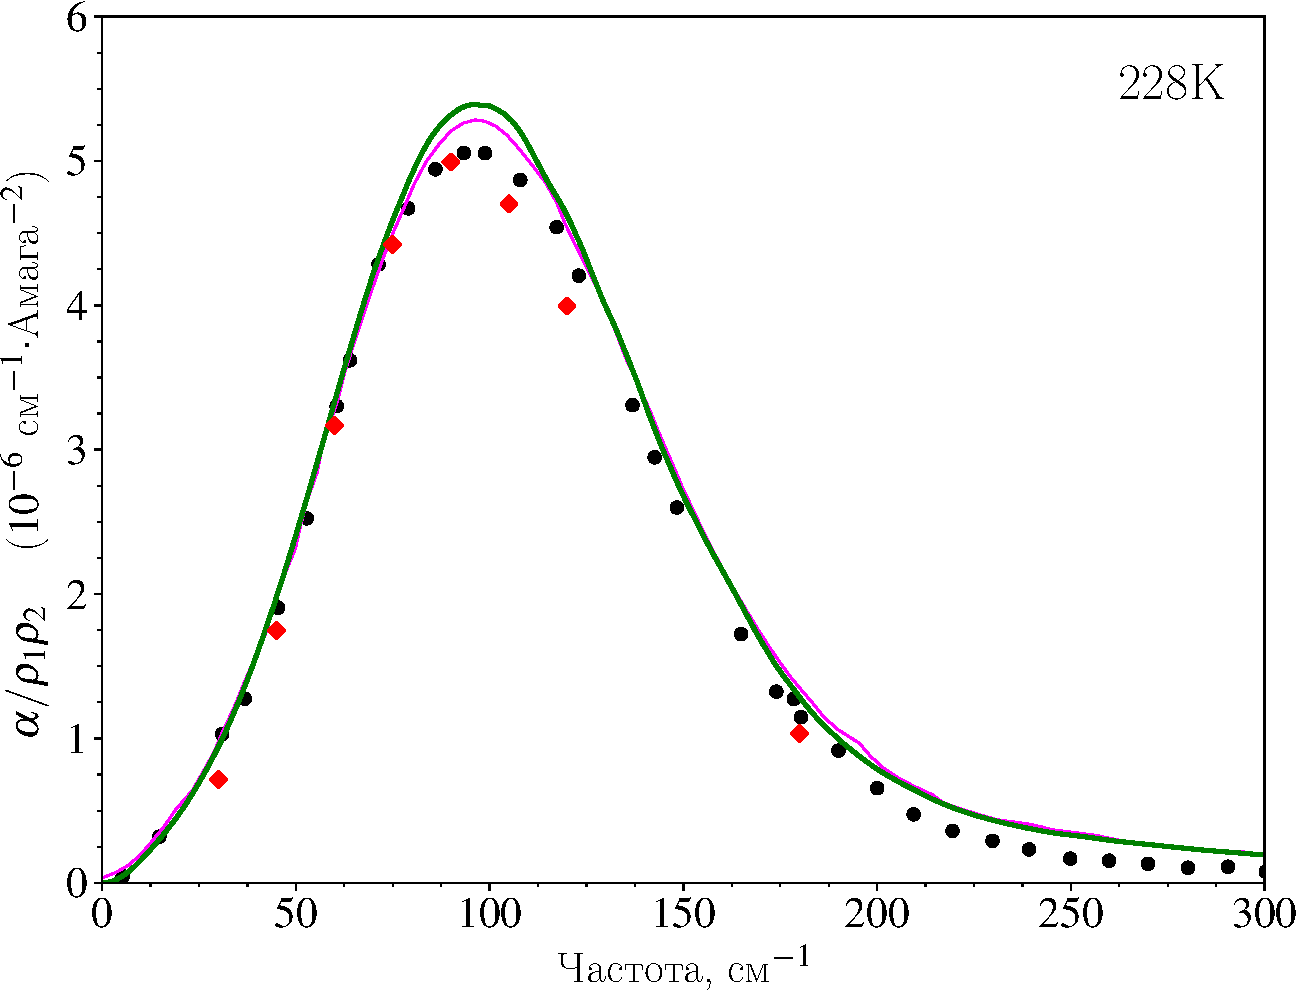
\includegraphics[width=0.49\linewidth]{./pictures/polyatom_spectra/228K_russian-crop.pdf} 
    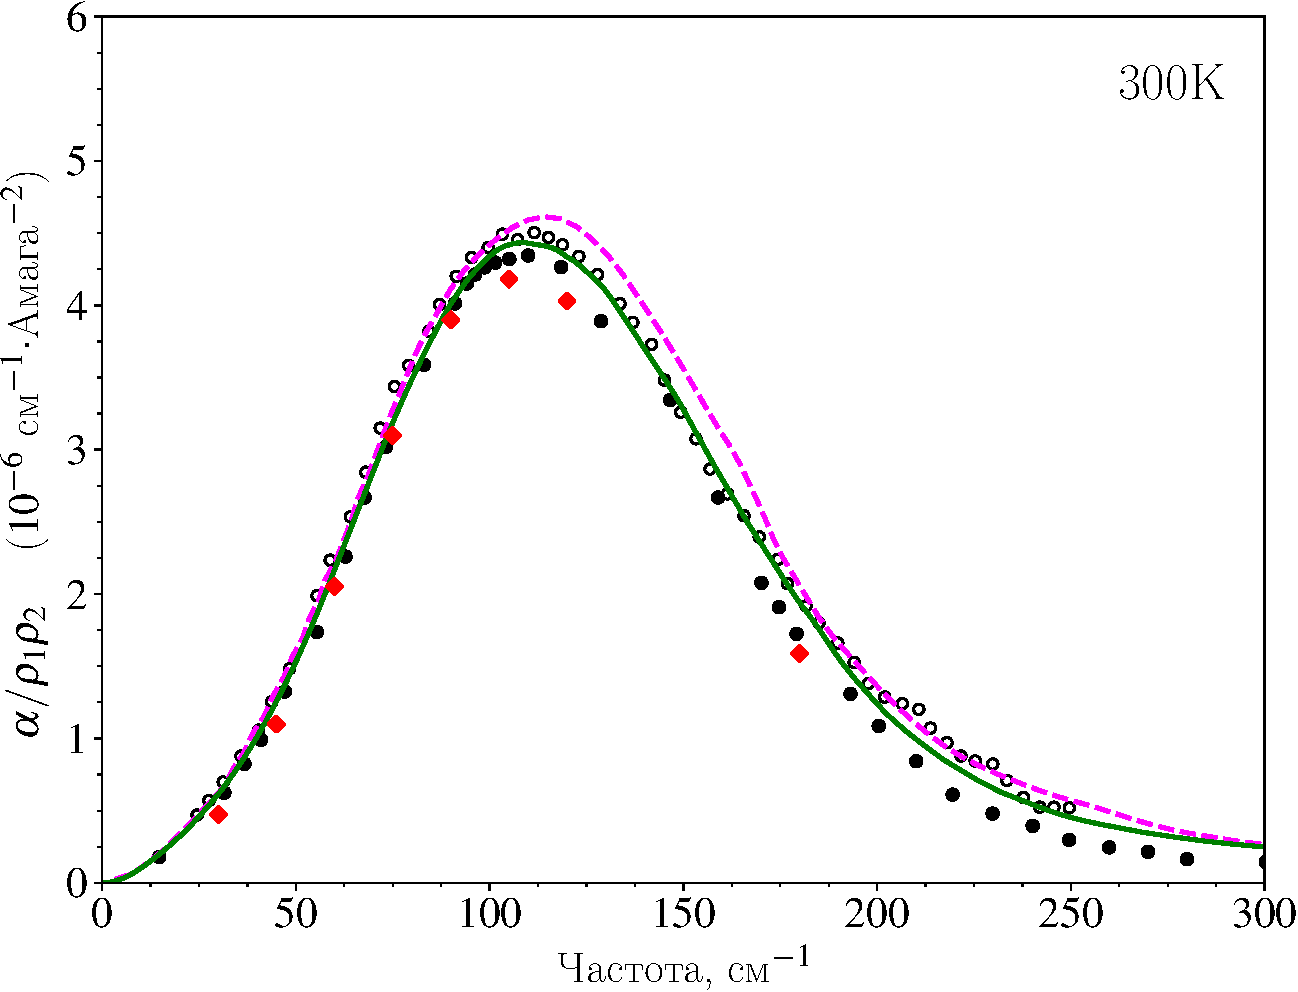
\includegraphics[width=0.49\linewidth]{./pictures/polyatom_spectra/300K_russian-crop.pdf}
    \caption{Сопоставление рассчитанных спектральных профилей системы N$_2-$N$_2$ в области рототрансляционной полосы с расчетными и экспериментальными данными при температурах 89.3K, 109.6K, 129K, 149K, 228K и 300K. Рассчитанные в этой работе профили обозначены жирной зеленой линией. Красными ромбами обозначены интерполированные результаты квантовомеханического расчета \cite{karman2015}. Сиреневой пунктирной линией при температурах 149K, 228K и 300K обозначены результаты молекулярно-динамического расчета \cite{bussery2014}. Тонкой синей линией при температурах 89.3K, 109.6K и 129К обозначены экспериментальные данные из \cite{karman2019}. Коричневой пунктирной линией при температурах 89.3К и 109.6К обозначены результаты изотропного квантово-механического расчета \cite{borysow1986}. Черными кружками при температурах 129K, 228K и 300K обозначены экспериментальные данные из \cite{stone1984}, пустыми кружками при температурах 129К и 300К -- из \cite{buontempo1975}; черными квадратами при температуре 149К -- из \cite{dagg1985}. }  
    \label{fig:n2n2-spectra}
\end{figure}

Траекторные расчеты производились с теми же поверхностями потенциальной энергии и индуцированного дипольного момента, что и квантово-механические расчеты в \cite{karman2015}. Как уже отмечалось при рассмотрении двухатомных спектров, процедура десимметризации D3 переоценивает квантовую спектральную функцию, поэтому расхождения в области крыла спектра могут быть объяснены неточностью десимметризации. Авторы \cite{karman2015} отмечают, что недостаточное количество \textit{ab initio} точек могло вызывать погрешности в коэффициентах сферических функций, используемых для аппроксимации данных. Вклад связанных состояний в интегральную интенсивность при рассматриваемых температурах достаточно невелик
\begin{gather}
    \begin{aligned}
        89.3K  &: \quad M_0^\text{bound} / M_0^\text{full} = 5.5\%, \quad M_2^\text{bound} / M_2^\text{full} = 1.5\%, \\
        109.6K &: \quad M_0^\text{bound} / M_0^\text{full} = 3.0\%, \quad M_2^\text{bound} / M_2^\text{full} = 0.6\%, \\
        129.0K &: \quad M_0^\text{bound} / M_0^\text{full} = 1.8\%, \quad M_2^\text{bound} / M_2^\text{full} = 0.3\%. 
    \end{aligned}
\end{gather}
При более высоких температурах интегральный вклад связанных состояний становится пренебрежимо малым. Тем не менее, несмотря на пренебрежение связанными состояниями в нашем расчете, полученные нами профили по интенсивности более точно согласуются с экспериментальными данными \cite{karman2019}, чем результаты \cite{karman2015} и \cite{borysow1986}. \par
Авторы \cite{karman2019} оценивают погрешность экспериментальных измерений при более низких температурах в 3\% в области максимума спектрального профиля. Для экспериментальных данных \cite{stone1984}, \cite{buontempo1975}, \cite{dagg1985} погрешность оценивается в 10\% в области максимума поглощения. \par
Спектральные профили при низких температурах обладают двумя особенностями на фоне широкого континуального спектра -- в области малых частот наблюдается набор резких пиков и в области максимума спектра наблюдается волнистая структура, часто называемая риплами. Ранее эти особенности были обнаружены для спектра в области фундаментального перехода азота в системах N$_2-$N$_2$ и N$_2-$Ar \cite{mckellar1988}, в рототрансляционной области для системы N$_2-$N$_2$ наблюдались впервые в работе \cite{wishnow1996}. Авторы \cite{mckellar1988}, ссылаясь на теоретический анализ структуры риплов, наблюдаемых в системе N$_2-$Ar \cite{brocks1988}, связывают их с проявлениями связанных и метастабильных состояний. Отметим, что результаты изотропного квантового расчета \cite{borysow1986} обладают волнистой структурой в области максимума. \par 
Контроль сходимости расчета спектров производился при помощи спектральных моментов. Если на всех стадиях расчета не вносятся систематические ошибки, то с увеличением количества траекторий спектральные моменты траекторного спектра должны совпасть со спектральными моментами, посчитанными по области фазового пространства, соответствующей свободным и метастабильным состояниям. Каждый из представленных на рис. (\ref{fig:n2n2-spectra}) получен в результате усреднения по 2.000.000 траекториям. Спектральные моменты посчитаны по области фазового пространства с энергией комплекса больше нуля при помощи адаптивного метода Монте-Карло \cite{hep}. Сравнение спектральных моментов представлено в таблице (\ref{table:n2n2-moments}).

\begin{table}[H]
    \caption{Сравнение спектральных моментов, рассчитанных по фазовому пространству, с моментами по траекторным спектрам системы N$_2-$N$_2$}
    \begin{tabular}{c >{\centering}p{6cm} >{\centering}p{6cm} >{\centering}p{3cm}}
        \toprule
        $T$, K & Спектральные моменты $M_0$ (см$^{-1} \cdot$Амага$^{-2}$) и $M_2$ (см$^{-3} \cdot$Амага$^{-2}$) по фазовому пространству & Спектральные моменты $M_0$ (см$^{-1} \cdot$Амага$^{-2}$) и $M_2$ (см$^{-3} \cdot$Амага$^{-2}$) по траекторному спектру & Отклонение \tabularnewline
        \midrule
        \multirow{2}{*}{$89.3$}  & $5.487\cdot 10^{-5}$ & $5.493 \cdot 10^{-5}$ & $+0.1$ \%  \tabularnewline
                                 & $1.068\cdot 10^{-1}$ & $1.087 \cdot 10^{-1}$ & $+1.7$ \%  \tabularnewline
        \midrule
        \multirow{2}{*}{$109.6$} & $4.817\cdot 10^{-5}$ & $4.826 \cdot 10^{-5}$ & $+0.2$ \%  \tabularnewline
                                 & $1.137\cdot 10^{-1}$ & $1.144 \cdot 10^{-1}$ & $-0.7$ \%  \tabularnewline
        \midrule
        \multirow{2}{*}{$129.0$} & $4.444\cdot 10^{-5}$ & $4.414 \cdot 10^{-5}$ & $+0.7$ \%  \tabularnewline
                                 & $1.227\cdot 10^{-1}$ & $1.232 \cdot 10^{-1}$ & $-0.4$ \%  \tabularnewline
        \midrule
        \multirow{2}{*}{$149.0$} & $4.178\cdot 10^{-5}$ & $4.271 \cdot 10^{-5}$ & $+2.2$ \%  \tabularnewline
                                 & $1.332\cdot 10^{-1}$ & $1.357 \cdot 10^{-1}$ & $+1.9$ \%  \tabularnewline
        \midrule
        \multirow{2}{*}{$228.3$} & $3.756\cdot 10^{-5}$ & $3.768 \cdot 10^{-5}$ & $+0.3$ \%  \tabularnewline
                                 & $1.848\cdot 10^{-1}$ & $1.859 \cdot 10^{-1}$ & $+0.6$ \%  \tabularnewline
        \midrule
        \multirow{2}{*}{$300.0$} & $3.650\cdot 10^{-5}$ & $3.576 \cdot 10^{-5}$ & $-2.0$ \%  \tabularnewline
                                 & $2.389\cdot 10^{-1}$ & $2.339 \cdot 10^{-1}$ & $-2.1$ \%  \tabularnewline
        \bottomrule
    \end{tabular}
    \label{table:n2n2-moments}
\end{table}

На рис. (\ref{fig:co2ar-spectra}) приведено сравнение рассчитанных спектров для системы CO$_2-$Ar с экспериментальными данными из \cite{tonkov1995}. При обеих температурах расхождение в максимуме спектрального профиля с экспериментальными данными составляет около 10-12\%, что попадает в интервал погрешности 10\%, который часто приписывается экспериментальным данным.
Отметим, что при экспериментальном изучении газовой смеси CO$_2-$Ar в изучаемом диапазоне часто поглощают как молекулярные пары CO$_2-$Ar, так и пары CO$_2-$CO$_2$. Максимум поглощения комплекса CO$_2-$CO$_2$ при обеих рассматриваемых температурах находится очень близко к максимуму поглощения комплекса CO$_2-$Ar \cite{gruszka1997}. Следовательно, наблюдаемое расхождение может быть связано и с погрешностями, вызванными определением поглощения комплекса CO$_2-$CO$_2$.

\begin{figure}[H]
    \centering
    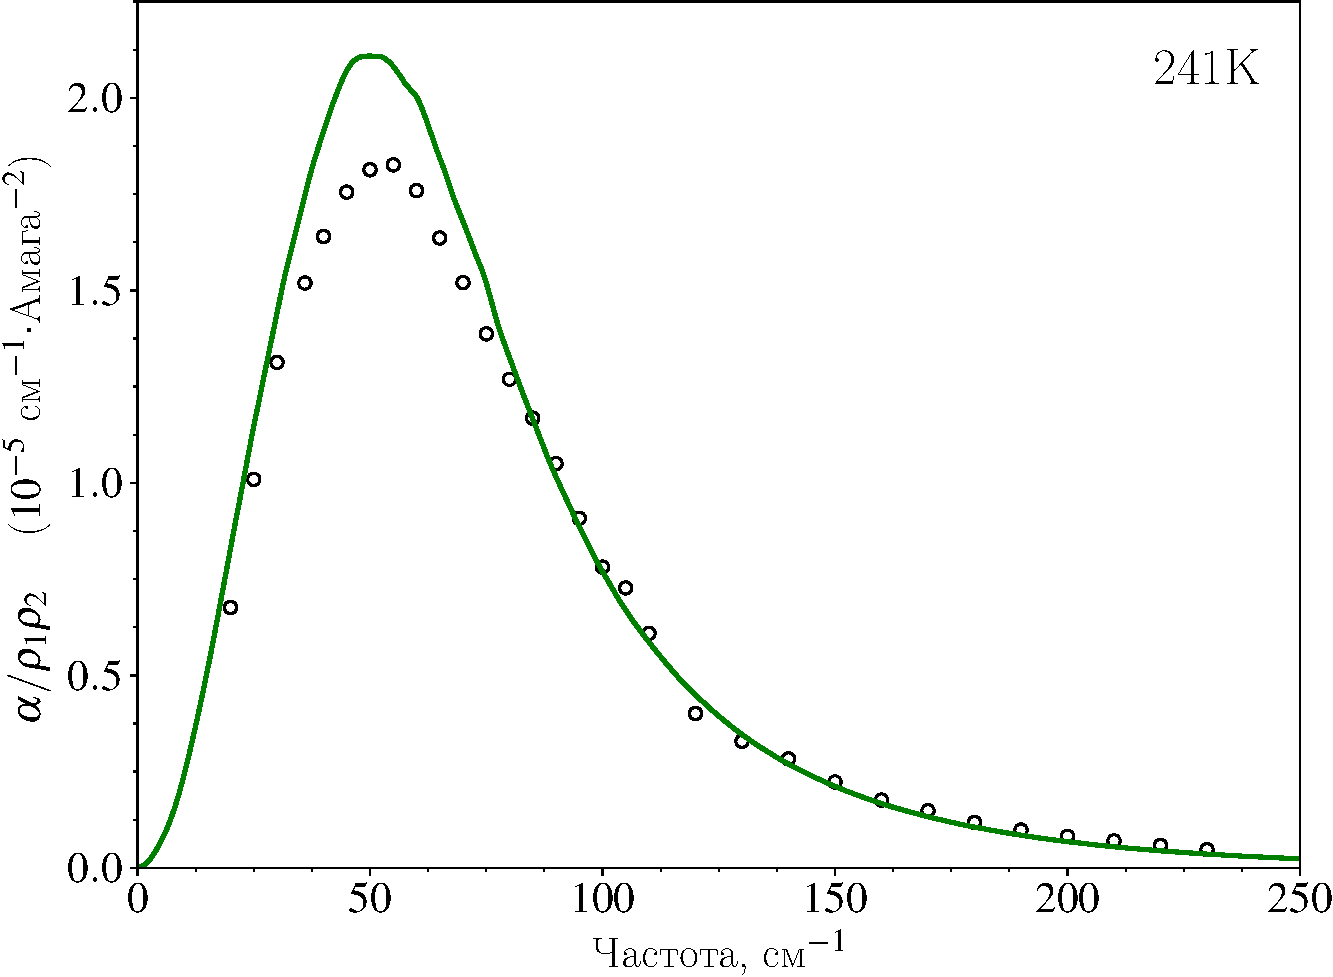
\includegraphics[width=0.49\linewidth]{./pictures/polyatom_spectra/co2_ar/241K_russian-crop.pdf}
    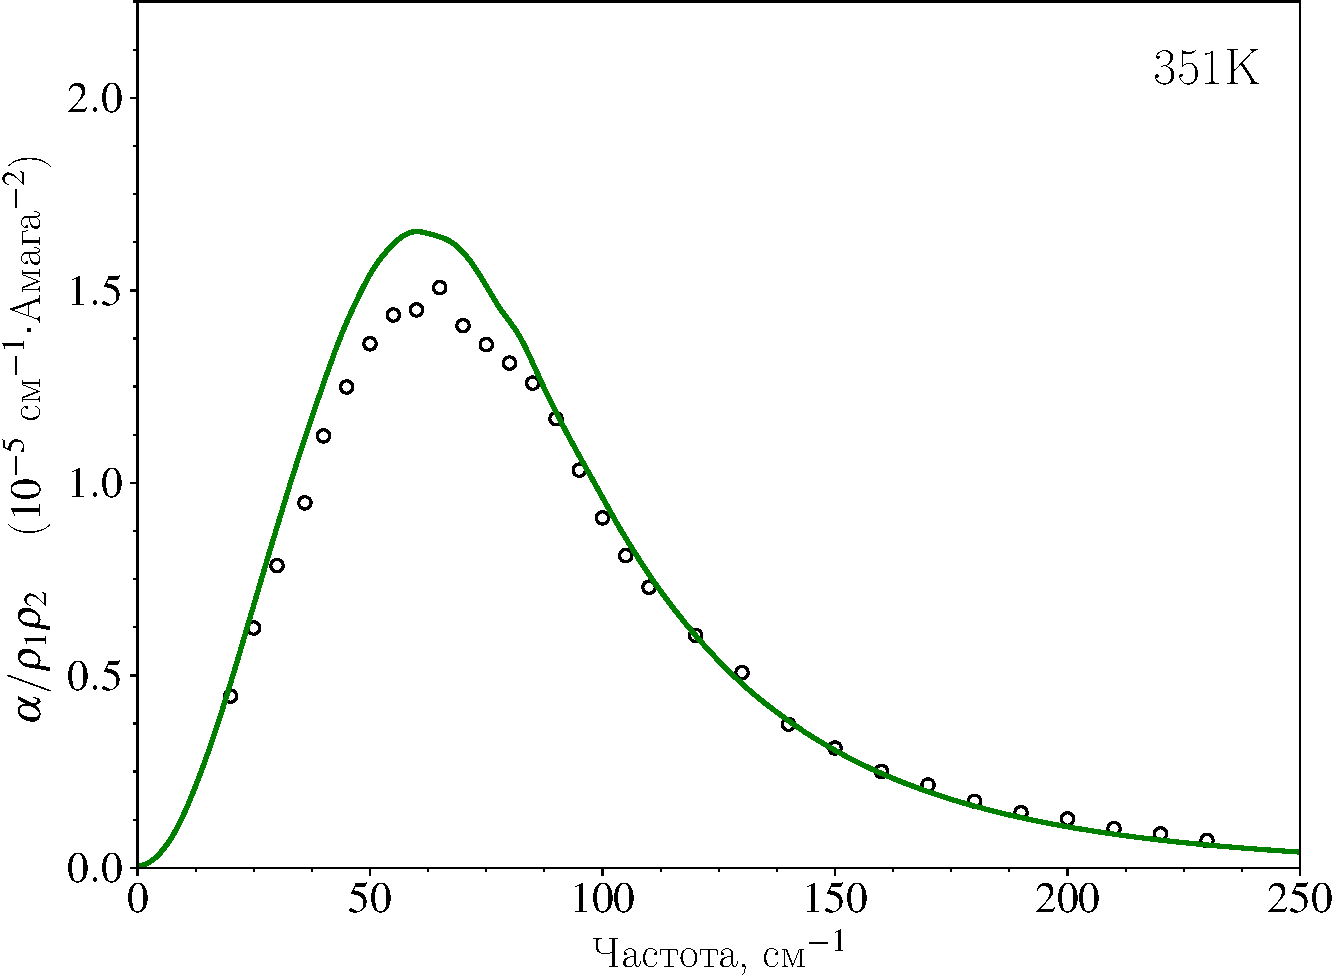
\includegraphics[width=0.49\linewidth]{./pictures/polyatom_spectra/co2_ar/351K_russian-crop.pdf}
    \caption{Сопоставление рассчитанных спектральных профилей системы CO$_2-$Ar в области рототрансляционной полосы с экспериментальными данными из \cite{tonkov1995} при температурах 241K и 351K.}
    \label{fig:co2ar-spectra}
\end{figure}

Каждый из спектров, представленных на рис. (\ref{fig:co2ar-spectra}), получен в результате усреднения по 1.000.000 траекторий. Данные о сходимости расчета по спектральным моментам представлены в таблице (\ref{table:co2ar-moments}). 

\begin{table}[H]
    \caption{Сравнение спектральных моментов, рассчитанных по фазовому пространству, с моментами по траекторным спектрам системы CO$_2-$Ar}
    \begin{tabular}{c >{\centering}p{6cm} >{\centering}p{6cm} >{\centering}p{3cm}}
        \toprule
        $T$, K & Спектральные моменты $M_0$ (см$^{-1} \cdot$Амага$^{-2}$) и $M_2$ (см$^{-3} \cdot$Амага$^{-2}$) по фазовому пространству & Спектральные моменты $M_0$ (см$^{-1} \cdot$Амага$^{-2}$) и $M_2$ (см$^{-3} \cdot$Амага$^{-2}$) по траекторному спектру & Отклонение \tabularnewline
        \midrule
        \multirow{2}{*}{$241.0$} & $3.851 \cdot 10^{-4}$ & $3.730 \cdot 10^{-4}$ & $-3.1$ \%  \tabularnewline
                                 & $5.502 \cdot 10^{-1}$ & $5.417 \cdot 10^{-1}$ & $-1.5$ \%  \tabularnewline
        \midrule
        \multirow{2}{*}{$351.0$} & $3.638 \cdot 10^{-4}$ & $3.493 \cdot 10^{-4}$ & $-0.8$ \%  \tabularnewline
                                 & $7.229 \cdot 10^{-1}$ & $7.276 \cdot 10^{-1}$ & $+0.4$ \%  \tabularnewline
        \bottomrule
    \end{tabular}
    \label{table:co2ar-moments}
\end{table}

\begin{table}[H]
\centering
\caption{Рассчитанные методом классических траекторий значения коэффициентов поглощения, преобразованных при помощи процедуры десимметризации D3, в диапазоне температур от $89.3$K до $300$K для системы N$_2-$N$_2$}
\begin{tabular}{ccccccc}
\toprule
 & \multicolumn{6}{c}{$\alpha(\nu)/\rho_1 \rho_2$, см$^{-1}\cdot$Амага$^{-2}$} \\ 
\cmidrule(lr){2-7} 
$\nu$, см$^{-1}$ & 89.3K & 109.6K & 129.0K & 149.0K & 228.3K & 300.0K \\ 
\midrule
$10$ & \num{7.753e-07} & \num{5.323e-07} & \num{3.896e-07} & \num{3.151e-07} & \num{1.565e-07} & \num{1.010e-07} \\ 
$20$ & \num{2.440e-06} & \num{1.634e-06} & \num{1.181e-06} & \num{9.620e-07} & \num{4.810e-07} & \num{3.203e-07} \\ 
$30$ & \num{5.470e-06} & \num{3.540e-06} & \num{2.505e-06} & \num{1.984e-06} & \num{9.408e-07} & \num{6.149e-07} \\ 
$40$ & \num{9.109e-06} & \num{6.032e-06} & \num{4.333e-06} & \num{3.380e-06} & \num{1.586e-06} & \num{1.011e-06} \\ 
$50$ & \num{1.196e-05} & \num{8.349e-06} & \num{6.268e-06} & \num{4.969e-06} & \num{2.405e-06} & \num{1.529e-06} \\ 
$60$ & \num{1.305e-05} & \num{9.860e-06} & \num{7.779e-06} & \num{6.409e-06} & \num{3.333e-06} & \num{2.166e-06} \\ 
$70$ & \num{1.224e-05} & \num{1.006e-05} & \num{8.484e-06} & \num{7.286e-06} & \num{4.220e-06} & \num{2.848e-06} \\ 
$80$ & \num{1.019e-05} & \num{9.192e-06} & \num{8.237e-06} & \num{7.456e-06} & \num{4.910e-06} & \num{3.490e-06} \\ 
$90$ & \num{7.746e-06} & \num{7.595e-06} & \num{7.270e-06} & \num{7.053e-06} & \num{5.316e-06} & \num{4.009e-06} \\ 
$100$ & \num{5.555e-06} & \num{5.868e-06} & \num{5.990e-06} & \num{6.179e-06} & \num{5.381e-06} & \num{4.339e-06} \\ 
$110$ & \num{3.814e-06} & \num{4.386e-06} & \num{4.723e-06} & \num{5.034e-06} & \num{5.111e-06} & \num{4.430e-06} \\ 
$120$ & \num{2.599e-06} & \num{3.085e-06} & \num{3.480e-06} & \num{3.873e-06} & \num{4.626e-06} & \num{4.336e-06} \\ 
$130$ & \num{1.870e-06} & \num{2.217e-06} & \num{2.494e-06} & \num{2.908e-06} & \num{3.993e-06} & \num{4.101e-06} \\ 
$140$ & \num{1.399e-06} & \num{1.546e-06} & \num{1.789e-06} & \num{2.160e-06} & \num{3.333e-06} & \num{3.702e-06} \\ 
$150$ & \num{1.089e-06} & \num{1.154e-06} & \num{1.321e-06} & \num{1.597e-06} & \num{2.682e-06} & \num{3.283e-06} \\ 
$160$ & \num{8.902e-07} & \num{9.057e-07} & \num{9.882e-07} & \num{1.185e-06} & \num{2.171e-06} & \num{2.803e-06} \\ 
$170$ & \num{7.440e-07} & \num{7.274e-07} & \num{7.729e-07} & \num{9.031e-07} & \num{1.681e-06} & \num{2.357e-06} \\ 
$180$ & \num{6.318e-07} & \num{6.085e-07} & \num{6.350e-07} & \num{7.100e-07} & \num{1.289e-06} & \num{1.944e-06} \\ 
$190$ & \num{5.357e-07} & \num{5.181e-07} & \num{5.269e-07} & \num{5.720e-07} & \num{9.984e-07} & \num{1.562e-06} \\ 
$200$ & \num{4.560e-07} & \num{4.425e-07} & \num{4.501e-07} & \num{4.833e-07} & \num{7.904e-07} & \num{1.243e-06} \\ 
$210$ & \num{3.859e-07} & \num{3.847e-07} & \num{3.880e-07} & \num{4.217e-07} & \num{6.383e-07} & \num{9.985e-07} \\ 
$220$ & \num{3.253e-07} & \num{3.318e-07} & \num{3.368e-07} & \num{3.662e-07} & \num{5.165e-07} & \num{8.072e-07} \\ 
$230$ & \num{2.720e-07} & \num{2.836e-07} & \num{2.954e-07} & \num{3.175e-07} & \num{4.338e-07} & \num{6.549e-07} \\ 
$240$ & \num{2.294e-07} & \num{2.423e-07} & \num{2.541e-07} & \num{2.757e-07} & \num{3.727e-07} & \num{5.443e-07} \\ 
$250$ & \num{1.924e-07} & \num{2.074e-07} & \num{2.207e-07} & \num{2.410e-07} & \num{3.324e-07} & \num{4.538e-07} \\ 
$260$ & \num{1.625e-07} & \num{1.777e-07} & \num{1.903e-07} & \num{2.111e-07} & \num{2.940e-07} & \num{3.938e-07} \\ 
$270$ & \num{1.351e-07} & \num{1.494e-07} & \num{1.631e-07} & \num{1.854e-07} & \num{2.642e-07} & \num{3.445e-07} \\ 
$280$ & \num{1.137e-07} & \num{1.256e-07} & \num{1.410e-07} & \num{1.628e-07} & \num{2.369e-07} & \num{3.052e-07} \\ 
$290$ & \num{9.465e-08} & \num{1.071e-07} & \num{1.217e-07} & \num{1.408e-07} & \num{2.136e-07} & \num{2.734e-07} \\ 
$300$ & \num{7.946e-08} & \num{9.042e-08} & \num{1.042e-07} & \num{1.221e-07} & \num{1.928e-07} & \num{2.485e-07} \\ 
$310$ & \num{6.635e-08} & \num{7.680e-08} & \num{8.895e-08} & \num{1.061e-07} & \num{1.747e-07} & \num{2.259e-07} \\ 
$320$ & \num{5.614e-08} & \num{6.502e-08} & \num{7.667e-08} & \num{9.194e-08} & \num{1.595e-07} & \num{2.080e-07} \\ 
$330$ & \num{4.733e-08} & \num{5.472e-08} & \num{6.533e-08} & \num{7.993e-08} & \num{1.427e-07} & \num{1.917e-07} \\ 
$340$ & \num{4.004e-08} & \num{4.623e-08} & \num{5.619e-08} & \num{6.853e-08} & \num{1.278e-07} & \num{1.768e-07} \\ 
$350$ & \num{3.388e-08} & \num{3.923e-08} & \num{4.822e-08} & \num{5.916e-08} & \num{1.142e-07} & \num{1.618e-07} \\ 
$360$ & \num{2.873e-08} & \num{3.324e-08} & \num{4.138e-08} & \num{5.098e-08} & \num{1.018e-07} & \num{1.476e-07} \\ 
$370$ & \num{2.441e-08} & \num{2.830e-08} & \num{3.523e-08} & \num{4.403e-08} & \num{9.049e-08} & \num{1.352e-07} \\ 
$380$ & \num{2.076e-08} & \num{2.409e-08} & \num{3.018e-08} & \num{3.823e-08} & \num{8.049e-08} & \num{1.221e-07} \\ 
$390$ & \num{1.771e-08} & \num{2.059e-08} & \num{2.599e-08} & \num{3.315e-08} & \num{7.174e-08} & \num{1.113e-07} \\ 
$400$ & \num{1.514e-08} & \num{1.762e-08} & \num{2.229e-08} & \num{2.872e-08} & \num{6.375e-08} & \num{1.006e-07} \\ 
\bottomrule 
\end{tabular}
\label{table:n2n2-spectra}
\end{table}

%\begin{subappendices}
    \chapter*{Приложение 4.А}
    %\section{Вектор углового момента в подвижной системе отсчета} \label{appendix:angular-momentum-body-fixed}
    {\Large\textbf{Вектор углового момента в подвижной системе отсчета}} \label{appendix:angular-momentum-body-fixed}
    \vspace{0.5cm}
    \addcontentsline{toc}{chapter}{Приложение 4.A. Вектор углового момента в подвижной системе отсчета}
    
    Рассмотрим производную кинетической энергии в лагранжевой форме $\Tl$ по вектору угловой скорости $\bOmega$, компоненты которого выражены в подвижной системе отсчета. Продифференцировав выражение \eqref{body-fixed-lagrange-energy} по вектору угловой скорости, получаем 
    \begin{gather}
        \frac{\partial \Tl}{\partial \bOmega} = \bbA \dot{\mf{q}} + \bbI \bOmega. \label{appendix-angular-momentum1}
    \end{gather}

    Несложно показать, что вектор углового момента $\mf{j}$ в лабораторной системе отсчета может быть записан через векторы Якоби как
    \begin{gather}
        \mf{j} = \sum_{i = 1}^{N - 1} \mu_i \lsq \bs{\rho}_i \times \dot{\bs{\rho}}_i \rsq. \label{appendix-angular-momentum-jacobi-vectors}
    \end{gather}

    Выразим производную вектора $\bs{\rho}_i$ в лабораторной системе координат через производную в подвижной системе координат 
    \begin{gather}
        \dot{\bs{\rho}}_i = \bbS^{-1} \lb \dot{\mf{R}}_i + \lsq \bs{\Omega} \times \mf{R}_i \rsq \rb. \label{appendix-jacobi-vector-derivative} 
    \end{gather}

    Подставив выражение \eqref{appendix-jacobi-vector-derivative} в выражение углового момента \eqref{appendix-angular-momentum-jacobi-vectors} и осуществив несложные алгебраические преобразования, приходим к 
    \begin{gather}
        \mf{j} = \sum_{i = 1}^{N-1} \mu_i \lsq \bs{\rho}_i \times \bbS^{-1} \lb \dot{\mf{R}}_i + \Big[ \bOmega \times \mf{R}_i \Big] \rb \rsq = \bbS^{-1} \sum_{i = 1}^{N-1} \mu_i \Big[ \mf{R}_i \times \dot{\mf{R}}_i \Big] + \bbS^{-1} \sum_{i = 1}^{N-1} \mu_i \Big[ \mf{R}_i \times \lsq \bOmega \times \mf{R}_i \rsq \Big] = \bbS^{-1} \lb \bbA \dot{\mf{q}} + \bbI \bOmega \rb.
    \end{gather}

    Умножая обе части на матрицу $\bbS$, получаем в правой части выражение \eqref{appendix-angular-momentum1}
    \begin{gather}
        \bbS \mf{j} = \bbA \dot{\mf{q}} + \bbI \bOmega.
    \end{gather}

    Согласно введенному определению матрицы $\bbS$, выражение в левой части есть вектор углового момента в подвижной системе отсчета. Таким образом, мы показали, что производная кинетической энергии в лагранжевой форме по вектору угловой скорости в подвижной системе равна вектору углового момента в подвижной системе
    \begin{gather}
        \mf{J} = \frac{\partial \Tl}{\partial \bOmega}.
    \end{gather}
    
%\end{subappendices}

%\section{Существующие методы моделирования столкновительно-индуцированных спектров}
%\section{Координаты Якоби}
%\section{Гамильтониан в подвижной системе отсчета}
%\section{Сравнение динамических систем уравнений}
%\section{Классический подход в подвижной системе координат}
%\section{Генерация начальных условий}
%\section{Сравнение с экспериментальными данными}

\chapter{Выводы}

% можно попытаться докрутить свой bst-file, пока лень
%\bibliographystyle{mybst}
\bibliographystyle{unsrt}

\bibliography{biblio}

\end{document}
